\documentclass[11pt,a4paper]{article}

% ------------------------------------------------------------------
% Packages
% ------------------------------------------------------------------
\usepackage[utf8]{inputenc}
\usepackage[T1]{fontenc}
\usepackage{lmodern}
\usepackage[margin=2.5cm]{geometry}
\usepackage{amsmath,amssymb}
\usepackage{graphicx}
\usepackage{booktabs}
\usepackage{tabularx}
\usepackage{float}
\usepackage[font=small,labelfont=bf]{caption}
\usepackage{subcaption}
\usepackage{xcolor}
\usepackage[hidelinks]{hyperref}

% Figures are expected in a folder named figures/ next to this file
\graphicspath{{figures/}}
\emergencystretch=2em

% Marker for statements that still need a source or a check
\newcommand{\checkme}[1]{\textcolor{red}{[#1]}}

\title{\textbf{Media Coverage and Online Search Interest\\ during French Health Awareness Campaigns:\\
Granger Causality and Transfer Functions\\ beyond the Campaign Calendar}}
\author{Timothee Roina\\[4pt]
\small Supervised by Marie-Laure Charpignon}
\date{}

\begin{document}
\maketitle

\begin{abstract}
Whether media coverage and public interest follow each other during health awareness campaigns is rarely quantified. We study four recurring French campaigns (Octobre Rose, Movember, Mars Bleu, Dry January) over eleven seasons (2015--2025), combining Google Trends (GT), which measures what people search for online, with MediaCloud (MC) counts of press articles. Coverage and searches peak together for Octobre Rose and Dry January, while for Movember coverage peaks a median of nine days after searches. Because the campaign calendar and the weekly cycle drive both series, we compare linear and nonlinear (kernel) Granger tests with the same tests run on data in which one series comes from another season, and we estimate transfer functions on series stripped of the calendar. Simulations with a known truth show that the shared calendar alone produces the links that standard tests report in seven of eight campaign--direction pairs. One nonlinear link stands out: for Movember, media coverage predicts later searches (Holm-adjusted $p=0.008$), after removing the weekly cycle and the differences between seasons. Beyond the calendar, searches and coverage move together on the same day during Movember, Mars Bleu and Dry January. These associations are predictive, not evidence of a causal effect.
\end{abstract}

\noindent\textbf{Keywords:} infodemiology; digital health; health awareness campaigns; Google Trends; media coverage; Granger causality.

% ==================================================================
\section{Introduction}
% ==================================================================
Recurring awareness campaigns such as Octobre Rose (breast cancer), Movember (prostate cancer), Mars Bleu (colorectal cancer) and Dry January (alcohol) are now firmly embedded in the French public health calendar. Substantial public resources are devoted to prevention, yet the population-level effectiveness of these campaigns remains difficult to evaluate. Digital traces offer a scalable, low-cost complement to traditional surveys: infodemiology, the study of the distribution and determinants of health information in electronic media \cite{eysenbach2009}, has established online search data, and Google Trends in particular, as a measure of public interest in health topics \cite{nuti2014}.

\paragraph{Related work.} Search data have been used to evaluate awareness campaigns one channel at a time. Breast Cancer Awareness Month raises breast-cancer searches every October \cite{glynn2011}; Spanish-language prostate-cancer searches rise during Movember, less than breast-cancer searches do in October \cite{gonzalezpadilla2021}; and for the Great American Smokeout, news coverage, searches and quitline calls all rise on the day of the event \cite{ayers2016}. These studies compare a campaign period with a baseline; they do not ask how the media and the public respond to \emph{each other} during a campaign. That question belongs to agenda-setting research, where the prominence of a topic in the media is expected to shape how important the public finds it \cite{mccombs1972}. Studies pairing news volume with search volume report both directions: news coverage of a political rumour predicted subsequent searches about it \cite{weeks2010}, whereas across 193 countries search interest Granger-caused news attention about twice as often as the reverse \cite{kwak2018}. Granger causality \cite{granger1969} is the standard tool in this literature.

\paragraph{The problem.} Campaign data violate a central assumption of Granger causality: that no unobserved variable drives both series. Two calendars do. The campaign calendar raises press coverage and searches on the same dates every year, and the weekly cycle lowers both at weekends. Either can make one series ``predict'' the other without any day-to-day link between them.

\paragraph{Question and contributions.} We ask: \emph{during health awareness campaigns, does media coverage help predict public search interest, or the reverse, beyond the calendars that drive both; and if so, how large is the response, after what delay, and for how long?} We study the relationship between press coverage, measured with MediaCloud, and online search interest, measured with Google Trends, the first link of the cascade from awareness to information-seeking, screening and care. Our contributions are: (i) a linear and nonlinear (kernel) Granger analysis with lags restricted to each campaign season; (ii) season-swap surrogate tests, which remove the contribution of a fixed campaign calendar, repeated after removing the weekly cycle, the level of each season and the campaign profile in turn, to see what each link depends on; (iii) transfer functions estimated on calendar-adjusted series, which express the links as a delay, a gain and a persistence, separating same-day association from lagged response; and (iv) a check of every procedure on simulated seasonal systems in which the true answer is known.

% ==================================================================
\section{Data}\label{sec:data}
% ==================================================================
\paragraph{Google Trends (GT).} GT provides a relative search volume (RSV) index (0--100) of Google searches in a given geographic area, where 100 corresponds to the maximum over the requested period. Data were retrieved for France with \texttt{PyTrends}. The temporal granularity depends on the requested range: daily below nine months, weekly between nine months and five years, and monthly beyond five years. Monthly series span 2015--2025; campaign windows (Section~\ref{sec:windows}) are retrieved at daily resolution, one request per season, so that 100 corresponds to the busiest day of each season.

\paragraph{MediaCloud (MC).} MC is an open-source platform indexing online news \cite{roberts2021}. We query a collection of French national news outlets through the MediaCloud API using keyword queries, extract article URLs and full texts with \texttt{newspaper3k}, and derive a media-exposure indicator from daily article counts, divided by their seasonal maximum and multiplied by 100.

\paragraph{Query construction.} Lay search vocabulary and editorial vocabulary differ, so queries were optimised separately for each channel (Appendix~\ref{app:queries}). For GT, we used iterative snowball sampling: starting from the campaign name, related terms were added over successive rounds and then curated manually; the signal converges to a stable shape after a few rounds (Figure~\ref{fig:snowball}). For MC, we extracted the most frequent bigrams and trigrams (k-grams) from an initial corpus of articles (Figure~\ref{fig:kgrams}) and retained the relevant ones after manual curation. Figure~\ref{fig:overview} shows the resulting monthly series.

\paragraph{Data quality.} Optimised queries address the relevance of what is counted, but three properties of the sources remain. First, Google Trends values are computed from a sample of searches whose composition is not disclosed, so they ``may slightly vary depending on the time of retrieval'', and a value of 0 does not necessarily mean that there were no searches \cite{mavragani2019}; each seasonal window was retrieved once, and repeating and averaging downloads would reduce this noise. Second, both series are normalised within each season (to the busiest day for GT, to the maximum daily article count for MC), so levels are not comparable across seasons; the analyses therefore rely on within-season dynamics, and seasons are compared only after this normalisation. Third, MediaCloud covers French national online news outlets only, not regional press, television or social media, and the size of the collection changes over time; daily counts are not divided by the total volume of the collection, and normalising within each season absorbs slow changes in collection size but not changes within a season. Finally, the MediaCloud files do not record the exact query that produced them (Appendix~\ref{app:queries}).

\paragraph{Reproducibility.} Code, daily data and all result tables are available at \url{https://github.com/timothee-roi/publichealth-campaigns-datascience}.

\begin{figure}[htbp]
  \centering
  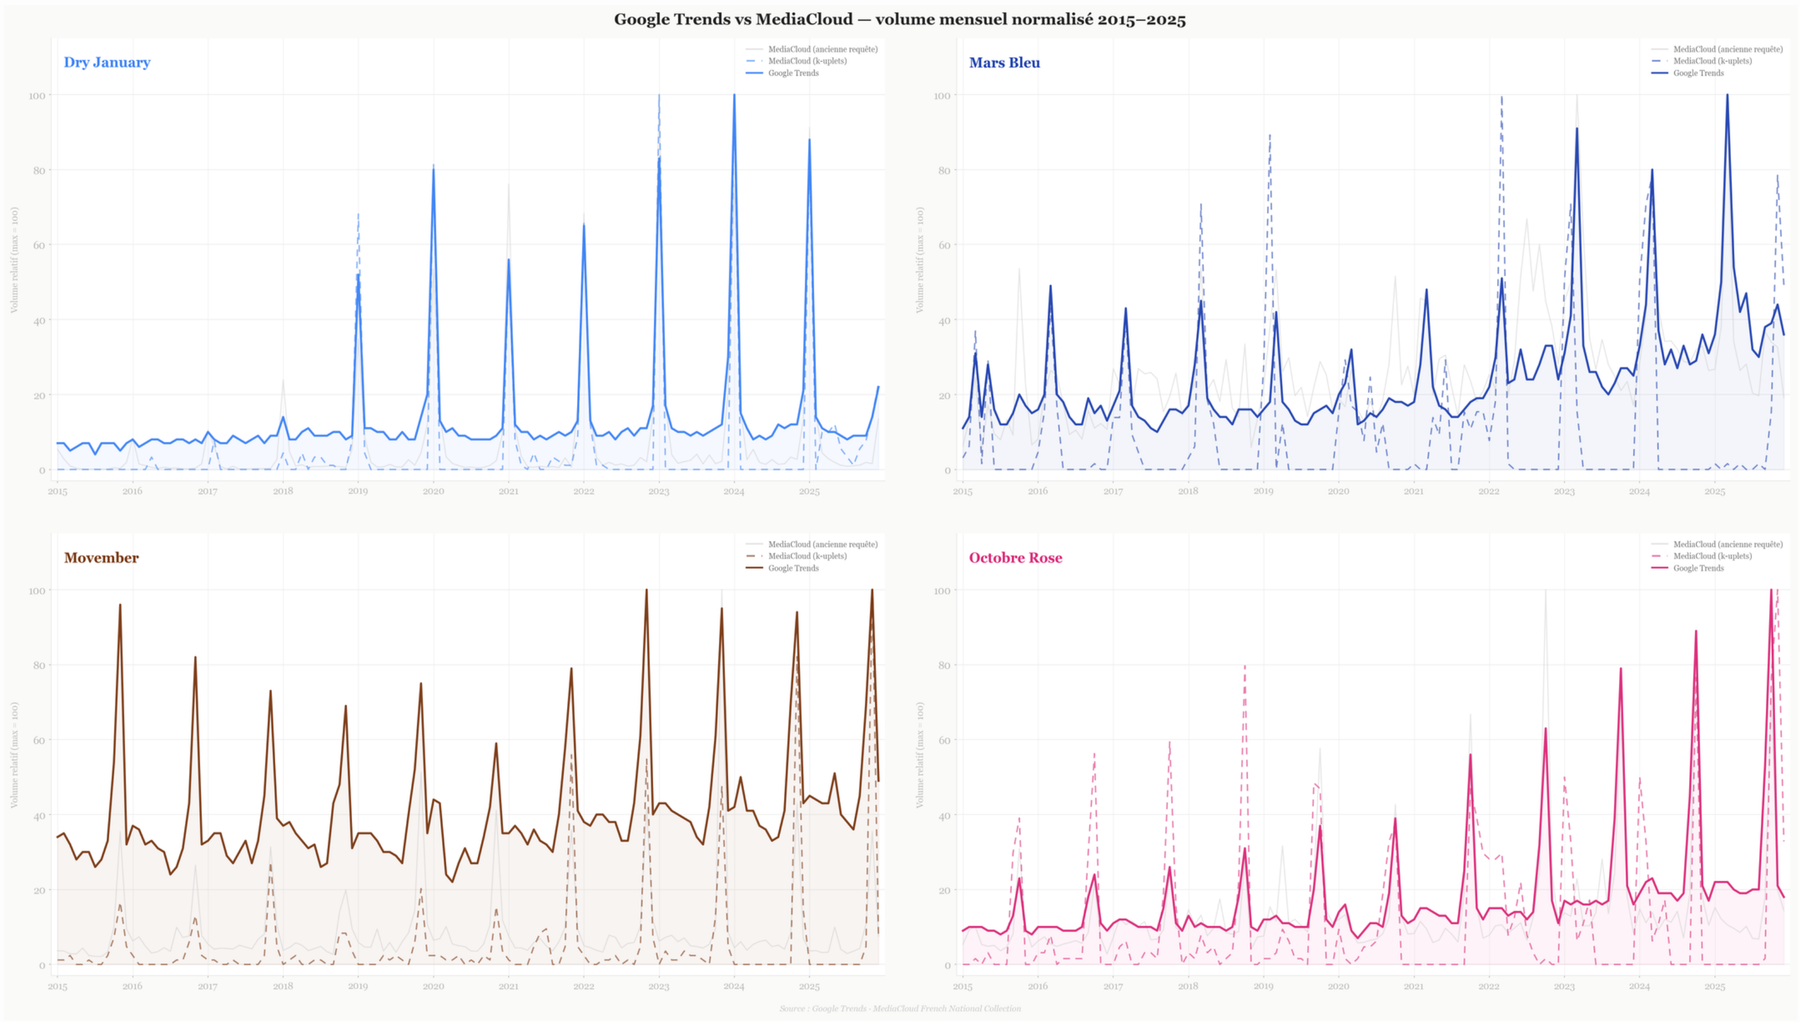
\includegraphics[width=\linewidth]{figure2}
  \caption{Monthly Google Trends and MediaCloud series for the four campaigns, 2015--2025, with optimised queries (each series normalised to a maximum of 100).}
  \label{fig:overview}
\end{figure}

% ==================================================================
\section{Methods}
% ==================================================================
\subsection{Seasonal windows}\label{sec:windows}
Because each campaign is concentrated in a few weeks per year, the analysis is restricted to daily data within a window around each annual campaign: Octobre Rose from 1 September to 30 November (91 days), Movember from 1 October to 31 December (92 days), Mars Bleu from 2 February to 30 April (88--89 days), and Dry January from 26 December to 6 February (43 days), for 11 seasons per campaign. Each season is then aligned on its GT peak (Figures~\ref{fig:peaks1}--\ref{fig:peaks2}), which directly reveals the lead--lag structure between the media peak and the search peak. Figure~\ref{fig:daily} shows the daily series of all seasons.

\begin{figure}[htbp]
  \centering
  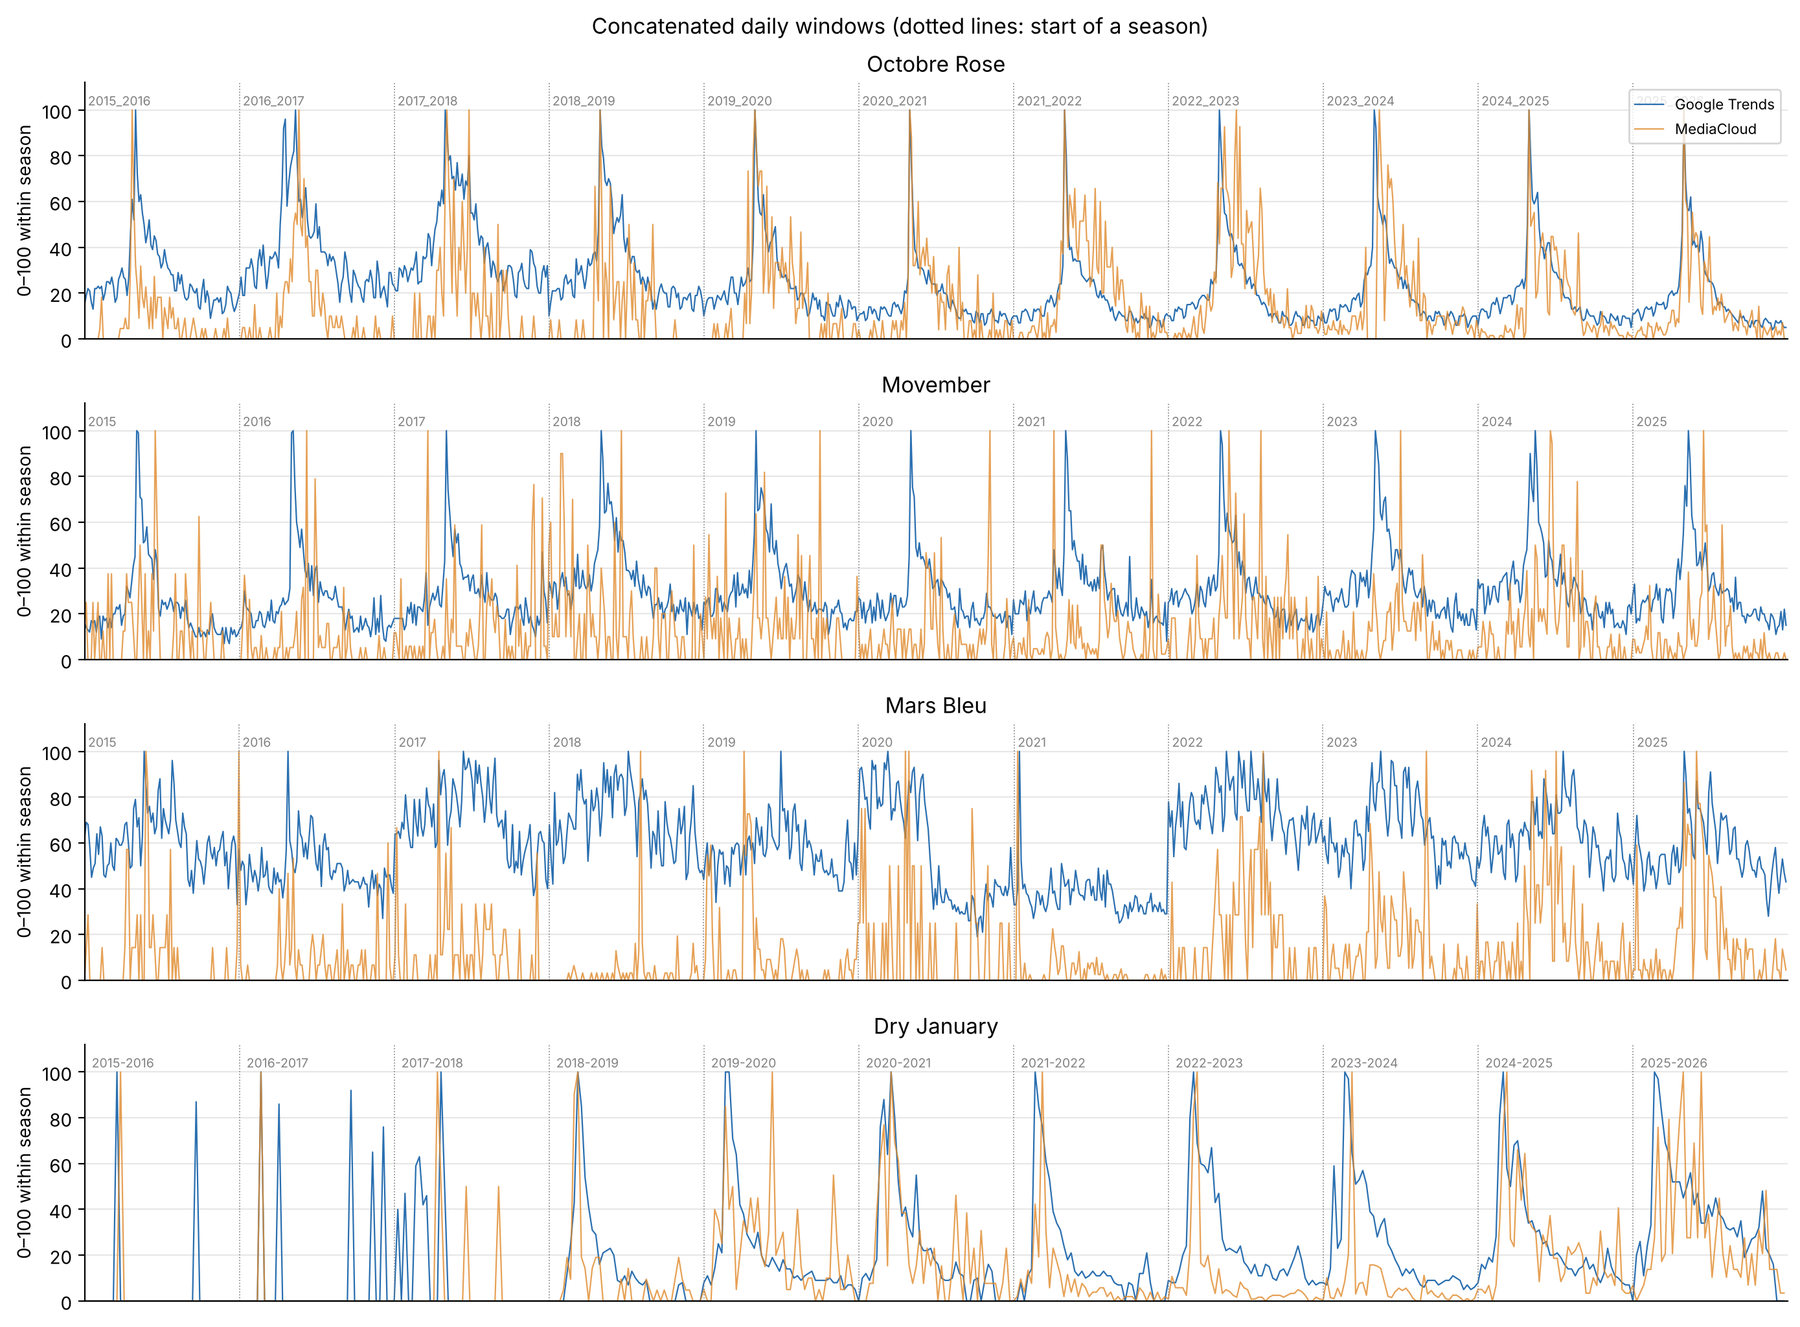
\includegraphics[width=\linewidth]{daily_windows_overview}
  \caption{Daily GT and MC series in the campaign windows, all seasons placed one after the other (each series normalised to 0--100 within each season; dotted lines: start of a season).}
  \label{fig:daily}
\end{figure}

\begin{figure}[htbp]
  \centering
  \begin{subfigure}[t]{0.49\linewidth}
    \centering
    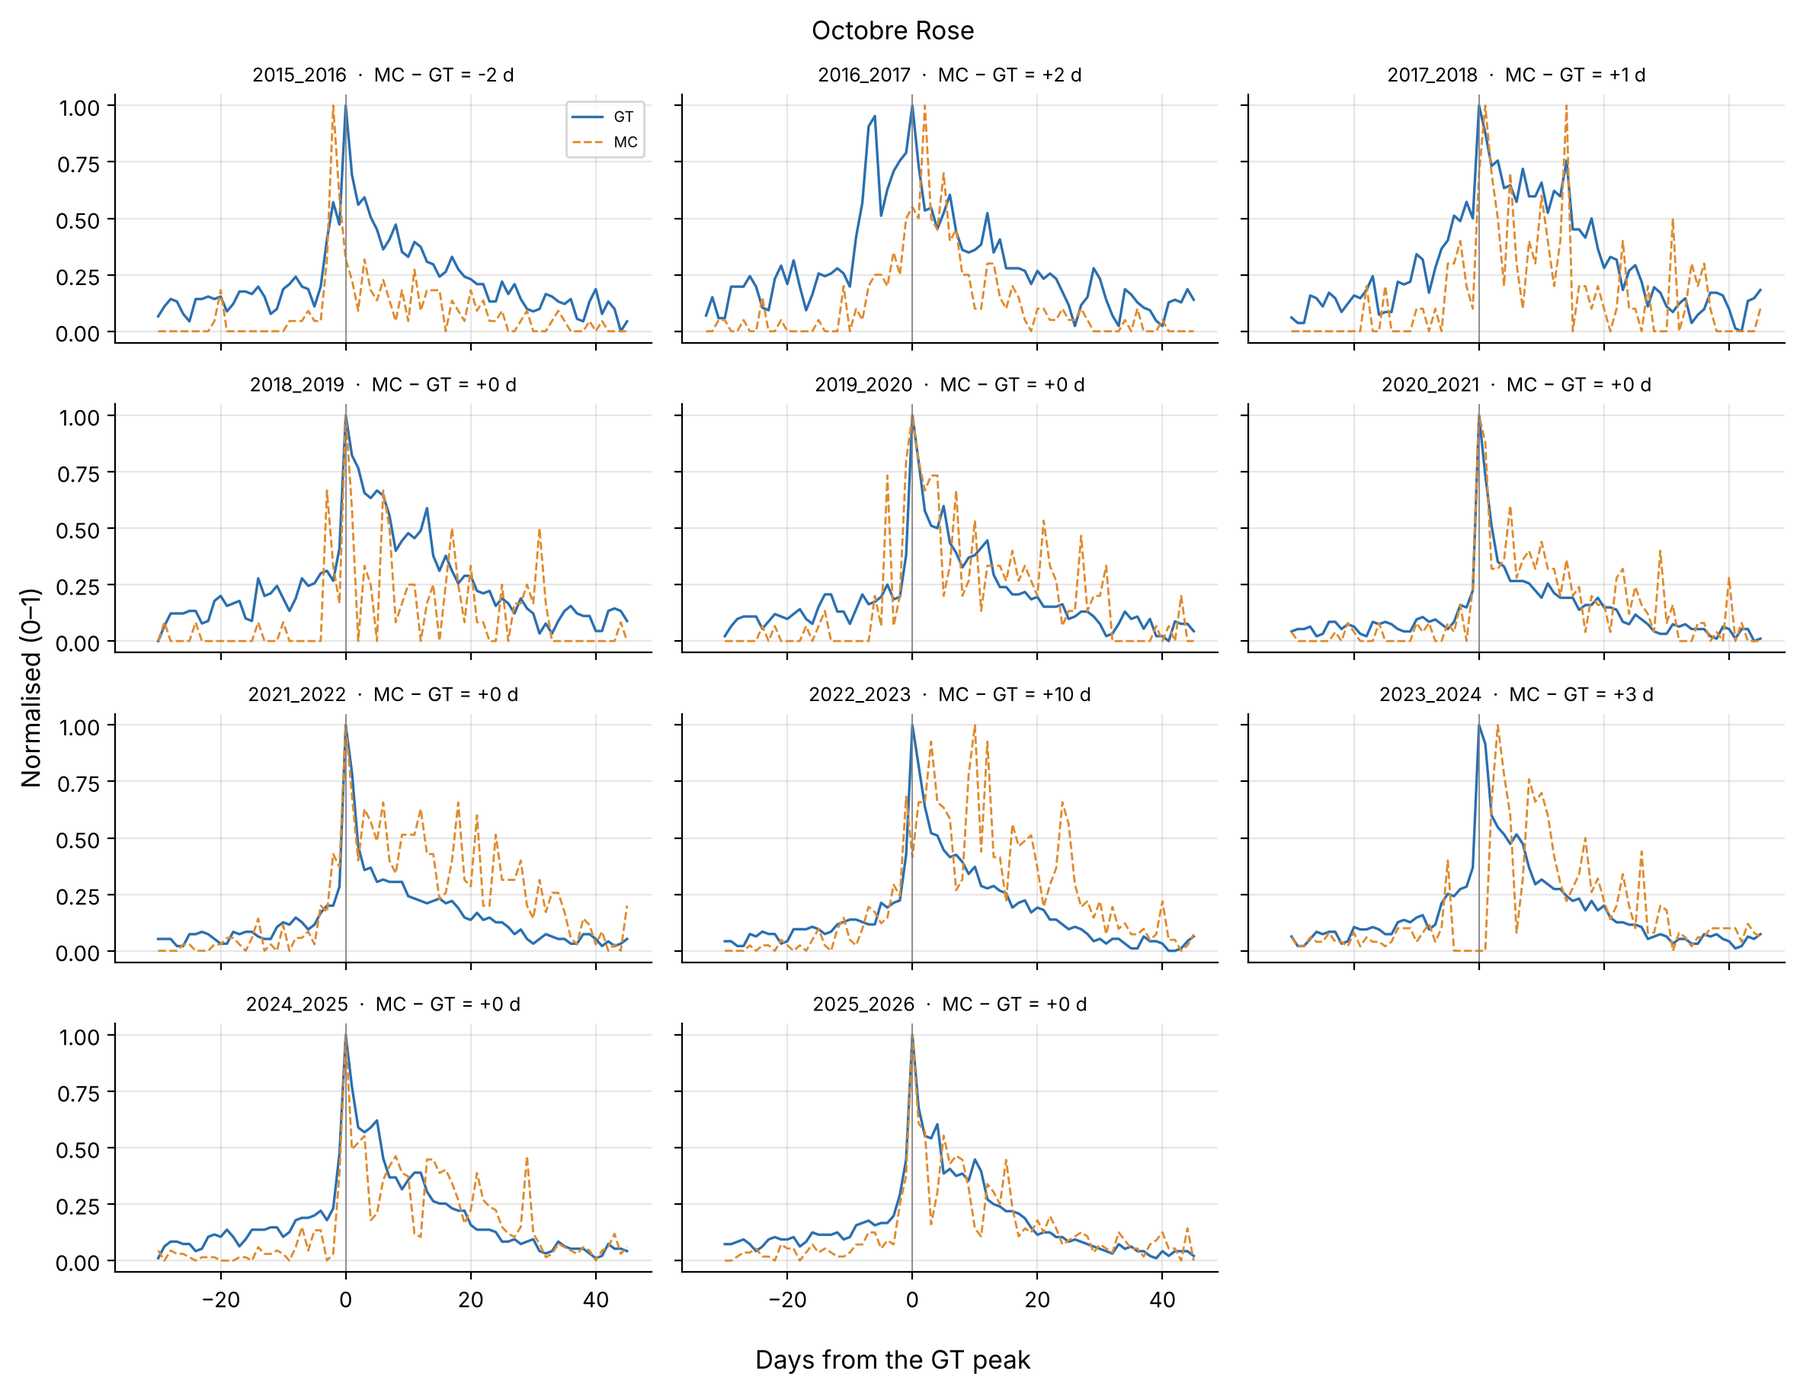
\includegraphics[width=\linewidth]{figure3-1}
    \caption{Octobre Rose}
    \label{fig:peaks1-or}
  \end{subfigure}\hfill
  \begin{subfigure}[t]{0.49\linewidth}
    \centering
    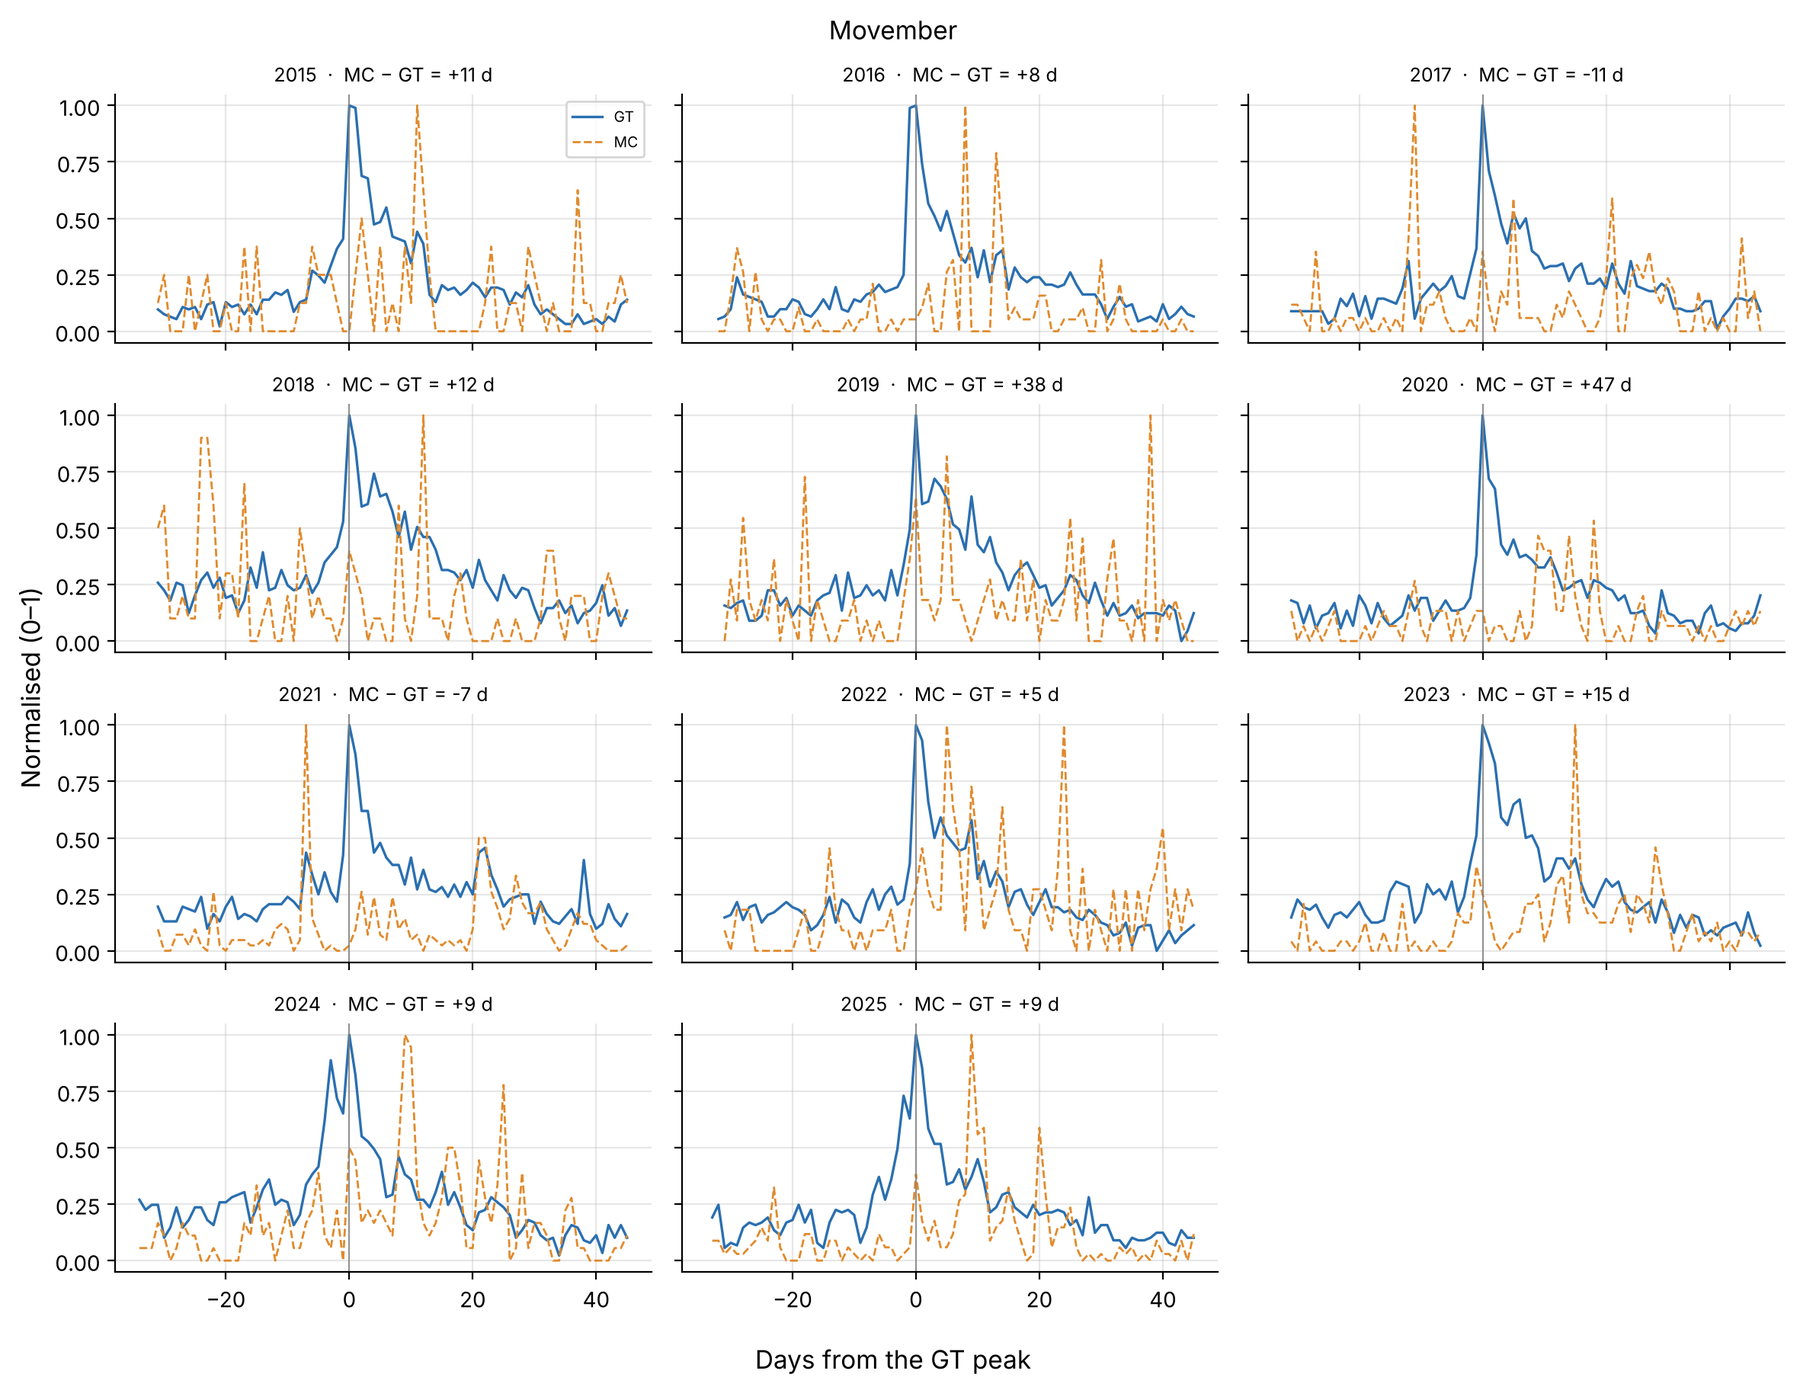
\includegraphics[width=\linewidth]{figure3-2}
    \caption{Movember}
    \label{fig:peaks1-mo}
  \end{subfigure}
  \caption{Daily GT and MC series (min--max normalised to 0--1) aligned on the GT peak, by season, for (a) Octobre Rose and (b) Movember. Panel titles give the lag between the MC peak and the GT peak, in days.}
  \label{fig:peaks1}
\end{figure}

\begin{figure}[htbp]
    \centering
    \begin{subfigure}{0.48\linewidth}
        \centering
        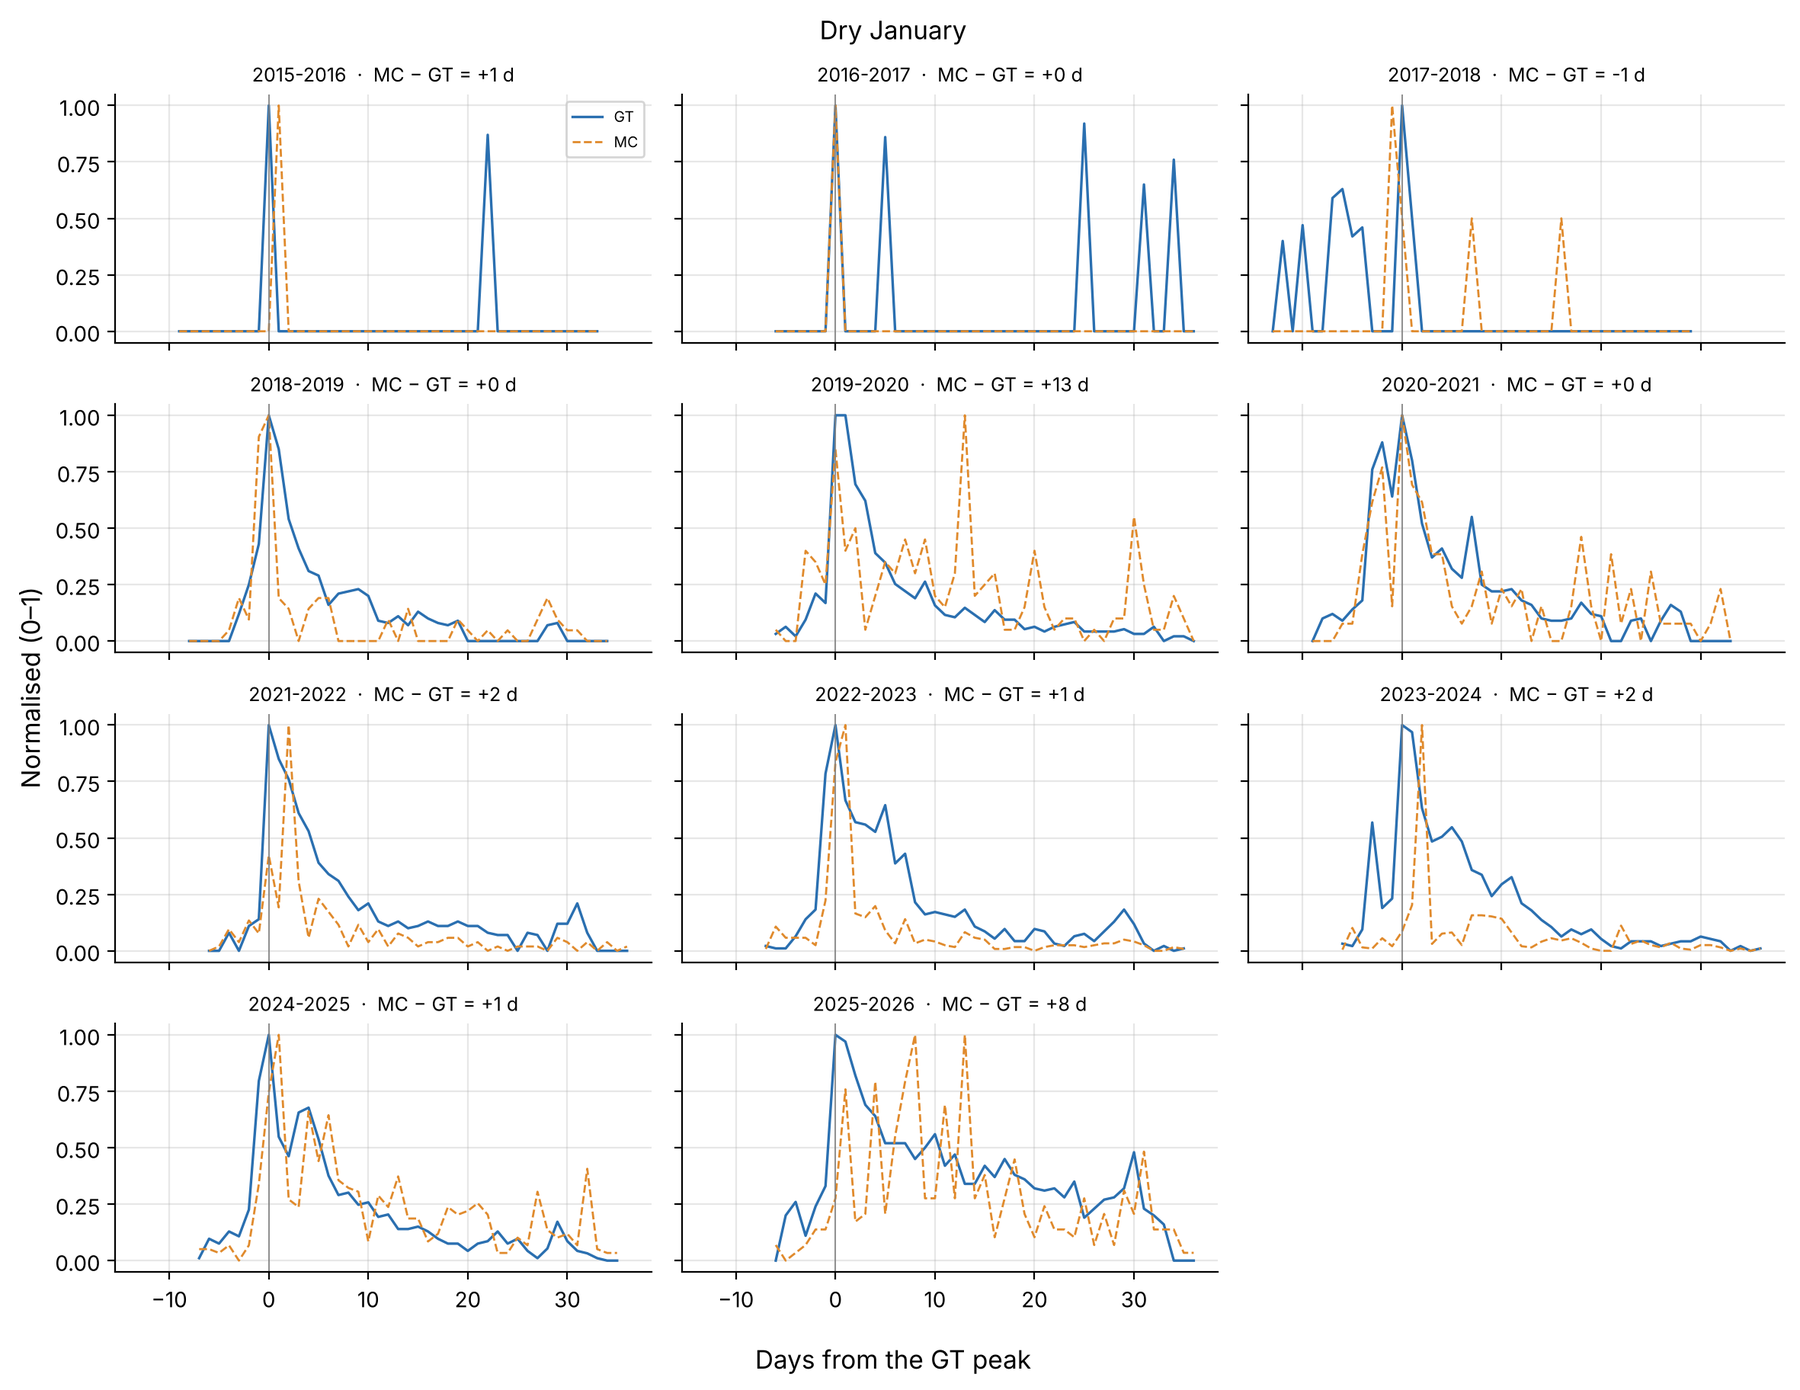
\includegraphics[width=\linewidth]{figure4-1.png}
        \caption{Dry January}
        \label{fig:peaks_dry_january}
    \end{subfigure}
    \hfill
    \begin{subfigure}{0.48\linewidth}
        \centering
        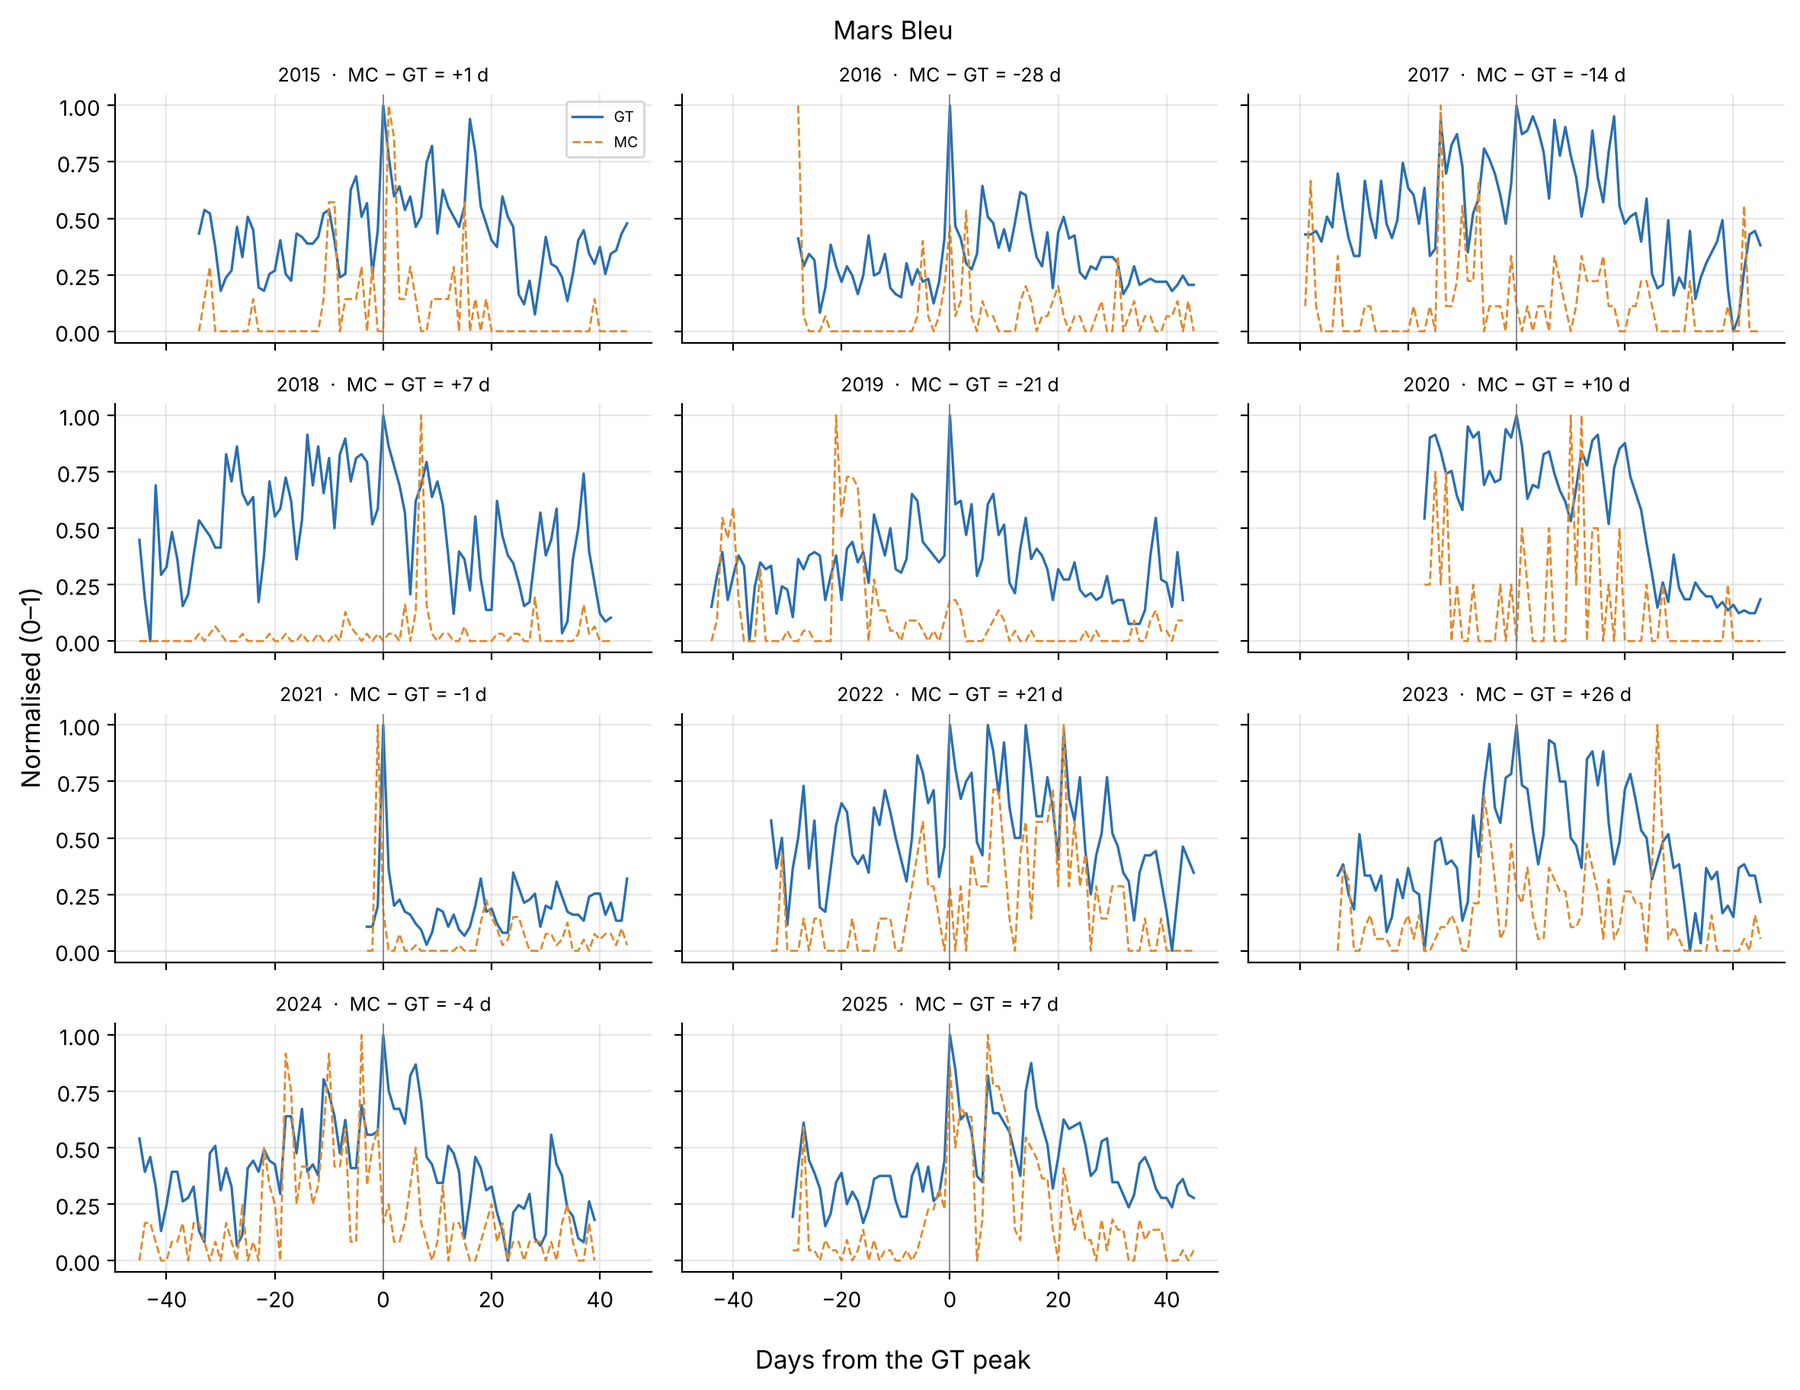
\includegraphics[width=\linewidth]{figure4-2.png}
        \caption{Mars Bleu}
        \label{fig:peaks_mars_bleu}
    \end{subfigure}

    \caption{Daily GT and MC series (min--max normalised to 0--1) aligned on the GT peak, by season, for (a) Dry January and (b) Mars Bleu.}
    \label{fig:peaks2}
\end{figure}

\subsection{Linear Granger causality}\label{sec:linear}
A series $X$ Granger-causes $Y$ if past values of $X$ improve the prediction of $Y$ beyond the information already contained in past values of $Y$ \cite{granger1969}. For the direction GT $\to$ MC we compare the unrestricted (full) and restricted (reduced) autoregressive models
\begin{align}
\text{full model:}\quad & MC_t = c + \sum_{k=1}^{p}\alpha_k MC_{t-k} + \sum_{k=1}^{q}\beta_k GT_{t-k} + \varepsilon_t,\\
\text{reduced model:}\quad & MC_t = c + \sum_{k=1}^{p}\alpha_k MC_{t-k} + \varepsilon_t,
\end{align}
estimated by ordinary least squares, and test the joint null hypothesis $H_0:\beta_1=\dots=\beta_q=0$. The direction MC $\to$ GT is obtained by exchanging the two series. With $n$ effective observations, the test statistic is
\begin{equation}
F=\frac{(RSS_{\mathrm{red}}-RSS_{\mathrm{full}})/q}{RSS_{\mathrm{full}}/(n-p-q-1)}\;\sim\;F(q,\,n-p-q-1)\ \text{under } H_0.
\end{equation}
Because statistical significance alone does not quantify the magnitude of the predictive relationship, we also report the incremental explanatory power as the gain in adjusted $R^2$:
\begin{equation}
\Delta R^2_{\mathrm{adj}} = R^2_{\mathrm{adj,full}} - R^2_{\mathrm{adj,red}},\qquad
R^2_{\mathrm{adj}} = 1-(1-R^2)\frac{n-1}{n-k-1},
\end{equation}
with $k=p$ for the reduced model and $k=p+q$ for the full model.

\paragraph{Within-season design.} Seasons are separated by several months, so a lagged value is only meaningful within the same campaign window. The lagged rows are therefore built inside each season, the first $\max(p,q)$ days of every season are dropped, and the seasons are then stacked. Without this precaution, the first days of each season are predicted from the last days of the previous year; this original specification is reported as a sensitivity analysis (Appendix~\ref{app:sensitivity}).

\paragraph{Lag selection.} The lag orders $(p^*,q^*)$ are selected separately for each campaign and direction by minimising the Akaike information criterion (AIC) \cite{akaike1974} of the full model over a $20\times20$ grid ($1\le p,q\le 20$), allowing asymmetric lag structures. Every cell of the grid is estimated on the same observations (from day 20 of each season), so that AIC values are comparable across lag orders (Figure~\ref{fig:aic}; all campaigns in Appendix~\ref{app:linfigs}).

\begin{figure}[htbp]
  \centering
  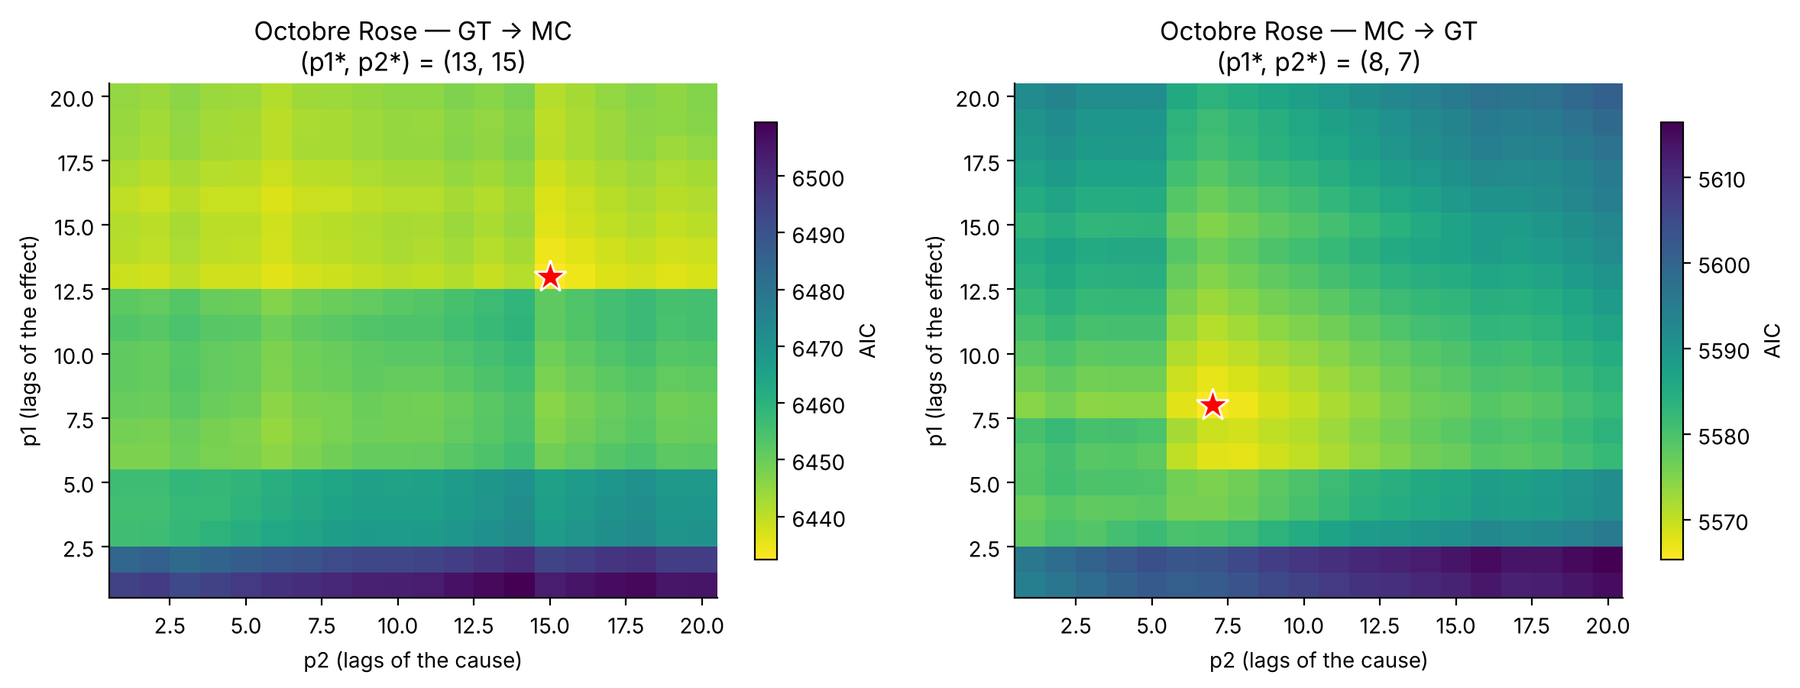
\includegraphics[width=\linewidth]{fig04_aic_octobre_rose}
  \caption{AIC of the full model as a function of the lag orders for Octobre Rose, GT $\to$ MC (left) and MC $\to$ GT (right), with within-season lags and a common sample. $p_1$ ($=p$): lags of the dependent variable; $p_2$ ($=q$): lags of the candidate cause. The star marks the AIC minimum.}
  \label{fig:aic}
\end{figure}

\paragraph{Inference and robustness.} The eight tests (four campaigns $\times$ two directions) are corrected for multiple testing with the Holm procedure \cite{holm1979}: the p-values are ranked, the smallest is multiplied by 8, the next by 7, and so on (never exceeding 1), which keeps the chance of at least one false positive among the eight tests below 5\%. Robustness is assessed by leave-one-year-out (LOYO) validation: each season is removed in turn and the test is re-estimated with the full-sample lags. Stationarity of each series is assessed with the augmented Dickey--Fuller (ADF) test \cite{dickey1979}, whose null hypothesis is a unit root, and the KPSS test \cite{kwiatkowski1992}, whose null hypothesis is stationarity.

\paragraph{Uncertainty and impulse responses.} The precision of $\Delta R^2_{\mathrm{adj}}$ is assessed with a delete-one-season jackknife: with $\hat\theta_{(i)}$ the gain estimated without season $i$ (the LOYO folds, $n=11$), $SE=\sqrt{\tfrac{n-1}{n}\sum_i(\hat\theta_{(i)}-\bar\theta)^2}$ and the 95\% interval is $\hat\theta\pm1.96\,SE$. A season bootstrap is not used for this statistic: drawing the same season twice inflates in-sample fit statistics, and in a first run the bootstrap intervals were shifted upwards. To express the predictive link in the units of the series, we compute the response of the effect to a one-off rise of 10 points in the cause (on the 0--100 within-season scale) from the fitted full model: $r_0=0$ and $r_t=\sum_{k}\alpha_k r_{t-k}+10\,\beta_t$ (with $\beta_t=0$ for $t>q$). These dynamic multipliers contain only lagged effects, as in the Granger test; their 95\% bands come from a season bootstrap (999 resamples, lags fixed), which is suitable here because they depend on regression coefficients rather than on in-sample fit.

\subsection{Accounting for the campaign calendar}\label{sec:calendar}
Granger tests assume that no unobserved variable drives both series. Here the campaign calendar does: it raises press coverage and searches on the same dates every year, which can produce significant tests in both directions without any day-to-day link between the series. We address this in two complementary ways.

\paragraph{Season-swap surrogates.} In plain terms: we pair the effect series of a season with the cause series of a different year (for instance the searches of 2022 with the coverage of 2019). If the real pairing predicts better than such mismatched pairings, the link holds from day to day and not only through the calendar both series share. Following the surrogate-data approach \cite{theiler1992}, the cause series of each season is replaced by the cause series of \emph{another} season (a random derangement of the seasons), aligned by day in the window. A surrogate keeps the cause's own dynamics and its campaign-shaped profile, but loses its day-to-day correspondence with the effect. The test statistic $\delta$, the share of the restricted model's unexplained variance captured by the cause, is computed for the real cause and for 199 surrogates, and the surrogate p-value is $p=(1+\#\{\delta_{\mathrm{surr}}\ge\delta_{\mathrm{obs}}\})/200$. To allow swaps, seasons are truncated to the length of the shortest season of the campaign. Surrogate p-values are Holm-adjusted across the eight campaign--direction pairs.

\paragraph{Calendar conditioning.} As a second variant, the day in the campaign window and the day of the week (as $\sin$ and $\cos$ of $2\pi d/7$) are added to both the restricted and unrestricted models, so that the cause must add information beyond a fixed calendar profile.

\paragraph{Calendar adjustment of the series.} A season-swap surrogate keeps the campaign profile but not the weekly cycle (a given date falls on a different weekday from one year to the next), and it leaves untouched the differences of level between seasons. We therefore repeat the surrogate tests, with 999 surrogates (smallest attainable $p=0.001$), after five adjustments of both series: (A) none; (B) the day-of-week effect removed (estimated jointly with the profile and the season levels); (C) the mean of each season removed; (D) the campaign profile (average over seasons for each calendar date) and the day-of-week effect removed, season levels kept; (E) all three removed (the anomalies of Section~\ref{sec:tf}). A further surrogate scheme that shifts the donor season by up to three days so that weekdays coincide is reported in the appendix. The adjustments are estimated on the real series; the surrogates swap the adjusted cause.

\subsection{Nonlinear Granger causality}\label{sec:nonlinear}
Linear tests miss relationships without linear correlation, such as threshold effects. We use the two constraint-based kernel methods reviewed and unified by Murphy and Benavoli \cite{murphy2026}. Let $y$ be the effect at day $t$, $X$ its past values (restricted inputs), $X_a$ the past values of the cause, and $Z=[X,X_a]$; series are standardised.

\paragraph{Kernel Granger causality (KGC).} KGC \cite{marinazzo2008} performs linear Granger causality in the feature space of a kernel. With the centred kernel matrix $K(X,X)$, let $P$ be the projector on its range; the part of $y$ that its own past cannot explain is $e=(I-P)y$. The new directions brought by the cause are the eigenvectors $w_i$ of $\tilde K=(I-P)K(Z,Z)(I-P)$. With $r_i=\mathrm{corr}(e,w_i)$, the original index sums $r_i^2$ over the correlations that are significant after Bonferroni correction, and $\delta=\sum_i r_i^2$ is used for the permutation test of Section~\ref{sec:calendar}. That test, which permutes whole seasons, is the one on which we base our conclusions for all three nonlinear and linear methods; the parametric test of the original method (Student $t$ with Bonferroni correction) is computed for comparison (Appendix Figure~\ref{fig:main}). We use a squared-exponential kernel with the lengthscale heuristic of \cite{murphy2026}, and a polynomial kernel of degree 1, with which KGC reduces exactly to linear Granger causality.

\paragraph{Large-scale nonlinear Granger causality (lsNGC).} lsNGC \cite{wismuller2021} places $c_f=25$ k-means centres in the space of $X$ and $c_g=5$ in the space of $X_a$, maps each observation to normalised Gaussian activations around these centres, and compares least-squares fits of $y$ on $f(X)$ and on $[f(X),g(X_a)]$ with an F-test; $\delta=1-SSR_u/SSR_r$ is used for the surrogate test. For both methods, the precision of $\delta$ is assessed with the delete-one-season jackknife, and its chance level is given by the mean over surrogates. Because lsNGC places its centres with k-means, whose result depends on a random initialisation, its tests are repeated with 10 seeds.

\paragraph{Lag order.} For each campaign and direction, the lag order $m\in\{1,2,3,5,7\}$ is chosen from the effect's \emph{own} past only, by leave-one-season-out cross-validation of a kernel ridge model, so that the choice cannot favour finding a link (Appendix Figure~\ref{fig:lagsel}). Lags are kept within each season. The parametric tests of the original papers are reported for comparison, with Holm correction for KGC and Benjamini--Hochberg control of the false discovery rate for lsNGC, as in their original papers.

\subsection{Transfer functions}\label{sec:tf}
Granger tests ask \emph{whether} the past of one series improves the prediction of the other. They do not say how large the response is, when it arrives, or how long it lasts. A transfer function \cite{box2015} describes the response of an output $y$ to an input $x$,
\begin{equation}
y_t = c + \sum_{k\ge0}\nu_k\,x_{t-k} + N_t,\qquad \phi(B)\,N_t=e_t,
\end{equation}
where $\nu_k$ is the response of $y$, $k$ days later, to a rise of one point in $x$ lasting one day, $B$ is the backshift operator and $N_t$ is an AR($p$) noise ($p\le7$, chosen by AIC on the output's own past so that it cannot depend on the input). We estimate it for GT $\to$ MC and for MC $\to$ GT by conditional least squares, within seasons.

\paragraph{Calendar removal.} Fitted to raw series, a transfer function would attribute the shared campaign profile and the weekly cycle to the other series. Each series is first split by least squares into a date profile (one level per calendar date, the average campaign shape over the 11 seasons), a day-of-week effect, a season level and an \emph{anomaly}; the transfer function is estimated on the anomalies. It therefore describes how day-to-day departures of one series from its usual campaign shape are followed by departures of the other. The profile, the weekly term and the season level are re-estimated in every jackknife replicate (below); for the surrogates the anomalies are computed once, so that a surrogate input has no calendar component left.

\paragraph{Same-day and lagged responses.} With daily data, the same-day weight $\nu_0$ is a correlation without direction: it is the same whichever series is called the input, and it is the only coefficient that two series driven by the same event on the same day would produce. The lagged weights $\nu_1,\nu_2,\dots$ do have a direction, and stay correctly estimated when the series influence each other, because the past of the input cannot depend on today's noise. We therefore report $\nu_0$ and the lagged response $\sum_{k=1}^{14}\nu_k$ separately.

\paragraph{Two parametrisations.} (i) A \emph{distributed lag} leaves $\nu_0,\dots,\nu_{14}$ free. (ii) A \emph{delay-and-decay} model imposes $\nu(B)=\omega B^{b}/(1-\delta B)$, i.e.\ $\nu_k=\omega\,\delta^{\,k-b}$ for $k\ge b$ and $0$ before. Three numbers summarise it: the delay $b$ (chosen among 0--7 days by AIC), the total gain $\omega/(1-\delta)$ (response to a sustained one-point rise) and the half-life $\ln(1/2)/\ln\delta$. The share of the output's unpredicted variance (what its own AR model leaves) explained by the input at lags 1--14, beyond the same-day term, is reported as $R^2_{\mathrm{lag}}$. Box--Jenkins diagnostics (Ljung--Box test of the residuals; cross-correlation of the residuals with the pre-whitened input) are given in the notebook; their $p$-values treat days as independent and are indicative only.

\paragraph{Identification without a model.} The input is filtered by its own AR model (pre-whitening) and the same filter is applied to the output; the cross-correlation of the two filtered series at lag $k$ is then proportional to $\nu_k$. Negative lags show the output leading the input, i.e.\ feedback, which the single-input model excludes. Bands come from season-swap surrogates (999), and a simultaneous band, the level exceeded at any of the 29 lags by 5\% of the surrogates, accounts for looking at many lags.

\paragraph{Inference.} The season is the unit of replication. Standard errors and 95\% intervals come from the delete-one-season jackknife (Student $t$, 10 degrees of freedom), with the noise order and the delay re-selected in each replicate. $P$-values come from 999 season-swap surrogates: the anomalies of the input of each season are replaced by those of another season, the delay is re-selected for every surrogate, and three statistics are compared with their surrogate distribution: the gain in $R^2$ from lags 1--14 (one-sided; ``lagged fit''), the lagged response $\sum_{k=1}^{14}\nu_k$ (two-sided; ``lagged sum'') and $\nu_0$ (two-sided). They are Holm-adjusted across the eight campaign--direction pairs.

\paragraph{Frequency domain.} The same question by period. With one Hann-tapered segment per season, the squared coherence at a frequency is the share of the variance of one series linearly related to the other, and the phase gives their delay. With 11 seasons, two unrelated series exceed a squared coherence of 0.26 at a given frequency 5\% of the time ($1-0.05^{1/10}$).

\subsection{Checks on simulated data}\label{sec:simulation}
On real data the truth is unknown, so we cannot tell whether a test finds links that exist and avoids inventing links that do not. We therefore first run every test on artificial data in which we chose the truth. A \emph{dataset} here is one artificial copy of the study: 11 seasons of 91 days of two series generated by a known rule, with fresh random noise each time. Repeating this 100 times for each scenario gives the share of datasets in which a test declares a link. The tests are run on four such systems, with 39 surrogates per test; rejection rates are reported with 95\% Wilson intervals: (a) a purely nonlinear link, where GT depends on the square of the previous day's MC, so that the two series have no linear correlation; (b) two independent series; (c) a common driver with fixed timing, a campaign pulse on the same days every year driving both series, with no direct link; and (d) a common driver whose timing varies by up to $\pm15$ days from year to year, again with no direct link. The transfer-function procedure is checked separately on systems in which GT acts on MC through a known transfer function ($\nu_k=0.5\times0.6^{k-1}$ for $k\ge1$: delay one day, response cumulated over 14 days 1.249, half-life 1.36 days) on top of a campaign pulse and a weekly cycle shared by both series: (e) with this link only; (f) with the link and a feedback of MC on GT ($\nu_k=0.15\times0.5^{k-1}$, cumulated response 0.300); (g) with no link and a fixed calendar; (h) with no link and a campaign pulse whose timing varies by up to $\pm15$ days. There are 100 datasets per scenario and 99 surrogates per test. Finally, to check whether a weekly cycle shared by both series makes the surrogate tests find links, system (c) is given a shared weekly cycle (a weekend dip of 0.7 for MC and 0.42 for GT relative to working days, i.e.\ 7\% of the variance of the AR(1) noise for MC; the weekly term carries 0.2--9\% of the variance of the real series, Appendix Figure~\ref{fig:tfcal}) and the tests are run under adjustments (A) and (B), and with weekday-aligned surrogates (100 datasets, 39 surrogates).

% ==================================================================
\section{Results}
% ==================================================================
\subsection{Temporal alignment of media and search peaks}
All four campaigns exhibit a sharp annual GT peak during the campaign month (Figure~\ref{fig:overview}). For Dry January, search interest is almost absent before 2019 and increases steadily thereafter. Table~\ref{tab:peaklag} summarises the lag between the MC and GT peaks. Peaks are synchronous for Octobre Rose and Dry January (lag within $\pm2$ days in 9 of 11 seasons), whereas for Movember the media peak follows the search peak in most seasons (median $+9$ days), and Mars Bleu shows no stable alignment.

\begin{table}[htbp]
\centering
\caption{Lag between the MC peak and the GT peak (days; positive = media peak after search peak), read from Figures~\ref{fig:peaks1}--\ref{fig:peaks2}. 11 seasons per campaign.}
\label{tab:peaklag}
\begin{tabular}{lccc}
\toprule
Campaign & Median & Range & Seasons with $|\text{lag}|\le 2$ \\
\midrule
Octobre Rose & 0  & $-2$ to $+10$  & 9/11 \\
Dry January  & +1 & $-1$ to $+13$  & 9/11 \\
Movember     & +9 & $-11$ to $+47$ & 0/11 \\
Mars Bleu    & +1 & $-28$ to $+26$ & 2/11 \\
\bottomrule
\end{tabular}
\end{table}

\subsection{Stationarity}
The ADF test rejects a unit root for all eight series ($p<0.001$). The KPSS test nevertheless rejects stationarity at the 5\% level for Dry January (GT and MC), Octobre Rose (GT) and Mars Bleu (MC) (Appendix~\ref{app:stationarity}). Together, the two tests indicate no unit root but a non-constant mean, as expected from series that form a pulse around each campaign; for Dry January, the near absence of searches before 2019 adds a trend across seasons.

\subsection{Linear Granger causality}
Table~\ref{tab:granger} reports the linear tests with within-season lags. In the GT $\to$ MC direction, past searches improve the prediction of press coverage for Mars Bleu, Movember and Octobre Rose (Holm-adjusted $p<10^{-7}$, all 11 LOYO folds significant), with $\Delta R^2_{\mathrm{adj}}$ between 0.034 and 0.073. For Dry January the link is absent ($p=0.27$, no significant LOYO fold). In the MC $\to$ GT direction, the tests are significant after correction for Dry January, Movember and Octobre Rose, but not for Mars Bleu ($p=0.42$). The effect sizes in this direction are small: GT is strongly autoregressive, its own past already explaining 50\% (Dry January) to 82\% (Octobre Rose) of its variance, and adding past media coverage raises the adjusted $R^2$ by at most 0.022.

Compared with the original specification, in which lags cross the boundary between seasons, two links disappear: Dry January GT $\to$ MC and Mars Bleu MC $\to$ GT (Appendix~\ref{app:sensitivity}). Part of the significance of these tests came from rows that predicted the start of a season from the end of the previous year. Figure~\ref{fig:r2} compares the adjusted $R^2$ of the reduced and full models; the estimated coefficients are given in Appendix~\ref{app:linfigs}.

The jackknife intervals (Table~\ref{tab:granger}) confirm that the GT $\to$ MC gains are clearly positive for Mars Bleu, Movember and Octobre Rose. In the MC $\to$ GT direction, the gains are tiny and their intervals include zero for Dry January ($-0.022$ to 0.067) and Octobre Rose ($-0.0003$ to 0.0076), despite very small p-values: these links depend on a few seasons.

\paragraph{Impulse responses.} Figure~\ref{fig:irf} expresses the links in points of the 0--100 within-season scale. After a one-off rise of 10 points in searches, press coverage increases by 5.6 to 7.7 points summed over the following 14 days for Mars Bleu, Movember and Octobre Rose (95\% intervals from 2.8 to 10.3), with a weekly zigzag that reflects the publication cycle of the press. In the MC $\to$ GT direction the responses are small and, for Movember and Octobre Rose, \emph{negative}: a rise of 10 points in coverage is followed by searches lower by 4.5 (Movember, interval $-6.7$ to $-2.6$) and 3.3 points (Octobre Rose, $-7.2$ to $-0.1$) over 14 days. Only Dry January shows a positive response (4.4 points, 0.1 to 7.3). The significant linear MC $\to$ GT tests therefore do not describe coverage raising searches. For Movember, this agrees with the media peak following the search peak by about nine days (Table~\ref{tab:peaklag}): coverage tends to be high when searches are already declining.

\begin{figure}[htbp]
  \centering
  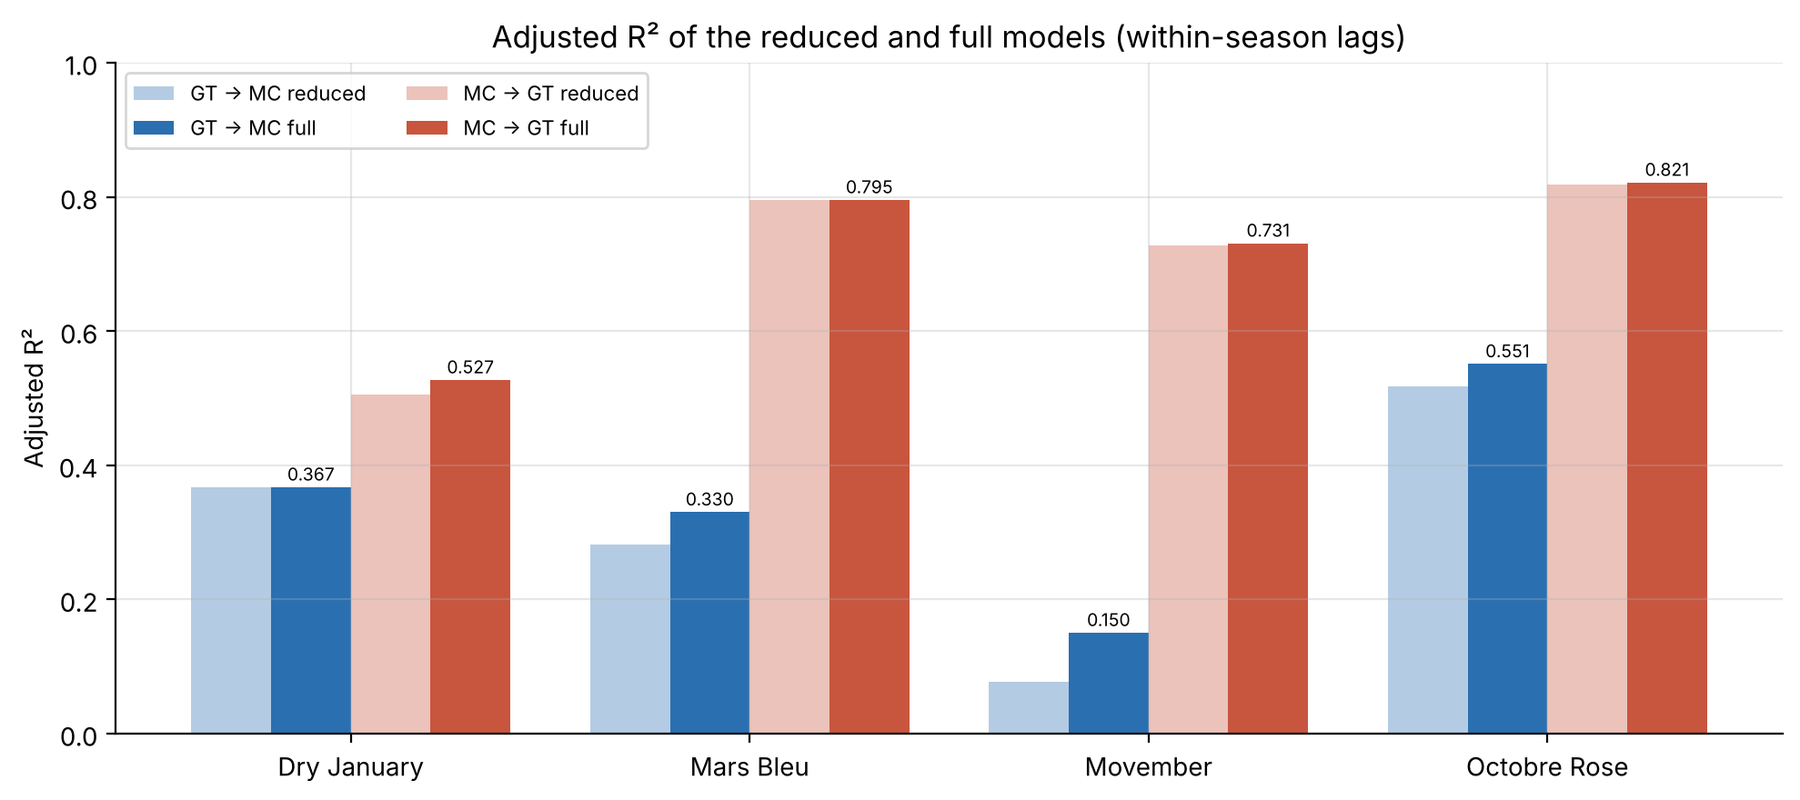
\includegraphics[width=\linewidth]{fig05_adjusted_r2}
  \caption{Adjusted $R^2$ of the reduced (light) and full (dark) models for each campaign, GT $\to$ MC (blue) and MC $\to$ GT (red), with within-season lags.}
  \label{fig:r2}
\end{figure}

\begin{figure}[htbp]
  \centering
  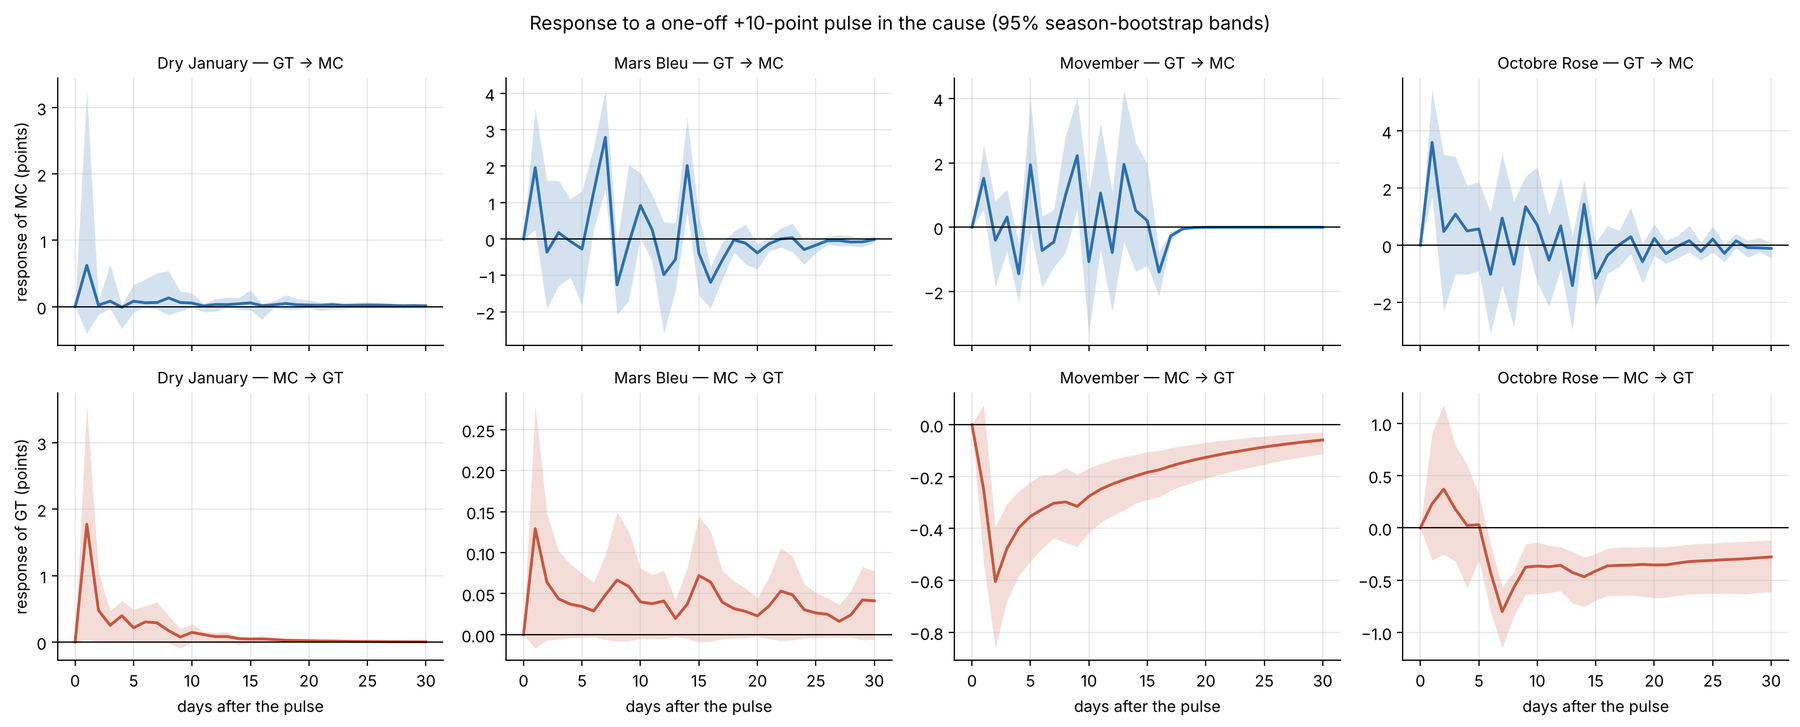
\includegraphics[width=\linewidth]{fig13_impulse_responses}
  \caption{Response of the effect to a one-off rise of 10 points in the cause, from the linear full models (top: GT $\to$ MC; bottom: MC $\to$ GT), with 95\% season-bootstrap bands (999 resamples). Units: points of the 0--100 within-season scale.}
  \label{fig:irf}
\end{figure}

\subsection{Robustness (LOYO)}
The leave-one-year-out folds confirm the full-sample results (Figures~\ref{fig:loyo-p}--\ref{fig:loyo-mcgt}). In the GT $\to$ MC direction, every fold is significant for Mars Bleu, Movember and Octobre Rose (largest fold p-value $2.3\times10^{-6}$, $5.4\times10^{-8}$ and $2.1\times10^{-7}$ respectively), and none is for Dry January. In the MC $\to$ GT direction, every fold is significant for Movember and Octobre Rose, although the Movember p-values are closer to the threshold (largest $0.024$); for Dry January, only the fold without the 2017--2018 season is not significant ($p=0.073$); for Mars Bleu, no fold is significant. The mean $\Delta R^2_{\mathrm{adj}}$ across folds stays within 0.001 of its full-sample value for every campaign and direction.

\begin{figure}[htbp]
  \centering
  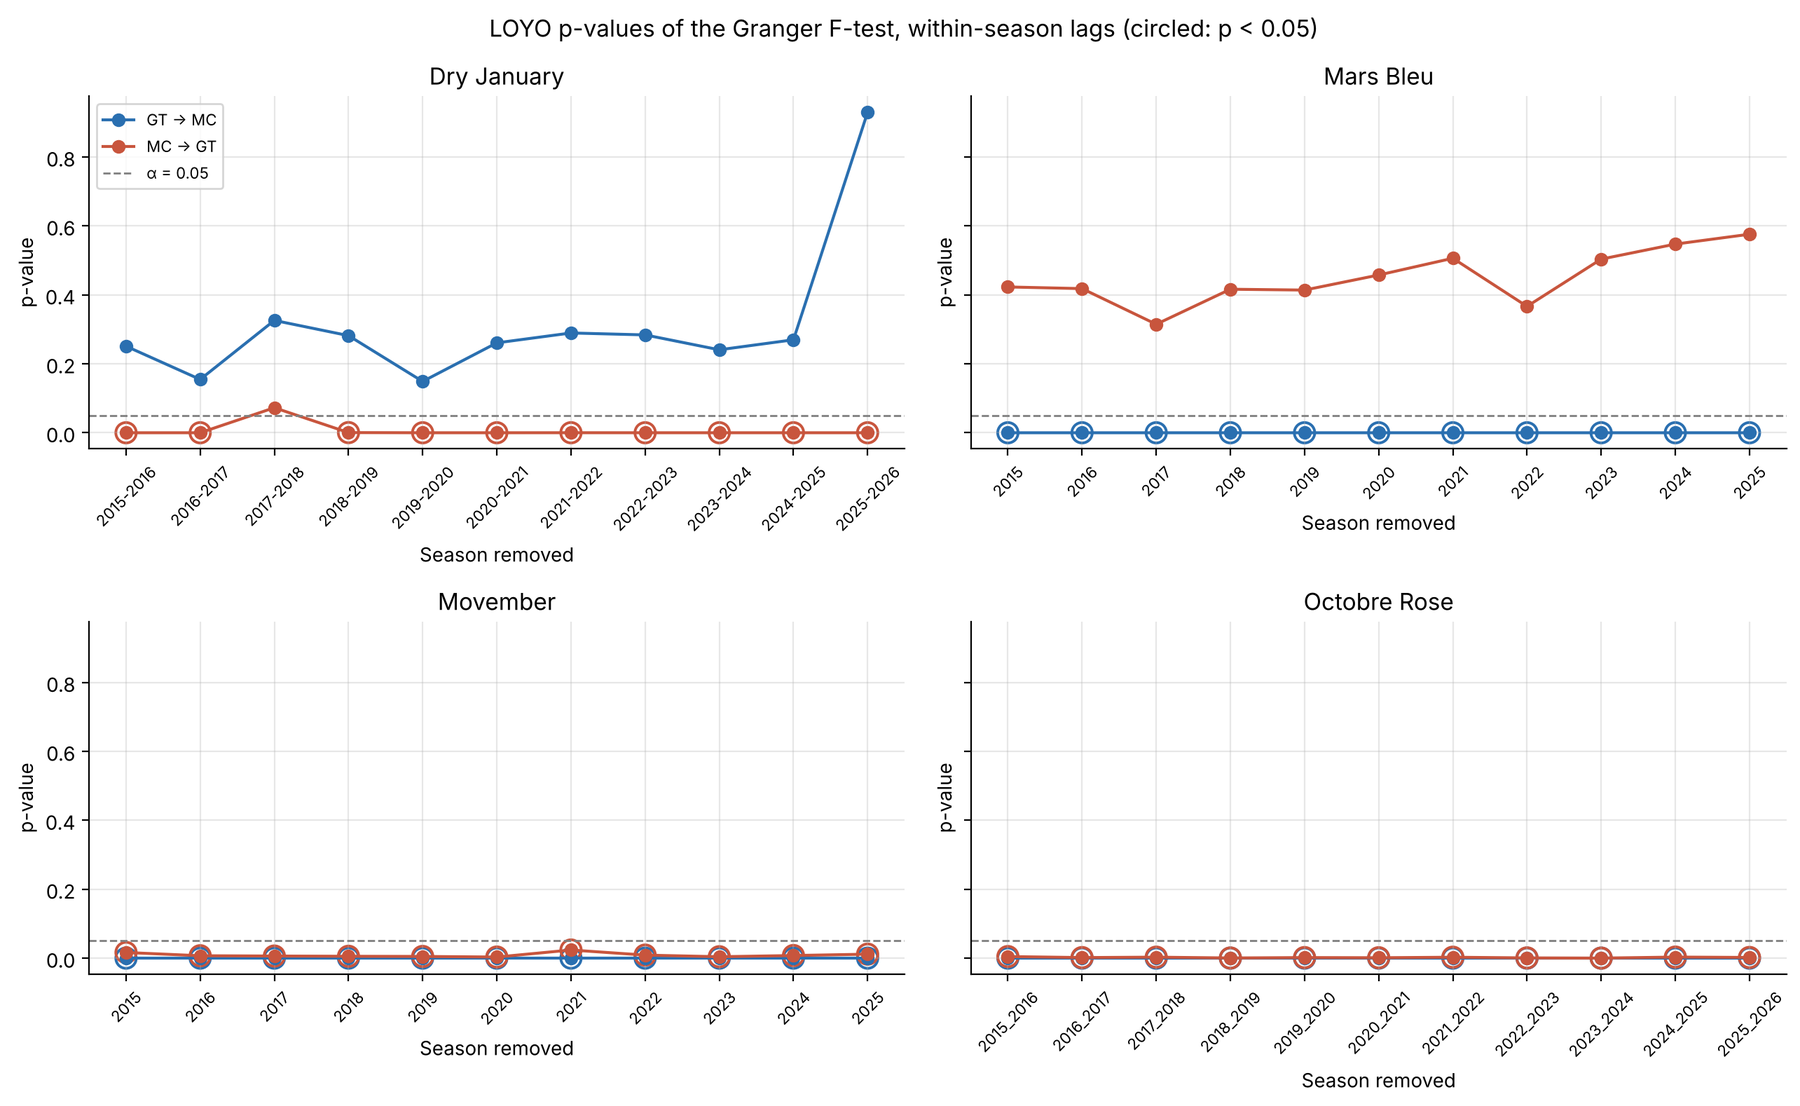
\includegraphics[width=\linewidth]{fig06_loyo_pvalues}
  \caption{LOYO p-values of the linear Granger F-test with within-season lags, GT $\to$ MC (blue) and MC $\to$ GT (red), by excluded season. Circled points are significant ($p<0.05$); dashed line: 0.05.}
  \label{fig:loyo-p}
\end{figure}

\begin{figure}[htbp]
  \centering
  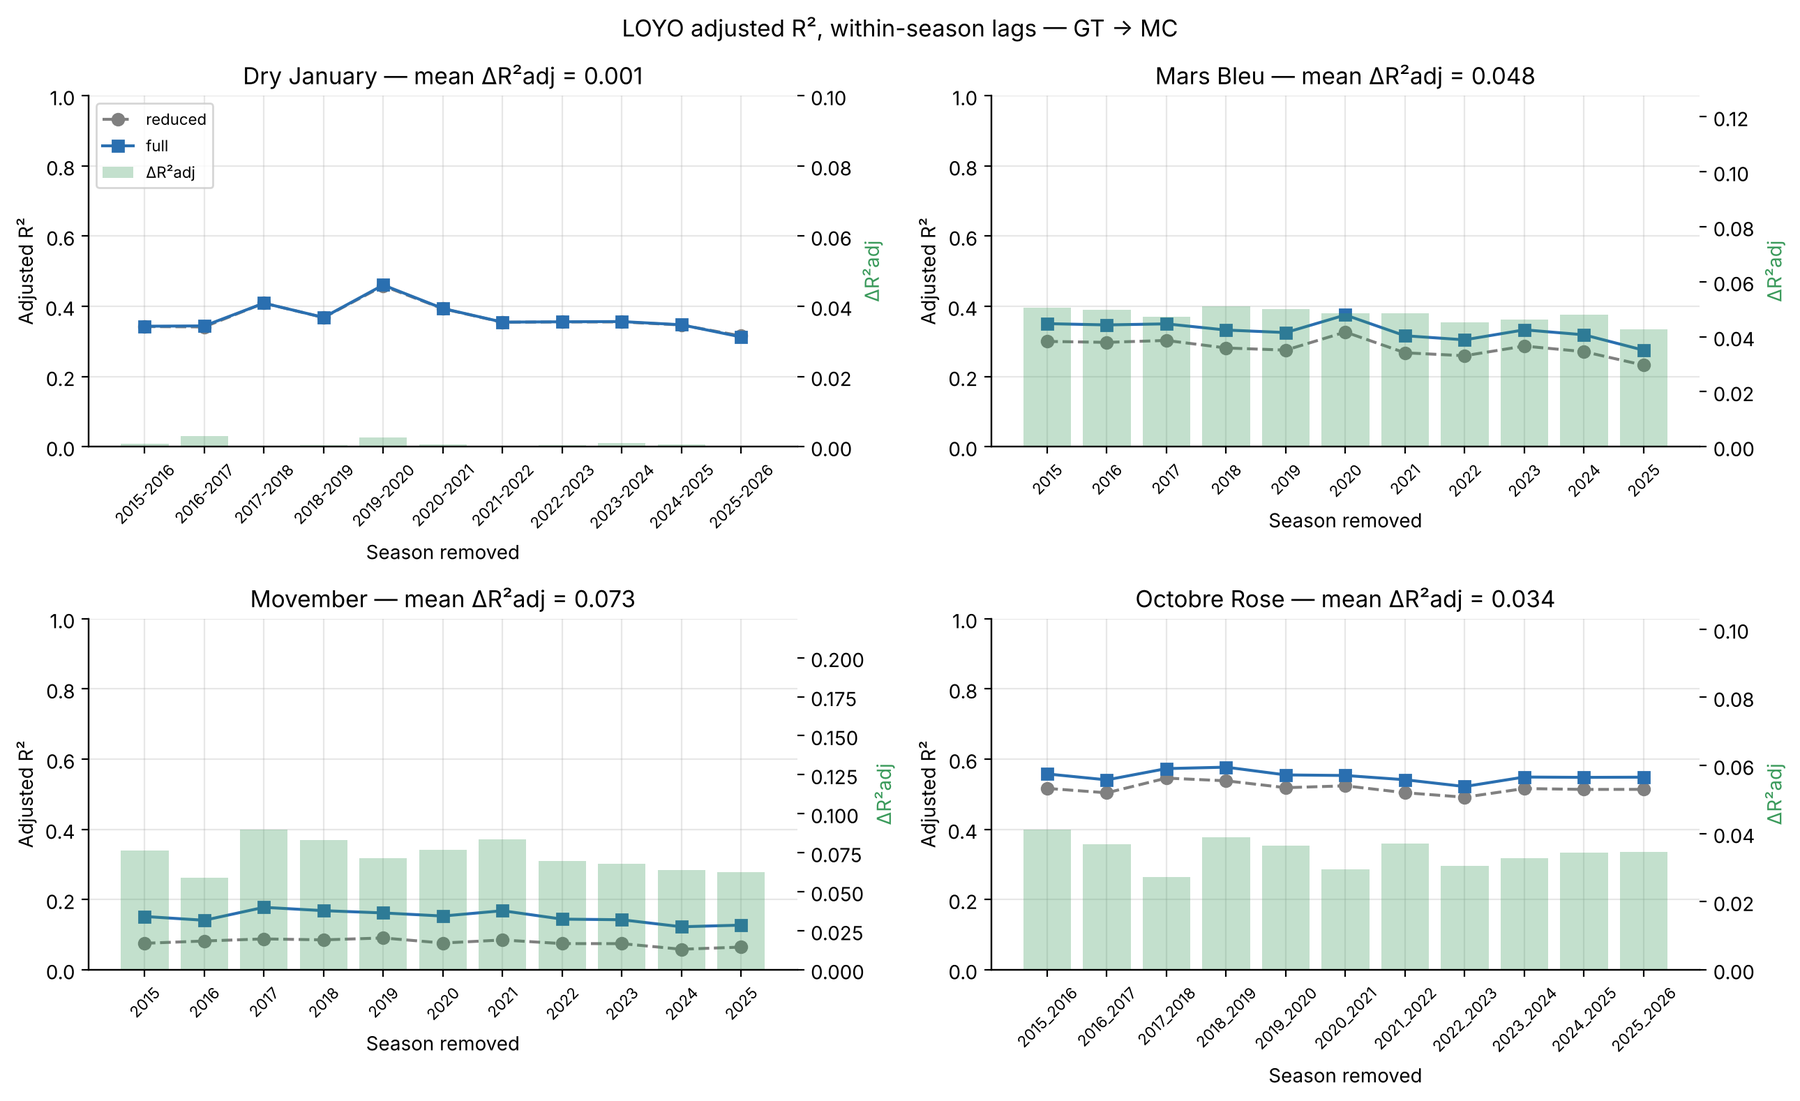
\includegraphics[width=\linewidth]{fig07_loyo_r2_gt_to_mc}
  \caption{LOYO adjusted $R^2$ for GT $\to$ MC: reduced model (grey), full model (blue) and $\Delta R^2_{\mathrm{adj}}$ (green bars, right axis), by excluded season.}
  \label{fig:loyo-gtmc}
\end{figure}

\begin{figure}[htbp]
  \centering
  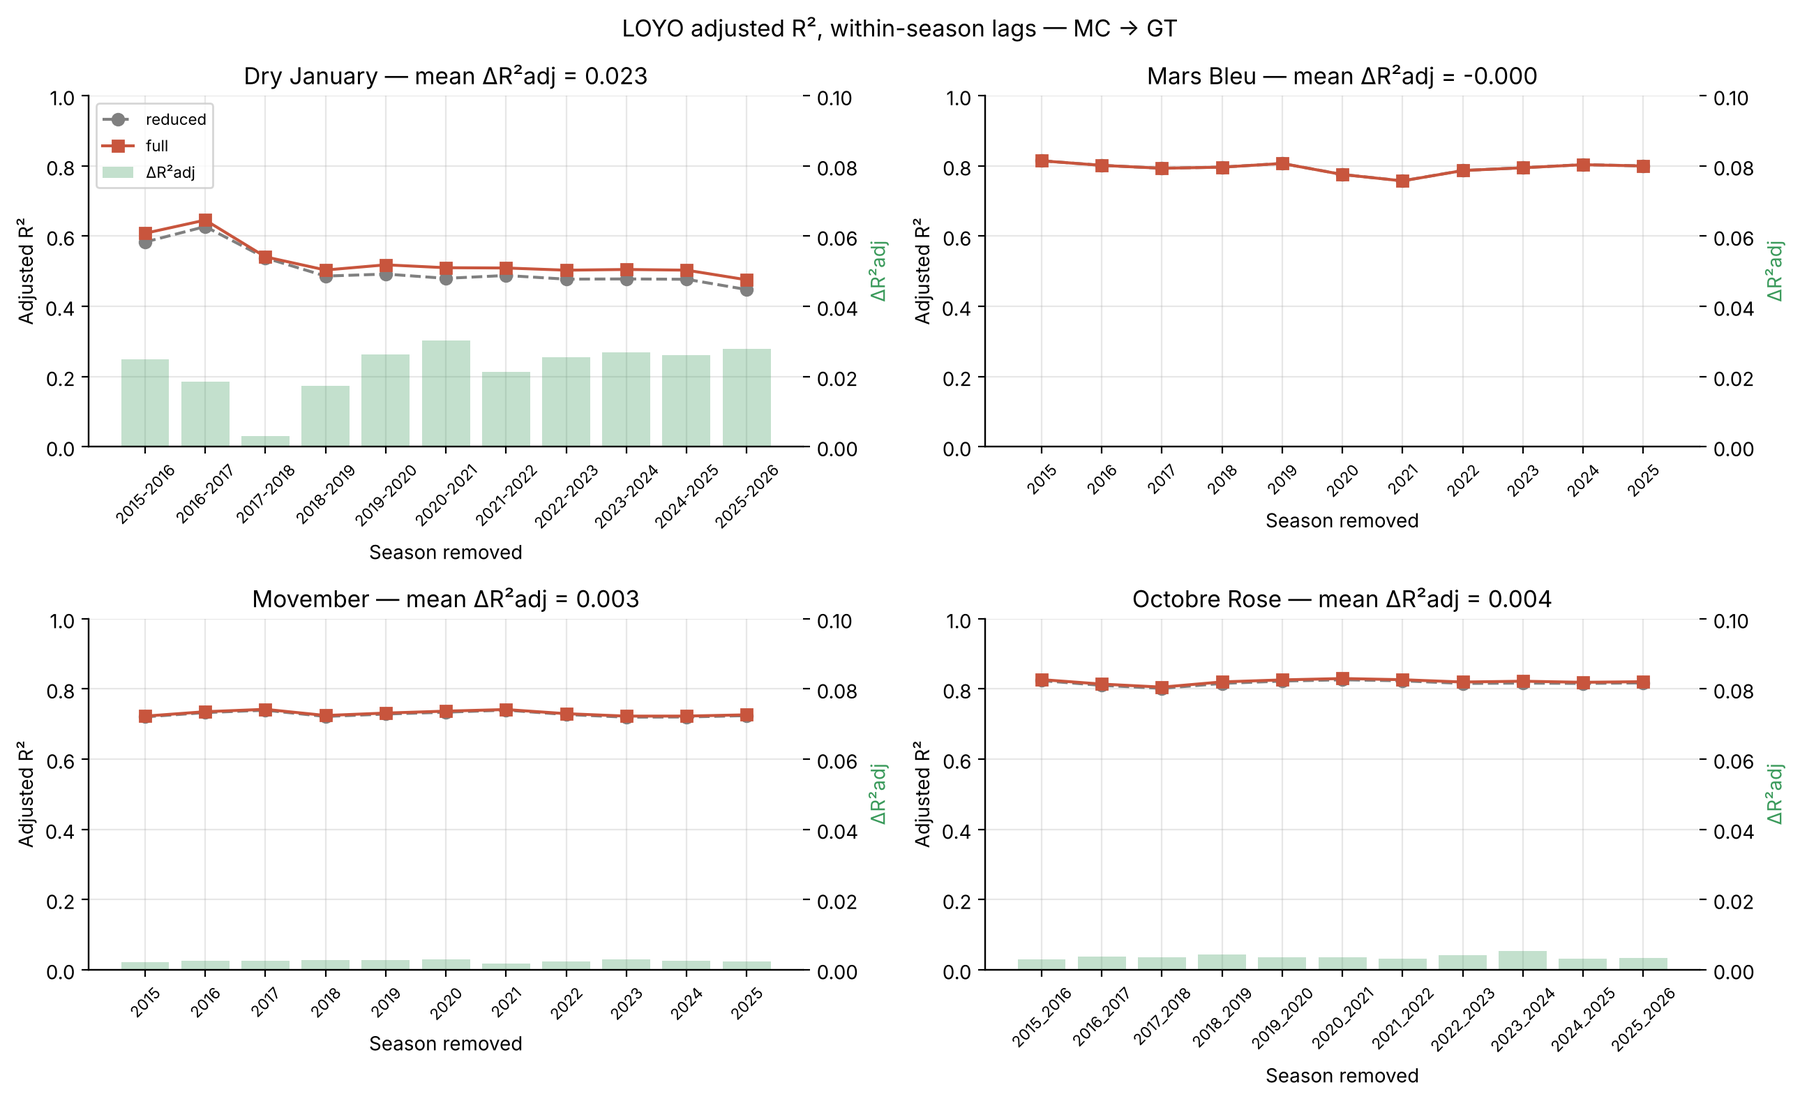
\includegraphics[width=\linewidth]{fig08_loyo_r2_mc_to_gt}
  \caption{LOYO adjusted $R^2$ for MC $\to$ GT. The reduced and full curves almost overlap, reflecting the strong autoregressive persistence of GT.}
  \label{fig:loyo-mcgt}
\end{figure}

\begin{table}[htbp]
\centering
\caption{Linear Granger causality with within-season lags. $p^*$: lags of the dependent variable; $q^*$: lags of the candidate cause (AIC on a common sample); $n$: number of predicted days. $\Delta R^2_{\mathrm{adj}}$ with its 95\% delete-one-season jackknife interval. $p_{\mathrm{Holm}}$: Holm-adjusted across the eight tests. LOYO: number of leave-one-year-out folds with $p<0.05$.}
\label{tab:granger}
\footnotesize
\setlength{\tabcolsep}{3.5pt}
\resizebox{\linewidth}{!}{%
\begin{tabular}{llccccccccc}
\toprule
Campaign & Direction & $(p^*,q^*)$ & $n$ & $R^2_{\mathrm{adj,red}}$ & $R^2_{\mathrm{adj,full}}$ & $\Delta R^2_{\mathrm{adj}}$ & 95\% CI & p-value & $p_{\mathrm{Holm}}$ & LOYO \\
\midrule
Dry January  & GT $\to$ MC & (18, 1)  & 275 & 0.367 & 0.367 & 0.0005    & [$-0.008$, 0.009]     & 0.27                & 0.55                & 0/11 \\
             & MC $\to$ GT & (9, 1)   & 374 & 0.505 & 0.527 & 0.0223    & [$-0.022$, 0.067]     & $2.6\times10^{-5}$  & $1.3\times10^{-4}$  & 10/11 \\
Mars Bleu    & GT $\to$ MC & (10, 16) & 795 & 0.282 & 0.330 & 0.0480    & [0.033, 0.063]        & $1.2\times10^{-8}$  & $7.0\times10^{-8}$  & 11/11 \\
             & MC $\to$ GT & (17, 1)  & 784 & 0.796 & 0.795 & $-0.0001$ & [$-0.0005$, 0.0003]   & 0.42                & 0.55                & 0/11 \\
Movember     & GT $\to$ MC & (1, 16)  & 836 & 0.078 & 0.150 & 0.0726    & [0.015, 0.130]        & $3.7\times10^{-11}$ & $3.0\times10^{-10}$ & 11/11 \\
             & MC $\to$ GT & (8, 2)   & 924 & 0.728 & 0.731 & 0.0025    & [0.0002, 0.0049]      & $5.0\times10^{-3}$  & $1.5\times10^{-2}$  & 11/11 \\
Octobre Rose & GT $\to$ MC & (13, 15) & 836 & 0.517 & 0.551 & 0.0338    & [0.009, 0.059]        & $8.5\times10^{-10}$ & $6.0\times10^{-9}$  & 11/11 \\
             & MC $\to$ GT & (8, 7)   & 913 & 0.818 & 0.821 & 0.0036    & [$-0.0003$, 0.0076]      & $7.4\times10^{-4}$  & $3.0\times10^{-3}$  & 11/11 \\
\bottomrule
\end{tabular}}
\end{table}

\subsection{Checks on simulated data}
Figure~\ref{fig:simulation} shows how often each test declares a link in 100 simulated datasets per scenario (p-values for one dataset per scenario in Appendix Figure~\ref{fig:simsingle}). KGC and lsNGC detect the purely nonlinear MC $\to$ GT link in all 100 datasets, with or without surrogates, whereas linear Granger causality detects it in only 27--29. When there is no link (independent series, and the GT $\to$ MC direction of the nonlinear system), every test declares a link in 0--7\% of the datasets, consistent with the nominal 5\% level given the simulation uncertainty (with 100 datasets, a true rate of 5\% is observed between about 2\% and 11\%). Under a common driver with fixed timing, the standard tests report spurious links in 39--100\% of the datasets; with season-swap surrogates this drops to 4--7\%. Under a common driver whose timing varies across years, all tests, surrogate tests included, still report spurious links (32--94\% of the datasets). Standard Granger tests are therefore not interpretable on campaign data; surrogate tests remove the effect of a fixed calendar, but not that of events whose date changes from year to year.

\begin{figure}[htbp]
  \centering
  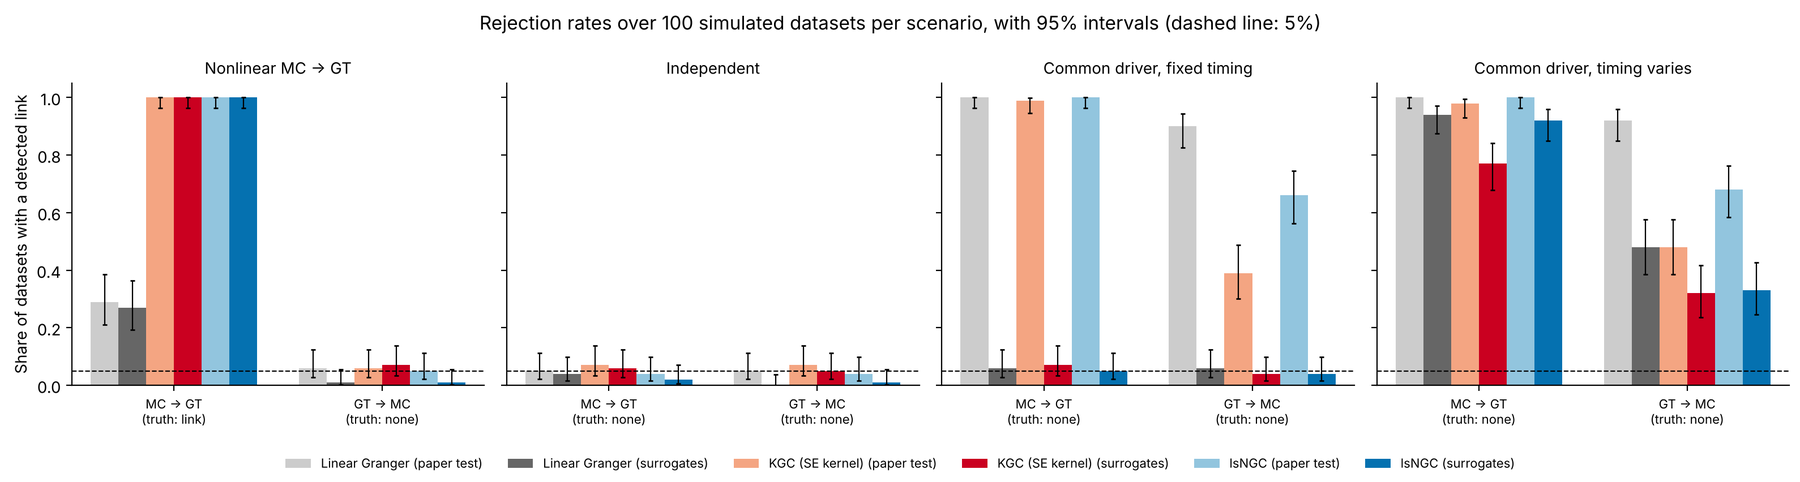
\includegraphics[width=\linewidth]{kg02_simulation_rates}
  \caption{Share of 100 simulated datasets in which each test declares a link, for four systems with a known truth, with 95\% Wilson intervals (dashed line: 5\%). ``Paper test'': parametric test of the original method; ``surrogates'': season-swap surrogate test (39 surrogates).}
  \label{fig:simulation}
\end{figure}

\subsection{Links beyond the campaign calendar}
Table~\ref{tab:surrogates} reports the surrogate tests on campaign data, and Appendix Figure~\ref{fig:main} compares them with the standard tests. Without accounting for the calendar, at least one of the three standard tests is significant for 7 of the 8 campaign--direction pairs (all except Mars Bleu MC $\to$ GT), a pattern that the simulations show a shared calendar alone can produce.

Against season-swap surrogates, one link survives correction for multiple testing within the family of eight tests: \textbf{Movember, MC $\to$ GT}, with lsNGC (unadjusted $p=0.005$, the real coverage series beating all 199 surrogates; Holm-adjusted $p=0.040$). It does so for all 10 k-means initialisations of lsNGC ($\delta$ between 0.024 and 0.028, $p=0.005$ each time; Appendix Table~\ref{tab:seeds}). The effect is small: media coverage explains 2.7\% of the variance of searches left unexplained by their own past (jackknife 95\% interval 0.9\% to 4.4\%), against 0.6\% on average for surrogates (Appendix Figures~\ref{fig:null}--\ref{fig:jkdelta}). The link is robust to the lag order: with lsNGC it holds at every order from 1 to 7 days, and KGC with a squared-exponential kernel gives surrogate p-values of 0.025 at 5 and 7 days but not at 2 days ($p=0.30$; Appendix Figure~\ref{fig:lagsens}). With calendar conditioning the link points in the same direction but no longer survives correction (unadjusted $p=0.015$, adjusted $p=0.12$).

\paragraph{Which part of the calendar does the link depend on?} Table~\ref{tab:adjust} repeats the lsNGC tests with 999 surrogates after the five adjustments of Section~\ref{sec:calendar}. The Movember link is unchanged by removing the weekly cycle or the season means (Holm-adjusted $p=0.008$, the smallest attainable, in variants A, B and C); the statistic falls from 0.027 to 0.018 when the weekly cycle is removed (chance level 0.006), and 8 of 10 k-means initialisations remain significant after correction (10 of 10 with weekday-aligned surrogates; Appendix Table~\ref{tab:seeds-weekly}). It disappears when the average campaign profile is subtracted from both series (variant D: $\delta=0.007$, chance level 0.004, unadjusted $p=0.19$; variant E: 0.12 unadjusted, 0.85 adjusted). The linear and KGC tests behave differently: they are significant for Movember with the series unadjusted (adjusted $p=0.021$ and $0.040$) but not once the weekly cycle is removed (0.44 and 0.32), although a simulation with a shared weekly cycle did not reproduce such false positives (0--2\% rejections under variant A, 3--6\% under variant B; Appendix Figure~\ref{fig:weekly}). We therefore keep the nonlinear result and drop the linear and KGC ones, without having identified why the real weekly cycle matters more than the simulated one.

A link that needs the average campaign profile to be present, but not the weekly cycle or the level of each season, and that has no counterpart in the transfer function of the calendar-adjusted series (Section~\ref{sec:tfresults}: lagged response of searches to coverage $0.01$, interval $-0.10$ to $0.11$), is not a day-to-day response of searches to coverage. What it detects instead cannot be told from these data: it could be the size or timing of the campaign in a given year, shared by coverage and searches, or an interaction between that size and the profile that an additive adjustment does not remove.

\begin{table}[htbp]
\centering
\caption{lsNGC: Holm-adjusted surrogate $p$-values (999 surrogates, eight tests per column) after five calendar adjustments of both series. A: none; B: weekly cycle removed; C: season means removed; D: campaign profile and weekly cycle removed, season means kept; E: profile, weekly cycle and season means removed. Bold: $p<0.05$. $m$: lag order. Linear and KGC results are in Appendix Table~\ref{tab:adjust-all}.}
\label{tab:adjust}
\small
\begin{tabular}{llcccccc}
\toprule
Campaign & Direction & $m$ & A & B & C & D & E \\
\midrule
Dry January & GT $\to$ MC & 1 & 0.32 & 0.35 & 0.59 & 0.34 & 1.00 \\
 & MC $\to$ GT & 2 & 0.46 & 0.35 & 0.59 & 0.81 & 0.85 \\
Mars Bleu & GT $\to$ MC & 7 & 0.50 & 0.94 & \textbf{0.021} & 1.00 & 1.00 \\
 & MC $\to$ GT & 7 & 1.00 & 1.00 & 1.00 & 1.00 & 1.00 \\
Movember & GT $\to$ MC & 7 & 0.20 & 0.48 & 1.00 & 1.00 & 0.76 \\
 & MC $\to$ GT & 5 & \textbf{0.008} & \textbf{0.008} & \textbf{0.008} & 1.00 & 0.85 \\
Octobre Rose & GT $\to$ MC & 5 & 1.00 & 1.00 & 1.00 & 1.00 & 1.00 \\
 & MC $\to$ GT & 2 & 1.00 & 1.00 & 1.00 & 1.00 & 1.00 \\
\bottomrule
\end{tabular}
\end{table}

\textbf{Octobre Rose shows no link beyond its calendar}, although its standard tests are among the most significant. For GT $\to$ MC, the real search series explains no more of press coverage than search series from other years (KGC: $\delta=0.312$ against 0.325 on average for surrogates). This agrees with the peak alignment of Table~\ref{tab:peaklag}: a fixed date (1 October) driving both series is enough to synchronise their peaks. \textbf{Mars Bleu, GT $\to$ MC, is not robust.} It is significant in some variants and not in others: lsNGC with the season means removed (variant C, adjusted $p=0.021$), the linear test unadjusted (0.008) and with season means removed (0.016), KGC with the full adjustment (0.040), but none of these with the weekly cycle removed (variant B: 0.94, 0.44, 1.00), and lsNGC is significant after correction for 5 of 10 k-means initialisations in the main run but 0 of 10 with the weekly cycle handled (Appendix Table~\ref{tab:seeds-weekly}). \textbf{Dry January} gives only isolated linear signals (GT $\to$ MC: Holm-adjusted $p=0.030$ without adjustment, 0.048 with the weekly cycle removed), not confirmed by the nonlinear methods in variants A--E.

\begin{table}[htbp]
\centering
\caption{Season-swap surrogate tests: Holm-adjusted p-values (199 surrogates; smallest attainable unadjusted p-value 0.005). Lin.: linear Granger causality (KGC with a degree-1 polynomial kernel); KGC: squared-exponential kernel; $m$: lag order. Bold: $p<0.05$.}
\label{tab:surrogates}
\small
\begin{tabular}{llcccccccc}
\toprule
 & & \multicolumn{4}{c}{Unconditional} & \multicolumn{4}{c}{Calendar-conditioned} \\
\cmidrule(lr){3-6}\cmidrule(lr){7-10}
Campaign & Direction & $m$ & Lin. & KGC & lsNGC & $m$ & Lin. & KGC & lsNGC \\
\midrule
Dry January  & GT $\to$ MC & 1 & 0.09 & 0.70 & 0.39 & 1 & \textbf{0.04} & 1.00 & 1.00 \\
             & MC $\to$ GT & 2 & 0.26 & 0.70 & 0.40 & 3 & 0.48 & 1.00 & 1.00 \\
Mars Bleu    & GT $\to$ MC & 7 & \textbf{0.04} & 1.00 & 0.52 & 7 & 0.12 & 1.00 & 0.14 \\
             & MC $\to$ GT & 7 & 1.00 & 1.00 & 1.00 & 3 & 1.00 & 1.00 & 1.00 \\
Movember     & GT $\to$ MC & 7 & 0.09 & 1.00 & 0.39 & 5 & 0.12 & 1.00 & 0.27 \\
             & MC $\to$ GT & 5 & 0.07 & 0.12 & \textbf{0.04} & 2 & 0.07 & 1.00 & 0.12 \\
Octobre Rose & GT $\to$ MC & 5 & 1.00 & 1.00 & 1.00 & 3 & 1.00 & 0.24 & 1.00 \\
             & MC $\to$ GT & 2 & 1.00 & 1.00 & 1.00 & 2 & 1.00 & 1.00 & 1.00 \\
\bottomrule
\end{tabular}
\end{table}

\subsection{Transfer functions}\label{sec:tfresults}
\paragraph{Validation.} Table~\ref{tab:tfsim} gives the behaviour of the procedure of Section~\ref{sec:tf} on the simulated systems. When GT acts on MC through a known transfer function, the lagged response is recovered without bias (1.25 against a true 1.249; the 95\% jackknife interval contains the truth in 96 of 100 datasets), the delay of one day is selected in all datasets, the median half-life (1.37 days) matches the true one (1.36), and both lagged tests reject in all 100 datasets. With no link and a fixed calendar, rejection rates are 1--10\%, compatible with the nominal 5\% given a simulation uncertainty of 2--11\%. Two weaknesses matter for what follows. First, the ``lagged sum'' statistic is liberal in the direction without a link when the other direction has one (28\% rejections, estimate biased to $-0.11$), whereas the ``lagged fit'' statistic keeps 7\%; we therefore read the latter as the primary test. Second, when the timing of the campaign pulse varies from year to year, calendar removal is incomplete and the tests reject far too often (53\% for the same-day and lagged-fit tests of GT $\to$ MC; 92--94\% for the lagged tests and 52\% for the same-day test of MC $\to$ GT): like the Granger surrogate tests, the procedure cannot separate a link from events whose date changes between years. With feedback of MC on GT, the weaker reverse response is recovered with a downward bias (0.18 against 0.30) and detected in 80\% of the datasets.

\begin{table}[htbp]
\centering
\caption{Transfer-function procedure on simulated data (100 datasets per scenario, 99 surrogates). Lagged response: $\sum_{k=1}^{14}\nu_k$; coverage: share of 95\% jackknife intervals containing the true value; rejections: share of datasets with a surrogate $p<0.05$.}
\label{tab:tfsim}
\footnotesize
\setlength{\tabcolsep}{3pt}
\resizebox{\linewidth}{!}{%
\begin{tabular}{llccccccc}
\toprule
Scenario & Direction & True & Mean est.\ (SD) & Coverage & Reject: lag fit & Reject: lag sum & Reject: same day \\
\midrule
Link                    & GT $\to$ MC & 1.249 & 1.252 (0.121)    & 0.96 & 1.00 & 1.00 & 0.01 \\
                        & MC $\to$ GT & 0     & $-0.113$ (0.121) & 0.88 & 0.07 & 0.28 & 0.05 \\
Link with feedback      & GT $\to$ MC & 1.249 & 1.209 (0.093)    & 0.96 & 1.00 & 1.00 & 0.01 \\
                        & MC $\to$ GT & 0.300 & 0.185 (0.100)    & 0.80 & 0.80 & 0.49 & 0.04 \\
No link, fixed calendar & GT $\to$ MC & 0     & 0.007 (0.123)    & 0.96 & 0.01 & 0.06 & 0.02 \\
                        & MC $\to$ GT & 0     & $-0.043$ (0.183) & 0.92 & 0.04 & 0.10 & 0.05 \\
No link, timing varies  & GT $\to$ MC & 0     & 0.147 (0.107)    & 0.78 & 0.53 & 0.12 & 0.53 \\
                        & MC $\to$ GT & 0     & 0.531 (0.120)    & 0.07 & 0.94 & 0.92 & 0.52 \\
\bottomrule
\end{tabular}}
\end{table}

\paragraph{What the calendar explains.} The campaign profile carries 74\% and 84\% of the variance of the GT series of Octobre Rose and Movember, and 60\% of the MC series of Octobre Rose, but only 15\% of the MC series of Movember and 22--23\% of both series of Mars Bleu; the weekly cycle carries at most 9\% (Appendix Figure~\ref{fig:tfcal}). The anomalies that remain have a standard deviation of 5 to 16 points of the 0--100 scale. A transfer function fitted to the raw series would attribute the profile to the other series; the calendar-adjusted estimates below do not.

\paragraph{Pre-whitened cross-correlations.} Of the $8\times29$ cross-correlations (Figure~\ref{fig:ccf}), seven fall outside the simultaneous 95\% surrogate band. Six are at lag 0 or $-1$: lag 0 for Movember (both directions, $r=0.16$), Mars Bleu (0.12 and 0.14) and Dry January MC $\to$ GT (0.22), and lag $-1$ for Dry January GT $\to$ MC (0.19), where coverage \emph{precedes} searches by one day. The seventh, Movember at lag $-13$ ($r=0.11$, just above a band of 0.108), is isolated and about as frequent as chance across eight panels would allow. Octobre Rose has none. No positive lag is outside the band, so none of the series shows a response of its output to the past of its input at the resolution of a single day.

\begin{figure}[htbp]
  \centering
  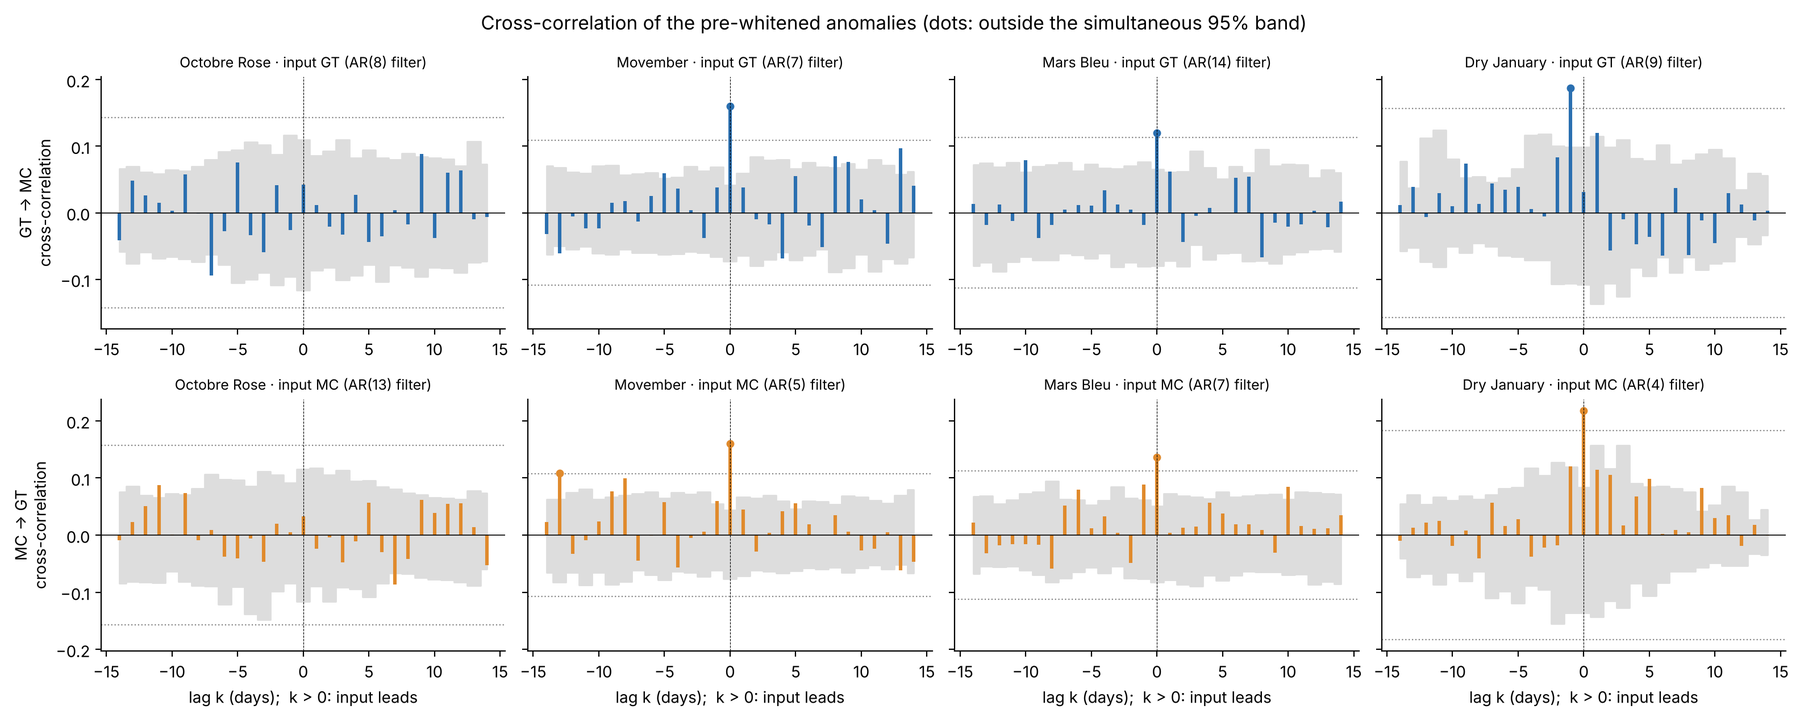
\includegraphics[width=\linewidth]{tf02_prewhitened_ccf}
  \caption{Cross-correlation of pre-whitened anomalies, GT $\to$ MC (top) and MC $\to$ GT (bottom). Positive lags: the input leads. Grey band: 95\% range over 999 season-swap surrogates; dotted lines: simultaneous 95\% band over the 29 lags. Dots mark values outside the simultaneous band.}
  \label{fig:ccf}
\end{figure}

\paragraph{Estimates.} Table~\ref{tab:tf} and Figure~\ref{fig:tfweights} give the weights. The same-day association is the dominant and most consistent feature: for Movember, Mars Bleu and Dry January, $\nu_0$ is positive has a surrogate $p$-value of 0.001 in every case but one (0.002 for Dry January GT $\to$ MC; Holm-adjusted $p=0.008$ throughout); the jackknife interval excludes zero for Movember and Mars Bleu and, narrowly, includes it for Dry January. The delay-and-decay models place the delay at 0 days in these three campaigns, with a decay $\delta$ between 0 and 0.29 (half-life under 0.6 days) in all cases but Dry January MC $\to$ GT: the associations are synchronous and brief. (The slopes of the two directions differ because the series have different spreads; the correlation is the same.) For Octobre Rose no same-day association is found, and the delay selected for a response that is not there (6 or 7 days) is unstable: the jackknife replicates give delays from 0 to 7 days (\texttt{results/tables/tf\_estimates.csv}), so it carries no information.

Lagged responses are weak. Only two of eight pairs show anything. For \textbf{Movember, GT $\to$ MC}, searches are followed by a positive lagged response (0.60, jackknife interval 0.09 to 1.10), but the test against surrogates is borderline (lagged fit: Holm-adjusted $p=0.088$; lagged sum: 0.78), and the weights are spread across lags without a clear shape (Figure~\ref{fig:tfweights}). For \textbf{Dry January, MC $\to$ GT}, coverage is followed by searches: lagged response 0.60 (0.20 to 1.01), a delay-and-decay response with gain 0.64, decay $\delta=0.77$ and half-life 2.6 days, and a 14-day cumulated response of 0.63 (0.28 to 0.97), consistent with the one-day lead of coverage in the cross-correlation. In other words, a rise of 10 points in coverage is followed by about 6 additional points of searches over two weeks. The lagged-sum test is significant after Holm correction ($p=0.024$) but the lagged-fit test is not ($p=0.41$ adjusted, 0.059 unadjusted), the sum statistic is the one that was liberal in simulation, and the window holds only 43 days per season. We treat it as a candidate to be re-examined with more seasons, not as a result.

\begin{table}[htbp]
\centering
\caption{Transfer functions on calendar-adjusted series. $\nu_0$: same-day weight; lagged: $\sum_{k=1}^{14}\nu_k$ (points of the output per point of the input), with 95\% delete-one-season jackknife intervals; $R^2_{\mathrm{lag}}$: \% of the output's unpredicted variance explained by lags 1--14 beyond the same-day term. $p$: Holm-adjusted across eight pairs, 999 season-swap surrogates (smallest attainable 0.008). $\nu_0$ is the same association in both directions.}
\label{tab:tf}
\footnotesize
\setlength{\tabcolsep}{3pt}
\resizebox{\linewidth}{!}{%
\begin{tabular}{llcccccc}
\toprule
Campaign & Direction & $\nu_0$ [95\% CI] & $p$ ($\nu_0$) & Lagged [95\% CI] & $R^2_{\mathrm{lag}}$ & $p$ (lag fit) & $p$ (lag sum) \\
\midrule
Octobre Rose & GT $\to$ MC & 0.07 [$-$0.35, 0.49] & 1.00 & 0.11 [$-$0.95, 1.16] & 2.5 & 1.00 & 1.00 \\
 & MC $\to$ GT & 0.01 [$-$0.06, 0.07] & 1.00 & 0.00 [$-$0.15, 0.15] & 3.8 & 0.87 & 1.00 \\
Movember & GT $\to$ MC & 0.51 [0.07, 0.94] & 0.008 & 0.60 [0.09, 1.10] & 4.1 & 0.088 & 0.78 \\
 & MC $\to$ GT & 0.05 [0.00, 0.10] & 0.008 & 0.01 [$-$0.10, 0.11] & 1.8 & 1.00 & 1.00 \\
Mars Bleu & GT $\to$ MC & 0.26 [0.02, 0.50] & 0.008 & $-$0.09 [$-$0.38, 0.20] & 1.9 & 1.00 & 1.00 \\
 & MC $\to$ GT & 0.06 [0.01, 0.12] & 0.008 & 0.10 [$-$0.18, 0.37] & 1.7 & 1.00 & 1.00 \\
Dry January & GT $\to$ MC & 0.18 [$-$0.02, 0.38] & 0.008 & $-$0.07 [$-$0.74, 0.61] & 3.4 & 1.00 & 1.00 \\
 & MC $\to$ GT & 0.16 [$-$0.05, 0.36] & 0.008 & 0.60 [0.20, 1.01] & 6.1 & 0.41 & 0.024 \\
\bottomrule
\end{tabular}}
\end{table}

\begin{figure}[htbp]
  \centering
  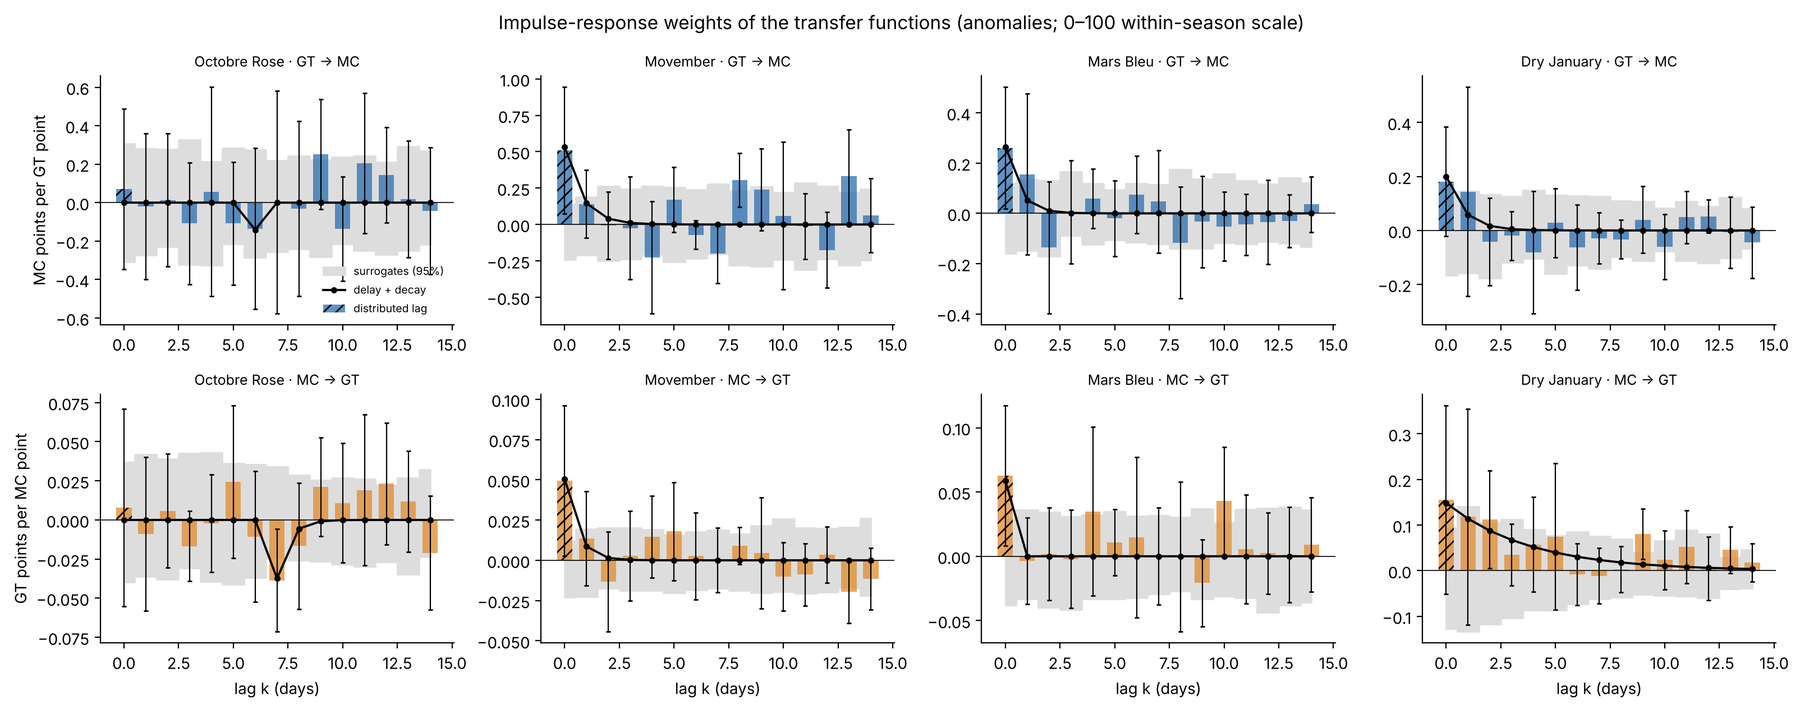
\includegraphics[width=\linewidth]{tf03_impulse_weights}
  \caption{Impulse-response weights $\nu_k$ of the transfer functions (bars: distributed lag with 95\% jackknife intervals; line: delay-and-decay model; grey band: 95\% range of each weight over season-swap surrogates; hatched bar: same-day weight). Top: GT $\to$ MC, in MC points per GT point; bottom: MC $\to$ GT.}
  \label{fig:tfweights}
\end{figure}

\paragraph{Frequency domain.} The raw series are highly coherent at low frequencies (periods above 15 days), but so are the raw series with seasons swapped, so this is the shared campaign profile (Appendix Figure~\ref{fig:coh}). In the anomalies, the squared coherence exceeds the 5\% level (0.26) at 3 of 45 frequencies for Octobre Rose, 3 of 44 for Mars Bleu, 3 of 21 for Dry January and 9 of 46 for Movember, against 1 to 2 expected by chance in each (neighbouring frequencies are correlated, so this count is indicative). Only Movember is above chance, at periods of 4 to 7 days and around 15 and 31 days; the phase delay at these frequencies ranges from $-2.7$ to $+1.7$ days with no consistent sign, which agrees with a synchronous rather than a delayed relation.

\paragraph{Summary.} Once the campaign profile and the weekly cycle are removed, searches and coverage move together \emph{on the same day} during Movember, Mars Bleu and Dry January, and not at all during Octobre Rose. Evidence of a delayed response is limited to a borderline lagged response of coverage to searches for Movember and an unconfirmed lagged response of searches to coverage for Dry January.

% ==================================================================
\section{Discussion}
% ==================================================================
\paragraph{Most of the coupling reflects the campaign calendar.} Standard Granger tests, linear or nonlinear, find links between media coverage and searches for almost every campaign. Our simulations show that a shared calendar produces exactly this pattern, and the surrogate tests remove nearly all of it on real data. The most visible campaign, Octobre Rose, is the clearest case: its media and search peaks coincide, its standard tests are highly significant, yet its day-to-day media coverage carries no information about searches beyond what any year's coverage would. In the terms of agenda-setting theory \cite{mccombs1972}, our results do not support a strong, day-to-day transfer of attention from the media to the public during these campaigns; both channels respond to the same calendar.

\paragraph{Movember.} The only link that resists the weekly cycle and the season levels is Movember, MC $\to$ GT, detected by lsNGC. It is small, and three observations limit its reading. It disappears when the average campaign profile is subtracted from both series; the transfer function of the adjusted series has no lagged response of searches to coverage (0.01, interval $-0.10$ to $0.11$); and the linear impulse response of the raw series is negative, in line with the media peak coming about nine days after the search peak (Table~\ref{tab:peaklag}). Together these suggest that coverage carries information about searches through the shape of the campaign in each year, not through day-to-day departures from it. Whether this shape is the size of the campaign, its timing, or an interaction between the two we cannot tell; describing it (for instance with partial-dependence plots of the lsNGC model, or by relating season-level features of the two series) is the next step. With 11 seasons, the precision is limited: the 95\% intervals of the lagged response of searches to coverage (Table~\ref{tab:tf}) are about $\pm0.15$ search points per coverage point for Movember and Octobre Rose and $-0.18$ to $0.37$ for Mars Bleu, so larger lagged responses are excluded in those campaigns, but not in Dry January.

\paragraph{Same-day association.} The transfer functions show a positive association on the same day for Movember, Mars Bleu and Dry January after the campaign profile, the weekly cycle and the season levels are removed, and none for Octobre Rose. A same-day correlation has no direction, and daily data cannot order two events within a day. It is what a shared event (a news item, a public figure's announcement) produces, and also what a fast mutual reaction produces. The simulations add a caution: when the timing of the campaign pulse varies from year to year, the same-day test rejects in about half the datasets without any link. Resolving the order would need data at a finer resolution (hourly Google Trends, time-stamped articles) or events whose timing is known to be unrelated to the campaign.

\paragraph{Predictive, not causal.} A surrogate test removes a common driver with the same timing every year, but not one whose date changes from year to year, such as news events, celebrity announcements or local initiatives; the simulations show that no test used here, transfer functions included, can rule this out. The Movember and same-day results are therefore predictive associations beyond a fixed campaign calendar, not evidence of a causal effect of media coverage.

\paragraph{Limitations.} Besides the data-quality issues of Section~\ref{sec:data} (sampling noise of GT, normalisation within seasons, scope of the MC collection): (i) the KPSS test indicates a non-constant mean for four of the eight series; the within-season design and the surrogates limit, but do not remove, the influence of trends across seasons, in particular for Dry January. (ii) Queries rely on manual curation; the Dry January GT query includes general alcohol-cessation terms, and MC texts contain boilerplate (cookie banners, newsletter links; Figure~\ref{fig:kgrams}) that may add noise to the k-gram selection. (iii) Many specifications were run: three methods, two calendar-conditioning variants and five calendar adjustments for the surrogate tests, and 24 transfer-function tests. Multiple-testing corrections are applied within each family of eight tests, not across families, so a single significant cell is weak evidence. The Movember lsNGC result is the only one that repeats across variants, but its unadjusted $p$-value of 0.001, the smallest attainable with 999 surrogates, would reach 0.048 after a Bonferroni correction over the 48 tests of the main analysis; we report all specifications and base conclusions on links that are consistent across them. (iv) The nonlinear analysis truncates seasons to the shortest season of each campaign and uses lag orders up to 7 days, whereas the linear analysis selects lags up to 20 days, so effect sizes are not directly comparable between the two. (v) The surrogate and transfer-function tests are calibrated on simulated systems whose structure we chose; the simulated weekly cycle did not reproduce the influence that the real weekly cycle has on the linear and KGC tests. (vi) Each seasonal window of GT was downloaded once, and the transfer functions of Dry January rest on 43 days per season.

\paragraph{Scope.} The analysis describes how media coverage and search interest co-evolve during campaigns. It does not estimate the counterfactual trajectory in the absence of a campaign, nor does it measure downstream outcomes such as screening uptake.

% ==================================================================
\section{Conclusion and future work}
% ==================================================================
Through query construction, peak-alignment analysis, linear and nonlinear Granger tests with calendar-adjusted surrogates, and transfer functions, all checked on simulated systems where the true answer is known, we find that most of the apparent coupling between media coverage and public interest during French health campaigns reflects their shared calendar. What remains is, first, a same-day association between searches and coverage for Movember, Mars Bleu and Dry January, whose direction the daily data cannot establish; second, one small nonlinear link from coverage to searches for Movember, stable to the weekly cycle and to season levels but dependent on the campaign profile, so not a day-to-day response; and third, nothing for Octobre Rose, the campaign with the strongest standard tests. A delayed response of one series to the other, the quantity a transfer function adds to a Granger test, is established for no campaign.

Future work will (i) use media shocks unrelated to the campaign calendar, such as news events or celebrity announcements, to identify the effect of coverage on searches; (ii) use hourly search data and time-stamped articles to order the same-day association; (iii) relate the Movember link to season-level features (size and timing of the campaign) to characterise what it carries; (iv) estimate campaign effects with an event-study design against control topics without a campaign; and (v) link search interest to downstream outcomes such as screening uptake.

% ==================================================================
\begin{thebibliography}{99}
\bibitem{akaike1974} H.~Akaike. A new look at the statistical model identification. \emph{IEEE Transactions on Automatic Control}, 19(6):716--723, 1974.
\bibitem{ayers2016} J.~W. Ayers, J.~L. Westmaas, E.~C. Leas, A.~Benton, Y.~Chen, M.~Dredze and B.~M. Althouse. Leveraging big data to improve health awareness campaigns: a novel evaluation of the Great American Smokeout. \emph{JMIR Public Health and Surveillance}, 2(1):e16, 2016.
\bibitem{box2015} G.~E.~P. Box, G.~M. Jenkins, G.~C. Reinsel and G.~M. Ljung. \emph{Time Series Analysis: Forecasting and Control}, 5th edition. Wiley, 2015.
\bibitem{dickey1979} D.~A. Dickey and W.~A. Fuller. Distribution of the estimators for autoregressive time series with a unit root. \emph{Journal of the American Statistical Association}, 74(366):427--431, 1979.
\bibitem{eysenbach2009} G.~Eysenbach. Infodemiology and infoveillance: framework for an emerging set of public health informatics methods to analyze search, communication and publication behavior on the Internet. \emph{Journal of Medical Internet Research}, 11(1):e11, 2009.
\bibitem{glynn2011} R.~W. Glynn, J.~C. Kelly, N.~Coffey, K.~J. Sweeney and M.~J. Kerin. The effect of breast cancer awareness month on internet search activity -- a comparison with awareness campaigns for lung and prostate cancer. \emph{BMC Cancer}, 11:442, 2011.
\bibitem{gonzalezpadilla2021} D.~A. Gonz\'alez-Padilla, R.~Espa\~na-Navarro, J.~D. Subiela, R.~Kumar, L.~G. Medina, J.~Aumatell, J.~M. De la Morena-Gallego and G.~E. Cacciamani. Is ``Movember'' an effective prostate cancer awareness campaign beyond the English language? Insights from Google Trends among Spanish speakers. \emph{Soci\'et\'e Internationale d'Urologie Journal}, 2(6):362--369, 2021.
\bibitem{granger1969} C.~W.~J. Granger. Investigating causal relations by econometric models and cross-spectral methods. \emph{Econometrica}, 37(3):424--438, 1969.
\bibitem{holm1979} S.~Holm. A simple sequentially rejective multiple test procedure. \emph{Scandinavian Journal of Statistics}, 6(2):65--70, 1979.
\bibitem{kwak2018} H.~Kwak, J.~An, J.~Salminen, S.-G. Jung and B.~J. Jansen. What we read, what we search: media attention and public attention among 193 countries. In \emph{Proceedings of The Web Conference (WWW)}, 2018.
\bibitem{kwiatkowski1992} D.~Kwiatkowski, P.~C.~B. Phillips, P.~Schmidt and Y.~Shin. Testing the null hypothesis of stationarity against the alternative of a unit root. \emph{Journal of Econometrics}, 54(1--3):159--178, 1992.
\bibitem{marinazzo2008} D.~Marinazzo, M.~Pellicoro and S.~Stramaglia. Kernel method for nonlinear Granger causality. \emph{Physical Review Letters}, 100(14):144103, 2008.
\bibitem{mccombs1972} M.~E. McCombs and D.~L. Shaw. The agenda-setting function of mass media. \emph{Public Opinion Quarterly}, 36(2):176--187, 1972.
\bibitem{murphy2026} F.~Murphy and A.~Benavoli. Constraint- and score-based nonlinear Granger causality discovery with kernels. arXiv:2601.09579 (preprint), 2026.
\bibitem{mavragani2019} A.~Mavragani and G.~Ochoa. Google Trends in infodemiology and infoveillance: methodology framework. \emph{JMIR Public Health and Surveillance}, 5(2):e13439, 2019.
\bibitem{nuti2014} S.~V. Nuti et al. The use of Google Trends in health care research: a systematic review. \emph{PLoS ONE}, 9(10):e109583, 2014.
\bibitem{roberts2021} H.~Roberts et al. Media Cloud: Massive open source collection of global news on the open web. In \emph{Proceedings of ICWSM}, 2021.
\bibitem{theiler1992} J.~Theiler, S.~Eubank, A.~Longtin, B.~Galdrikian and J.~D. Farmer. Testing for nonlinearity in time series: the method of surrogate data. \emph{Physica D}, 58(1--4):77--94, 1992.
\bibitem{weeks2010} B.~Weeks and B.~Southwell. The symbiosis of news coverage and aggregate online search behavior: Obama, rumors, and presidential politics. \emph{Mass Communication and Society}, 13(4):341--360, 2010.
\bibitem{wismuller2021} A.~Wismüller, A.~M. Dsouza, M.~A. Vosoughi and A.~Abidin. Large-scale nonlinear Granger causality for inferring directed dependence from short multivariate time-series data. \emph{Scientific Reports}, 11:7817, 2021.
\end{thebibliography}

% ==================================================================
\appendix
\section{Query construction}\label{app:queries}
\begin{table}[H]
\centering
\caption{Queries used for the daily series. Google Trends queries are those stored in the daily data files. The MediaCloud files do not record their query; the terms below are the k-gram selection.}
\small
\begin{tabularx}{\linewidth}{lXX}
\toprule
Campaign & Google Trends (terms combined with +) & MediaCloud (terms combined with OR) \\
\midrule
Octobre Rose & Octobre rose, cancer du sein, mammographie, dépistage cancer du sein, cancer du sein symptôme & octobre rose, cancer sein, lutte contre cancer sein, dépistage cancer sein, mois octobre rose \\
Dry January & dry january, mois sans alcool, arreter de boire, janvier sans alcool, arreter alcool & dry january, consommation alcool, mois alcool, boire alcool mois, dry january janvier, alcool mois janvier \\
Movember & Movember, cancer prostate, movember prostate, cancer prostate psa, cancer prostate traitement & movember, cancer prostate, mois movember, masculin cancer prostate, maladie masculin cancer prostate \\
Mars Bleu & Mars bleu, cancer colorectal, dépistage colon, coloscopie, cancer colon & mars bleu, cancer colorectal, dépistage cancer colorectal, cancer colorectal cancer, mois mars bleu \\
\bottomrule
\end{tabularx}
\end{table}

\begin{figure}[htbp]
  \centering
  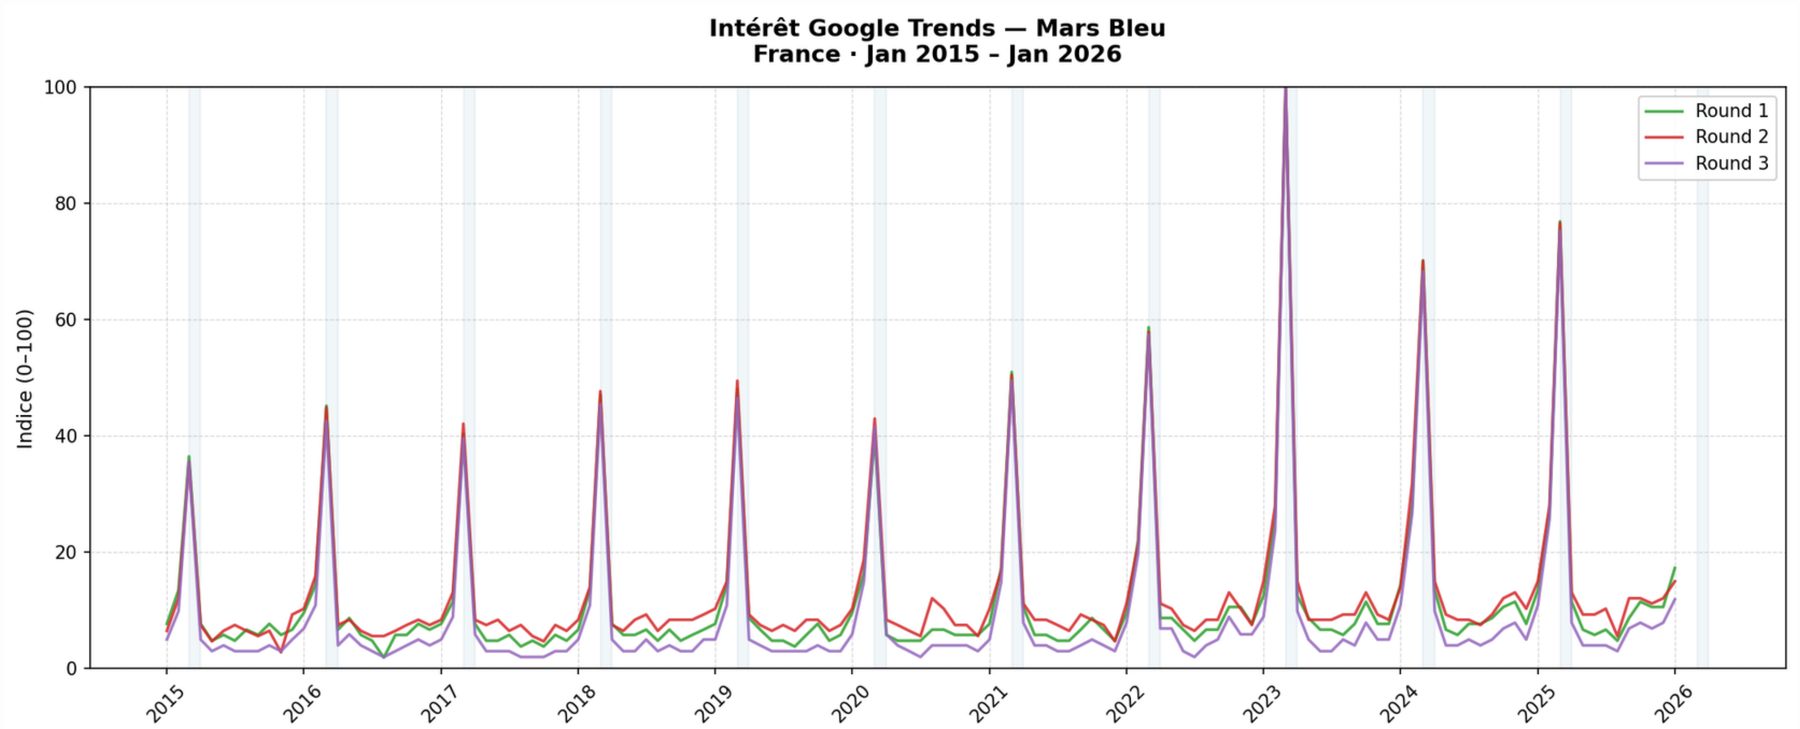
\includegraphics[width=\linewidth]{figure15b}
  \caption{Google Trends signal for Mars Bleu after three snowball-sampling rounds: the shape is stable across rounds.}
  \label{fig:snowball}
\end{figure}

\begin{figure}[htbp]
  \centering
  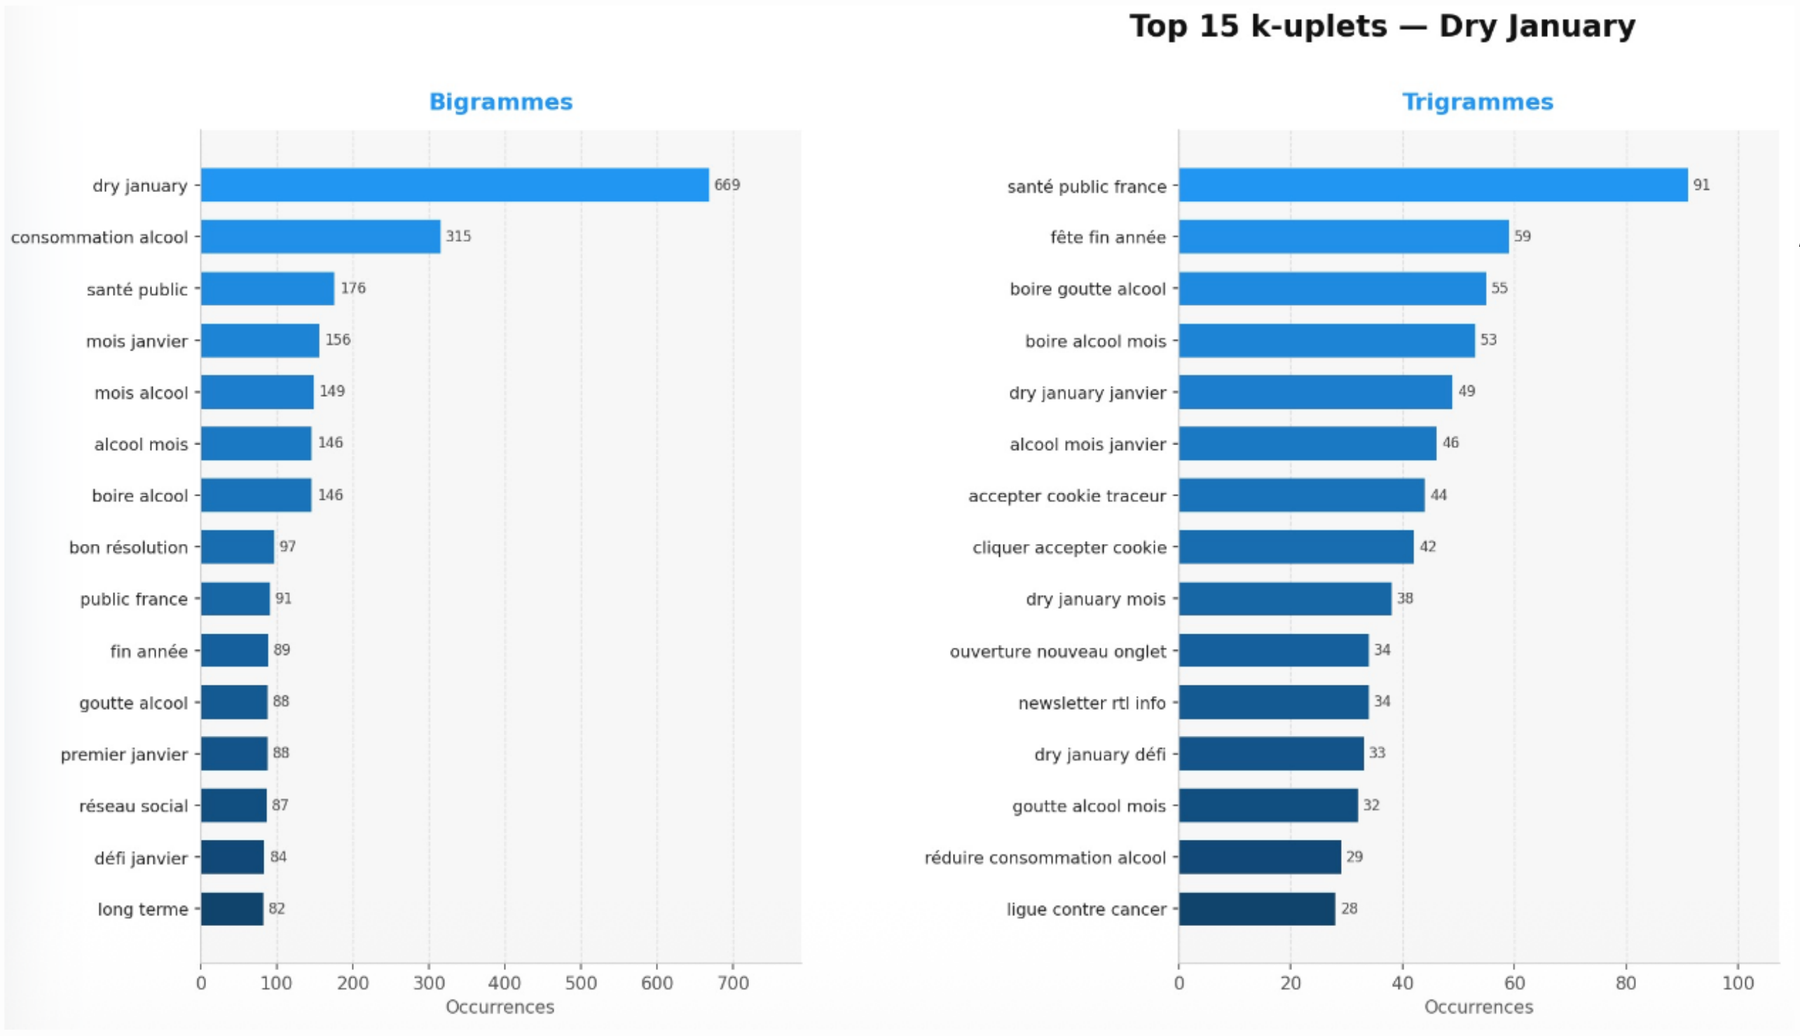
\includegraphics[width=\linewidth]{figure16}
  \caption{Top-15 bigrams and trigrams in MediaCloud articles retrieved for Dry January, used as the basis for the MC query.}
  \label{fig:kgrams}
\end{figure}

\section{Stationarity tests}\label{app:stationarity}
\begin{table}[H]
\centering
\caption{ADF (null: unit root) and KPSS (null: stationarity) tests on the concatenated daily series. KPSS p-values are bounded to $[0.01, 0.10]$ by the look-up table: 0.01 means $\le 0.01$ and 0.10 means $\ge 0.10$.}
\small
\begin{tabular}{llcccc}
\toprule
Campaign & Series & ADF statistic & ADF p-value & KPSS statistic & KPSS p-value \\
\midrule
Dry January  & GT & $-6.51$ & $1.1\times10^{-8}$  & 0.859 & 0.01 \\
             & MC & $-6.70$ & $4.0\times10^{-9}$  & 0.756 & 0.01 \\
Mars Bleu    & GT & $-4.70$ & $8.4\times10^{-5}$  & 0.120 & 0.10 \\
             & MC & $-6.70$ & $4.0\times10^{-9}$  & 0.671 & 0.016 \\
Movember     & GT & $-6.32$ & $3.1\times10^{-8}$  & 0.117 & 0.10 \\
             & MC & $-8.44$ & $1.8\times10^{-13}$ & 0.077 & 0.10 \\
Octobre Rose & GT & $-5.31$ & $5.1\times10^{-6}$  & 1.063 & 0.01 \\
             & MC & $-6.07$ & $1.1\times10^{-7}$  & 0.158 & 0.10 \\
\bottomrule
\end{tabular}
\end{table}

\section{Sensitivity of the linear tests to the specification}\label{app:sensitivity}
\begin{table}[H]
\centering
\caption{Linear Granger causality under three specifications: lags across season boundaries with AIC computed on a different sample for each lag pair (original specification); the same with AIC on a common sample; and AIC on a common sample with within-season lags (main specification, Table~\ref{tab:granger}). Unadjusted p-values; LOYO: folds with $p<0.05$.}
\footnotesize
\setlength{\tabcolsep}{3pt}
\resizebox{\linewidth}{!}{%
\begin{tabular}{llcccccc}
\toprule
 & & \multicolumn{2}{c}{Original} & \multicolumn{2}{c}{Common-sample AIC} & \multicolumn{2}{c}{Within-season lags} \\
\cmidrule(lr){3-4}\cmidrule(lr){5-6}\cmidrule(lr){7-8}
Campaign & Direction & $(p^*,q^*)$, p & LOYO & $(p^*,q^*)$, p & LOYO & $(p^*,q^*)$, p & LOYO \\
\midrule
Dry January  & GT $\to$ MC & (7,20), $8.9\times10^{-4}$   & 11/11 & (7,1), $4.4\times10^{-11}$  & 11/11 & (18,1), 0.27 & 0/11 \\
             & MC $\to$ GT & (20,1), $1.5\times10^{-4}$   & 10/11 & (3,1), $4.0\times10^{-4}$   & 11/11 & (9,1), $2.6\times10^{-5}$ & 10/11 \\
Mars Bleu    & GT $\to$ MC & (7,20), $2.7\times10^{-5}$   & 11/11 & (7,16), $3.7\times10^{-6}$  & 11/11 & (10,16), $1.2\times10^{-8}$ & 11/11 \\
             & MC $\to$ GT & (20,1), 0.027                & 10/11 & (19,1), 0.027               & 10/11 & (17,1), 0.42 & 0/11 \\
Movember     & GT $\to$ MC & (7,20), $3.6\times10^{-8}$   & 11/11 & (7,16), $1.7\times10^{-8}$  & 11/11 & (1,16), $3.7\times10^{-11}$ & 11/11 \\
             & MC $\to$ GT & (20,2), $2.2\times10^{-3}$   & 11/11 & (8,2), $2.6\times10^{-3}$   & 11/11 & (8,2), $5.0\times10^{-3}$ & 11/11 \\
Octobre Rose & GT $\to$ MC & (13,20), $4.9\times10^{-11}$ & 11/11 & (13,15), $6.4\times10^{-12}$ & 11/11 & (13,15), $8.5\times10^{-10}$ & 11/11 \\
             & MC $\to$ GT & (20,7), $7.2\times10^{-4}$   & 11/11 & (8,7), $4.0\times10^{-4}$   & 11/11 & (8,7), $7.4\times10^{-4}$ & 11/11 \\
\bottomrule
\end{tabular}}
\end{table}

With AIC computed on a different sample for each lag pair, one of the two lag orders reaches the upper bound of the grid in all eight models; with a common sample, no selected order reaches it.

\paragraph{Season fixed effects.} Seasons differ in the level of each series, and the models above have a single intercept; the past of the cause could then predict the effect only because both series are high in the same seasons. Adding one intercept per season to both models, with the lag orders and observations of Table~\ref{tab:granger}, leaves the conclusions unchanged: the Holm-adjusted $p$-values are below $10^{-7}$ for the GT $\to$ MC tests of Mars Bleu, Movember and Octobre Rose, $1.4\times10^{-4}$ (Dry January), 0.014 (Movember) and 0.027 (Octobre Rose) for MC $\to$ GT, and 0.29 for Dry January GT $\to$ MC and Mars Bleu MC $\to$ GT (\texttt{results/tables/season\_fixed\_effects.csv}).

\section{Linear Granger causality: lag selection and coefficients}\label{app:linfigs}
\begin{figure}[htbp]
  \centering
  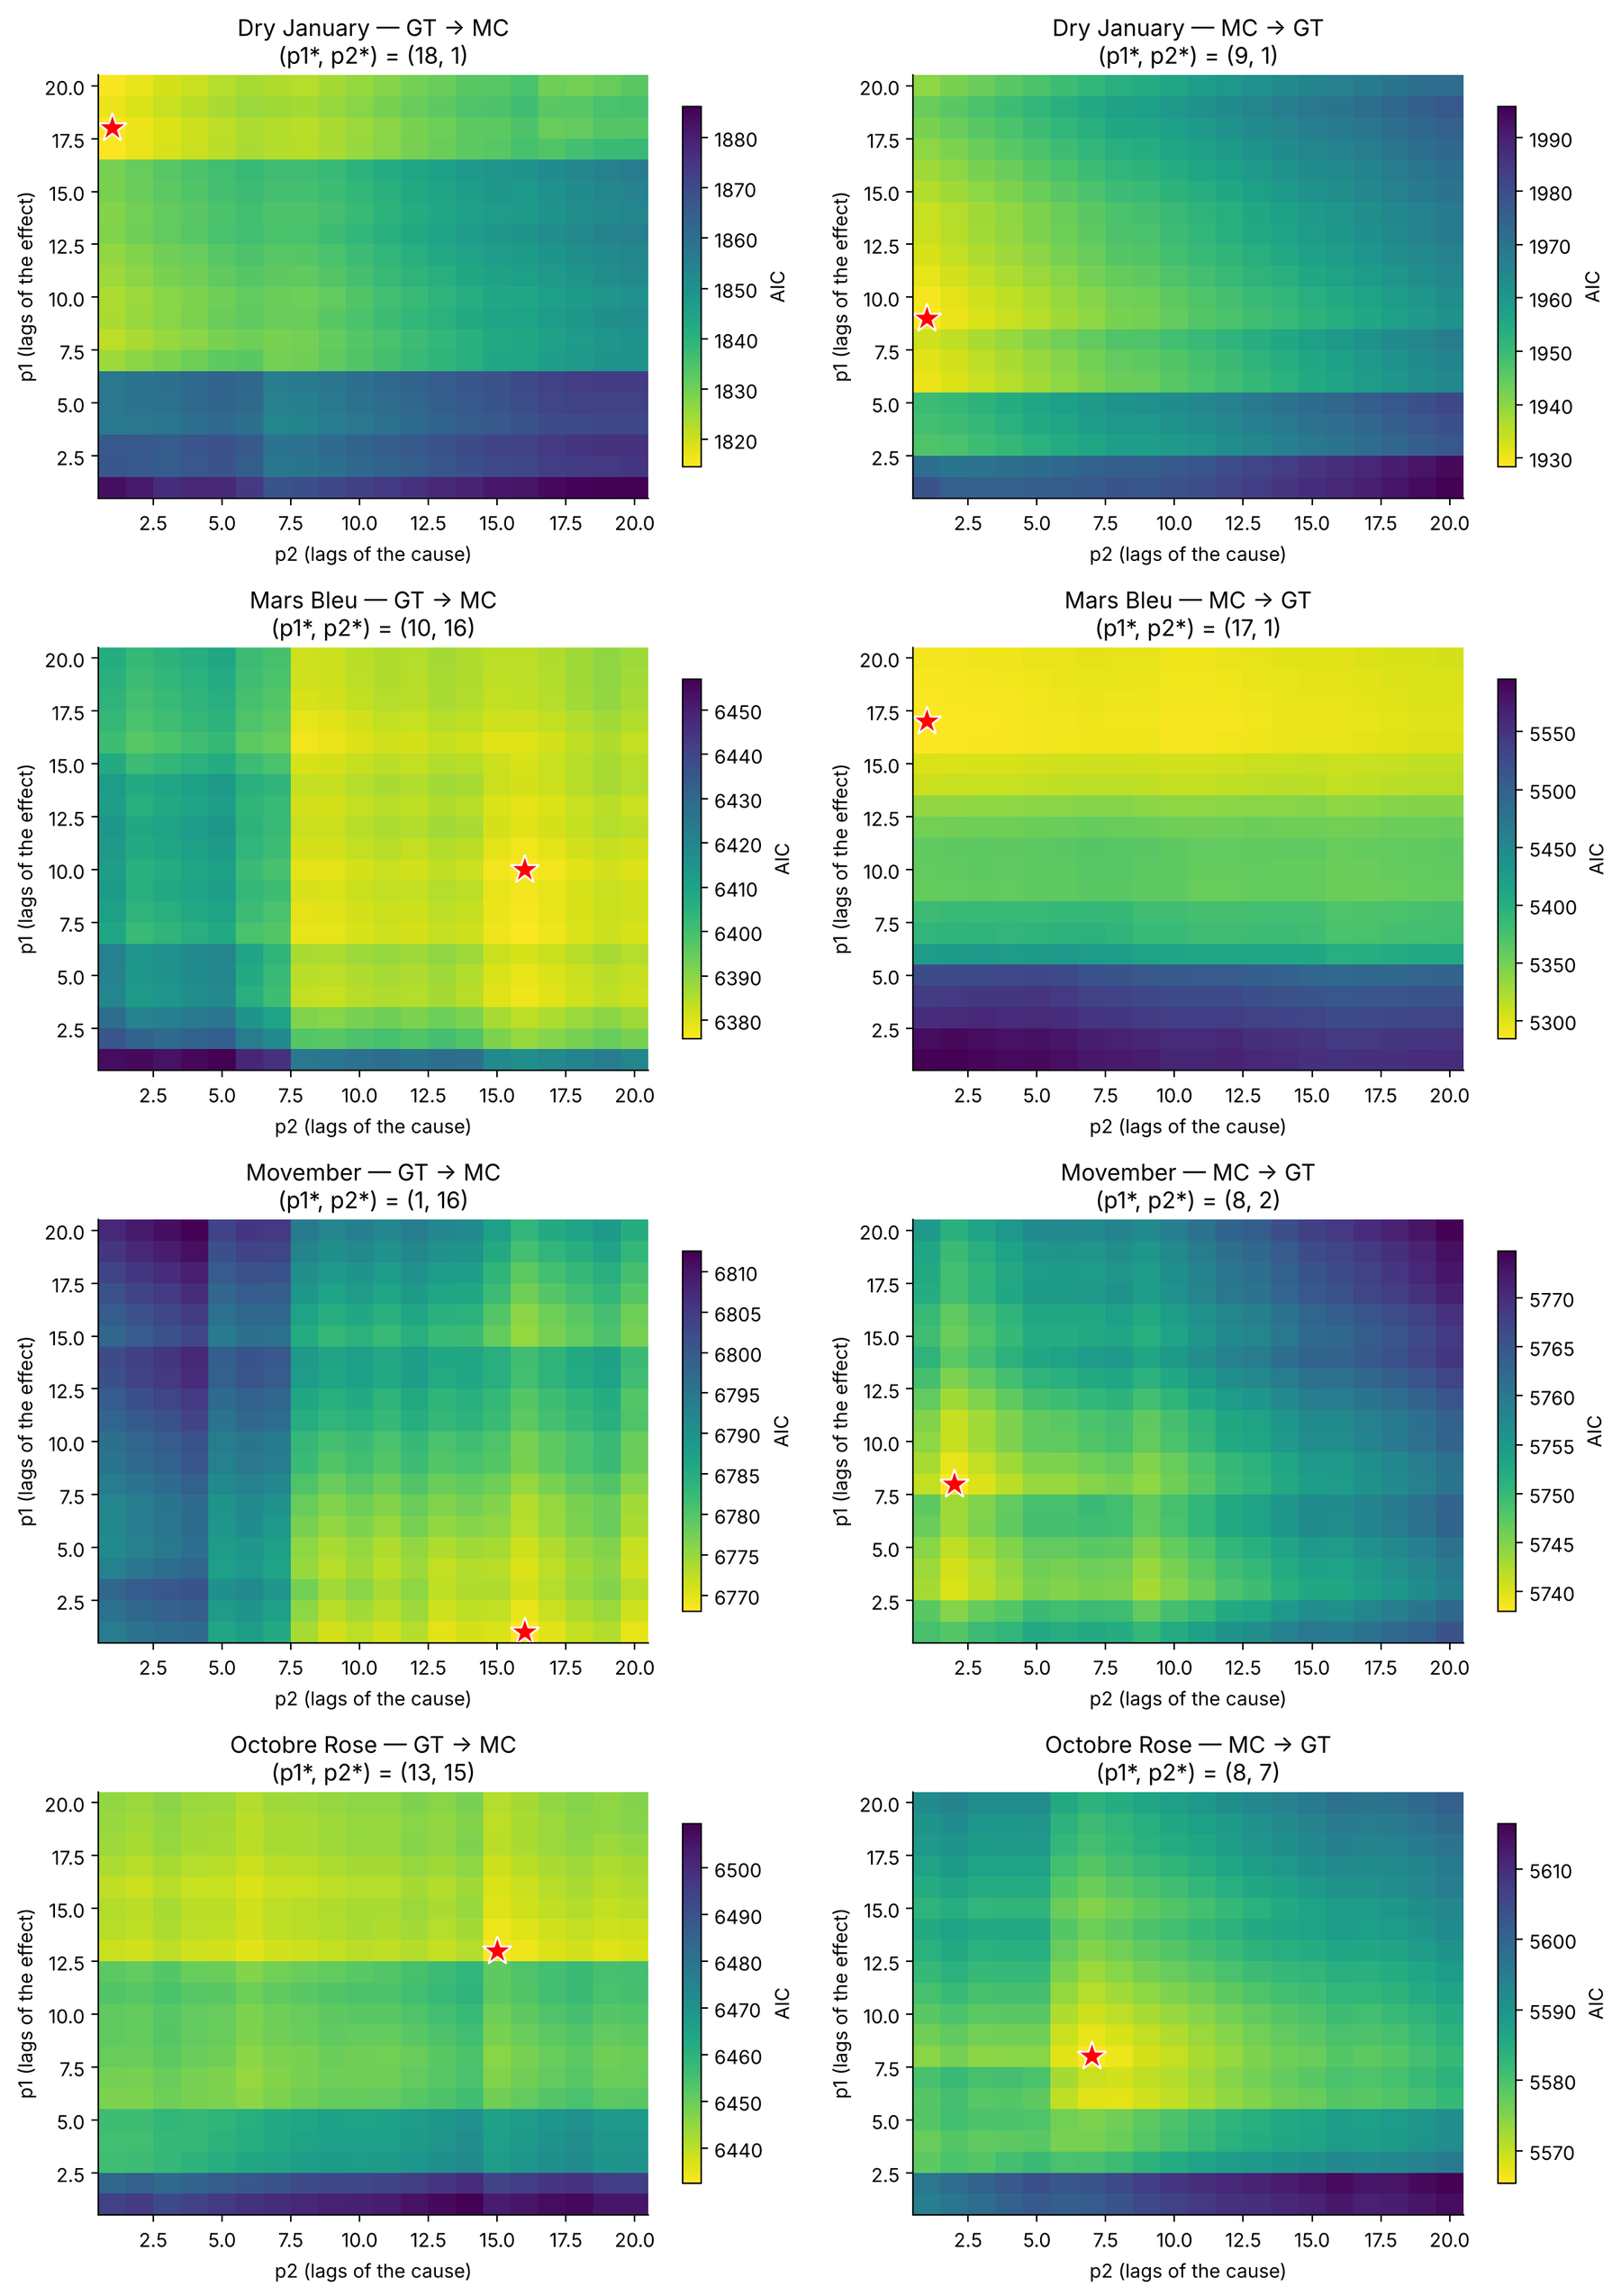
\includegraphics[width=\linewidth]{fig11_aic_all_campaigns}
  \caption{AIC of the full model as a function of the lag orders for all campaigns (rows) and both directions (left: GT $\to$ MC; right: MC $\to$ GT), with within-season lags and a common sample. The star marks the AIC minimum.}
  \label{fig:aic-all}
\end{figure}

\begin{figure}[htbp]
  \centering
  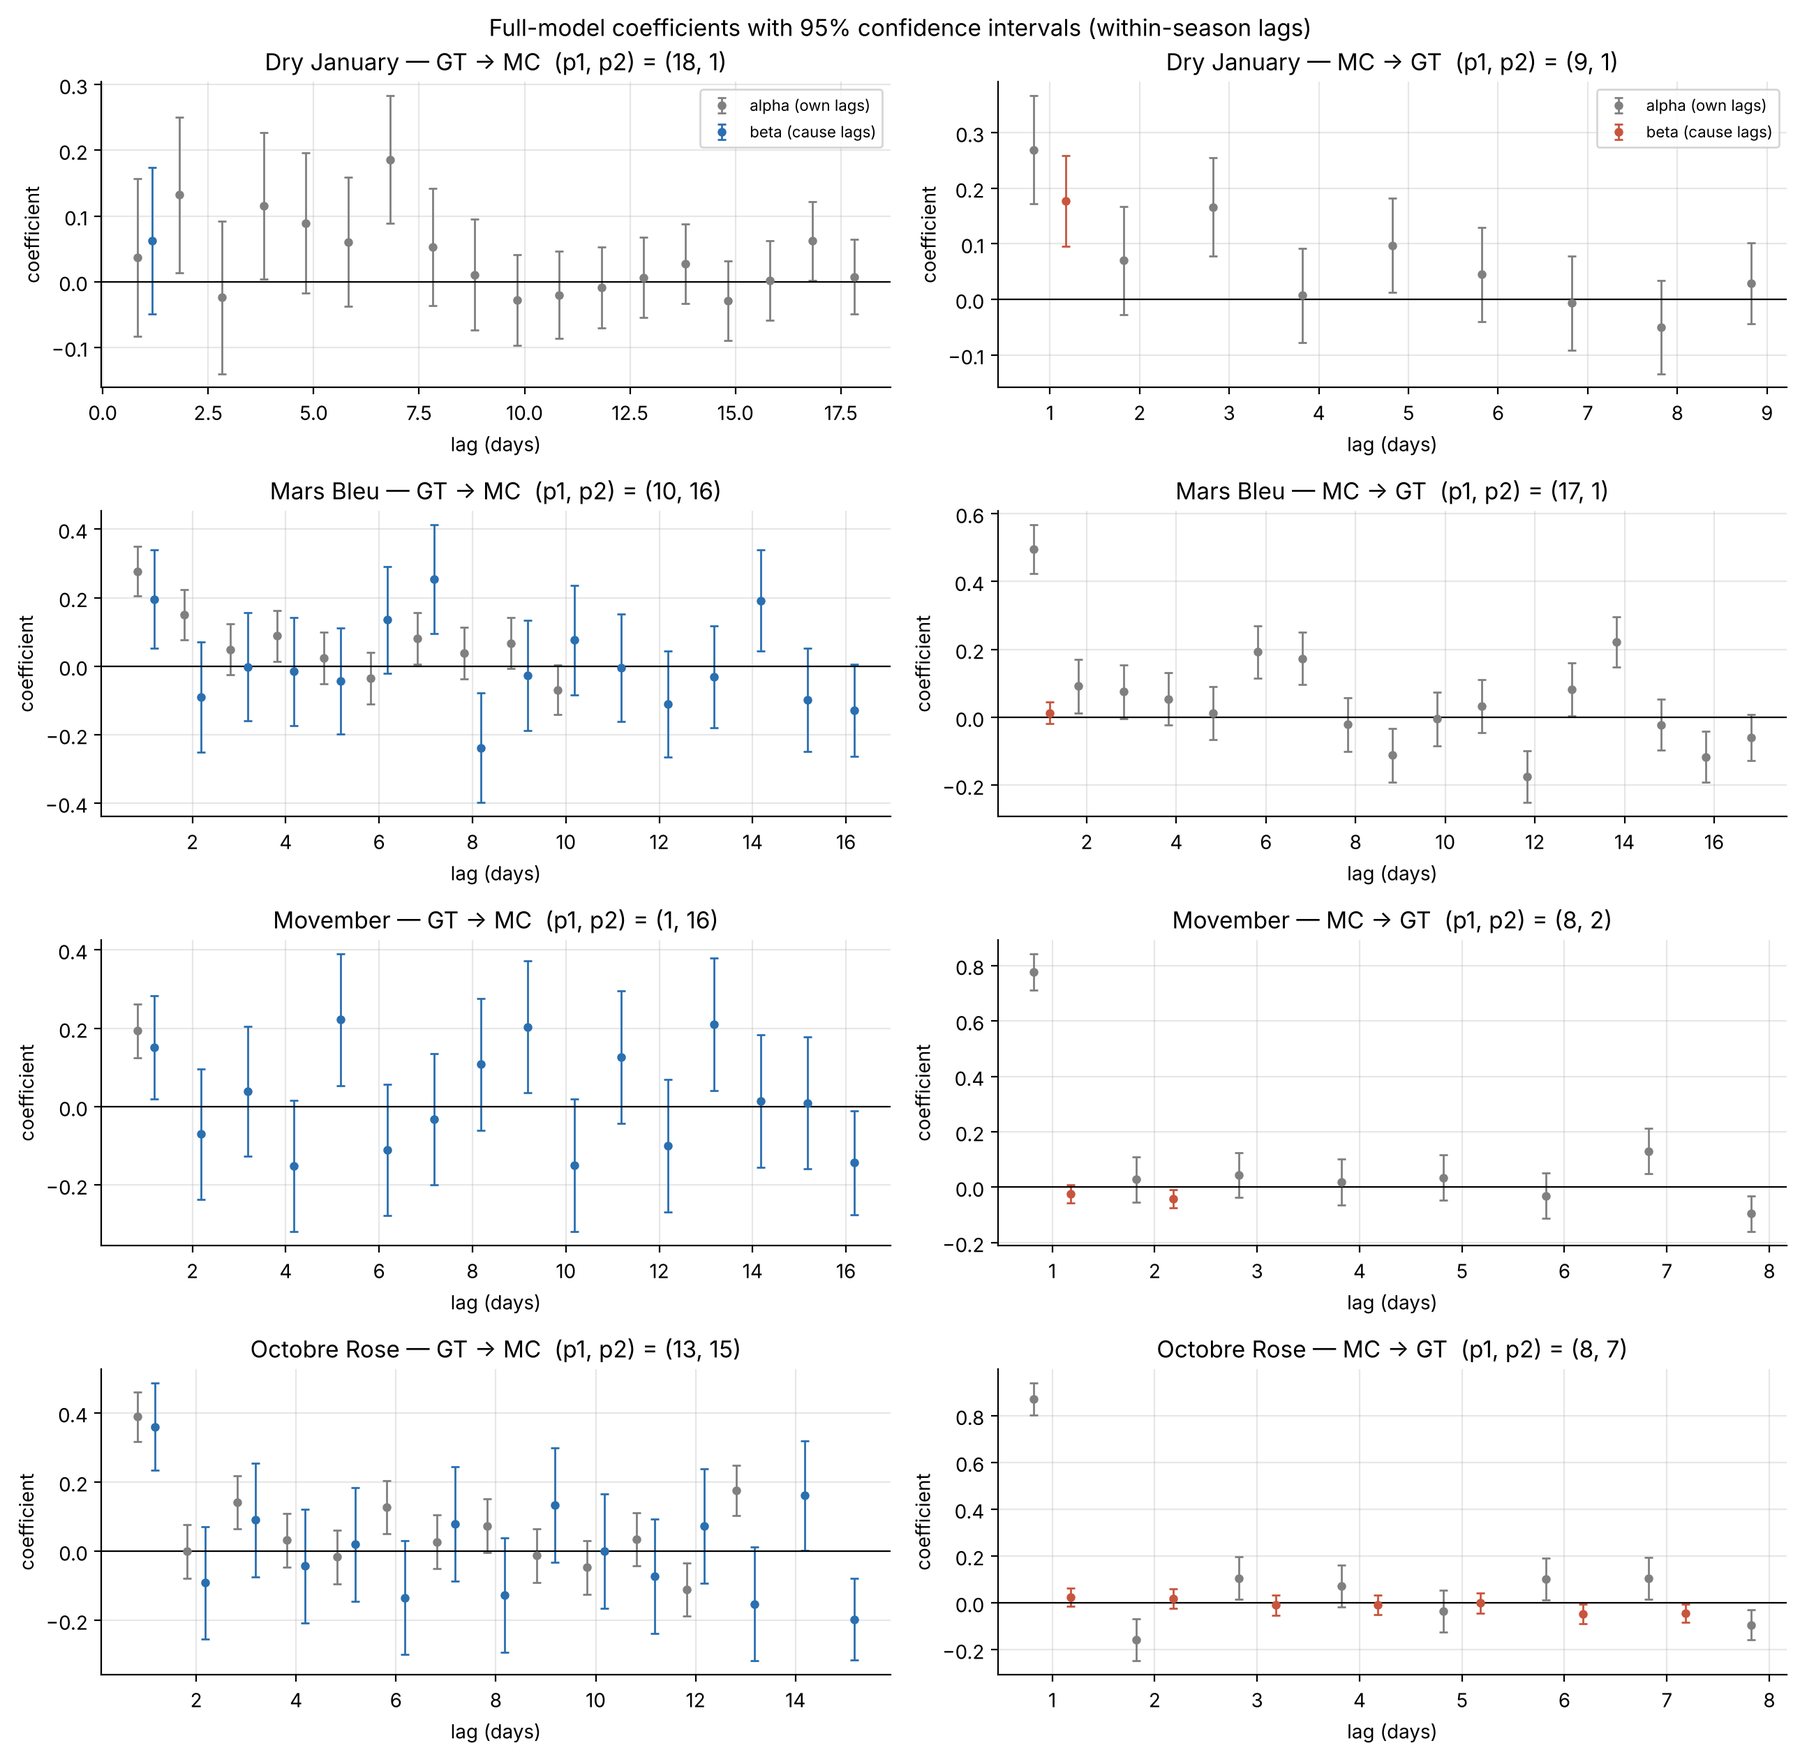
\includegraphics[width=\linewidth]{fig12_coefficients}
  \caption{Estimated autoregressive ($\alpha_k$, grey) and cross-lag ($\beta_k$, coloured) coefficients of the full models by lag, with 95\% confidence intervals, for each campaign and direction (within-season lags).}
  \label{fig:coefs}
\end{figure}

\section{Transfer functions: supplementary figures}\label{app:tf}
\begin{figure}[htbp]
  \centering
  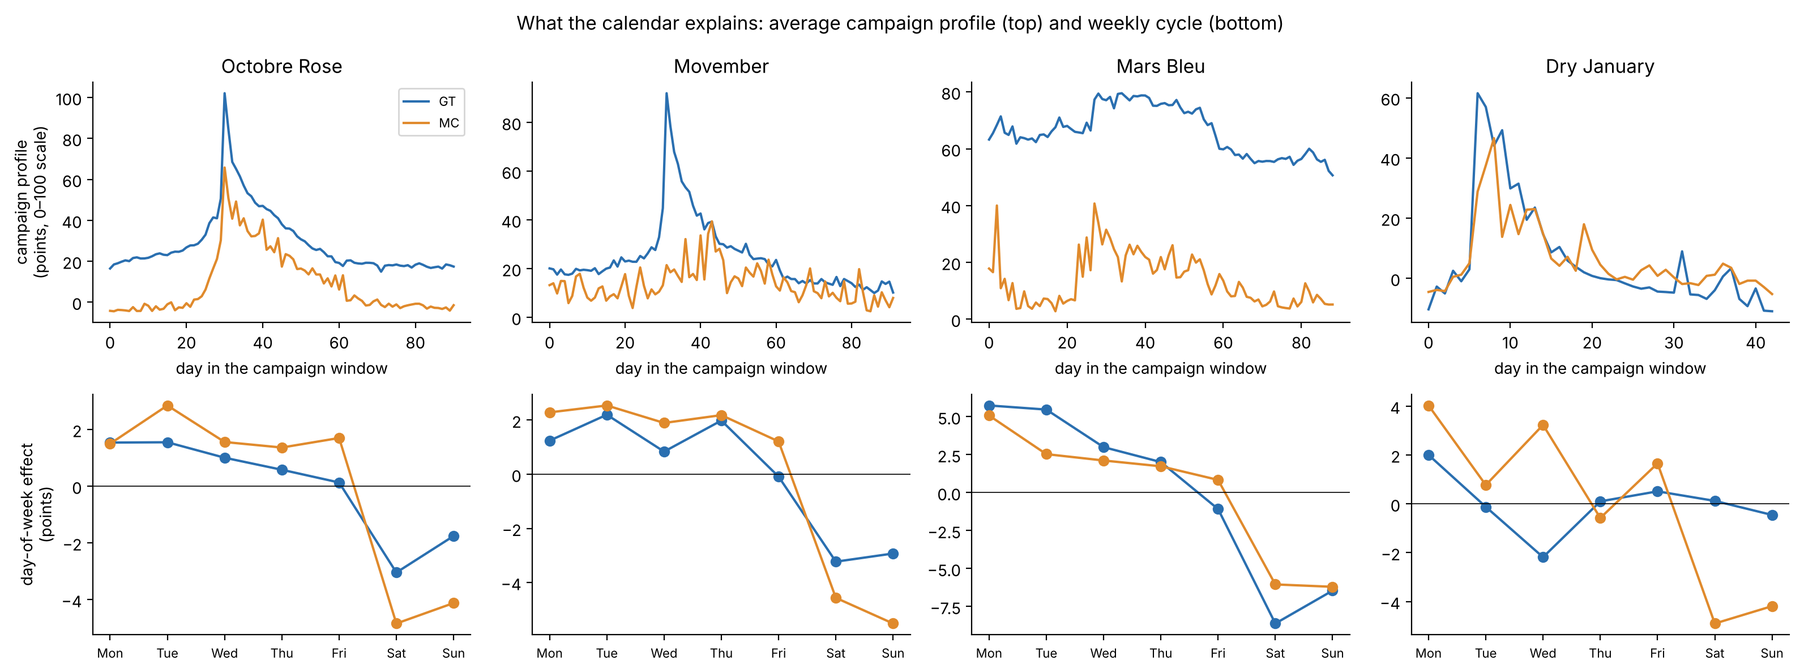
\includegraphics[width=\linewidth]{tf01_calendar_components}
  \caption{Calendar components removed before estimating transfer functions: average campaign profile (top) and day-of-week effect (bottom), in points of the 0--100 within-season scale.}
  \label{fig:tfcal}
\end{figure}

\begin{figure}[htbp]
  \centering
  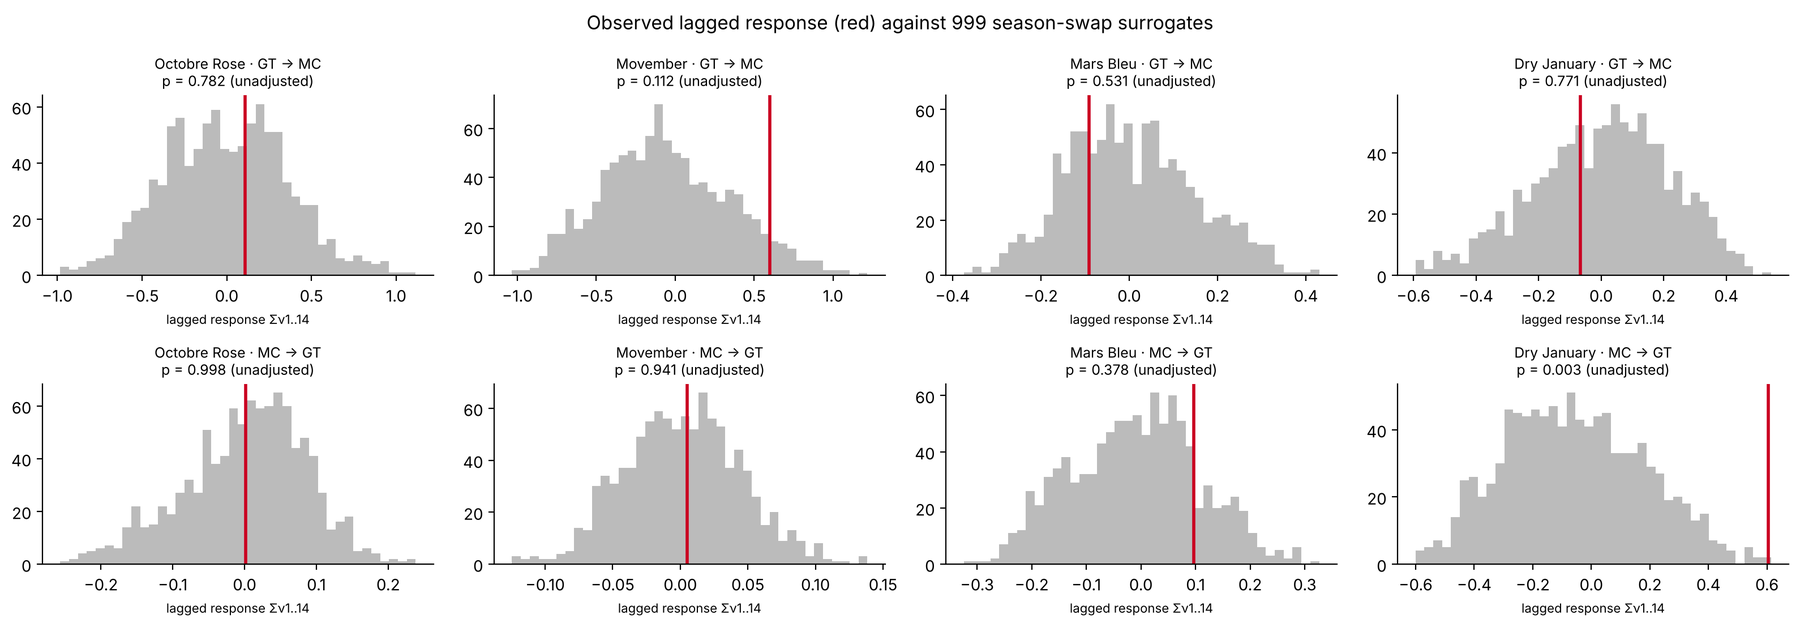
\includegraphics[width=\linewidth]{tf04_lagged_response_null}
  \caption{Lagged response $\sum_{k=1}^{14}\nu_k$ (red line) against its distribution over 999 season-swap surrogates, unadjusted two-sided $p$-values.}
  \label{fig:tfnull}
\end{figure}

\begin{figure}[htbp]
  \centering
  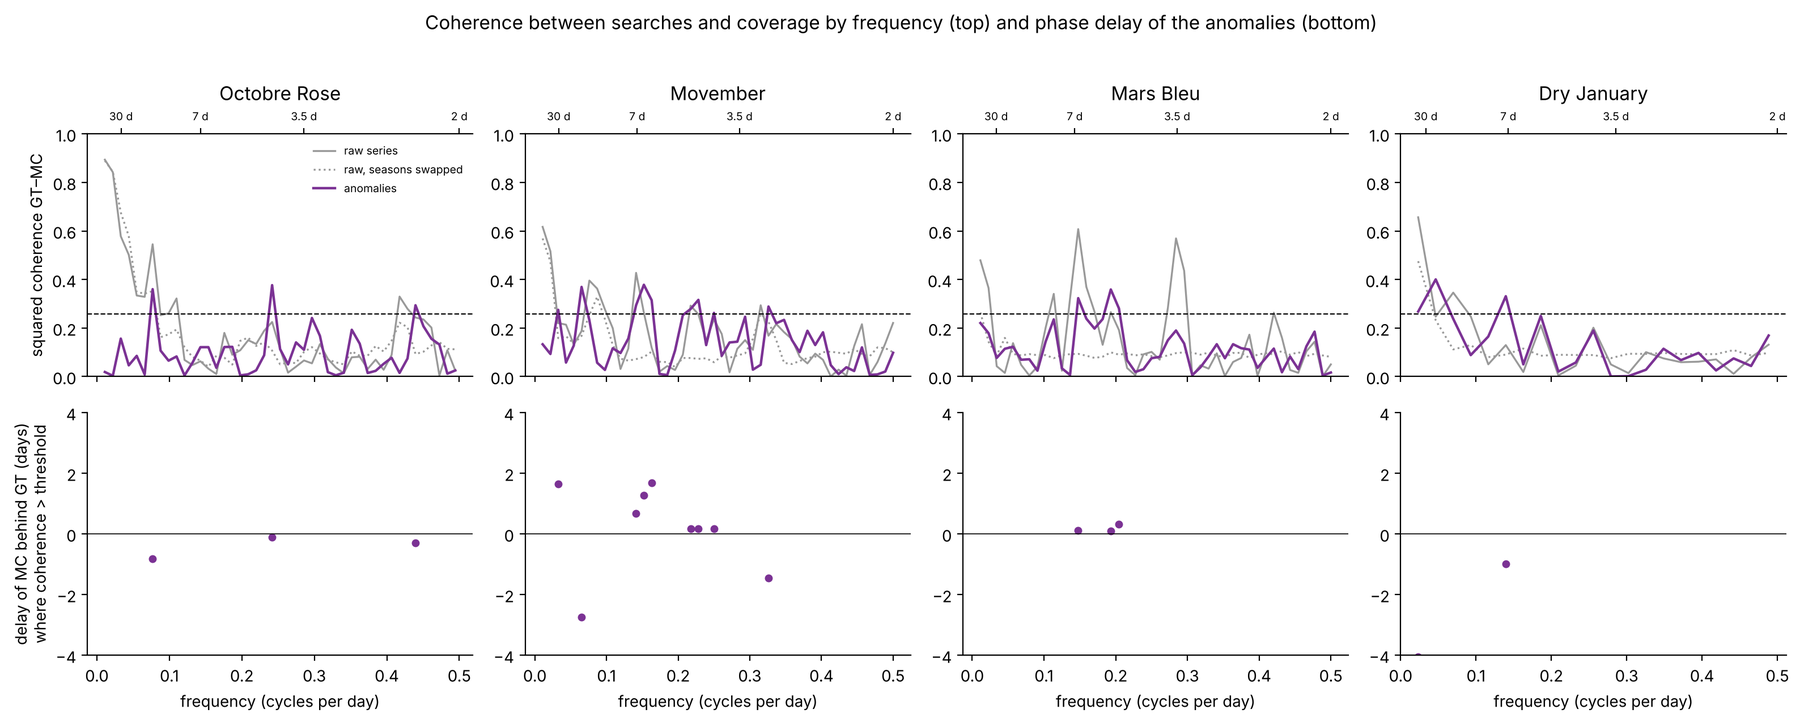
\includegraphics[width=\linewidth]{tf05_coherence}
  \caption{Squared coherence between GT and MC by frequency (top) for the raw series, the raw series with seasons swapped (mean over 200 swaps: what the calendar alone produces) and the anomalies; dashed line: level exceeded by 5\% of unrelated series with 11 seasons. Bottom: delay of MC behind GT where the coherence of the anomalies exceeds this level.}
  \label{fig:coh}
\end{figure}

\section{Calendar adjustments of the nonlinear tests}\label{app:adjust}
\begin{figure}[htbp]
  \centering
  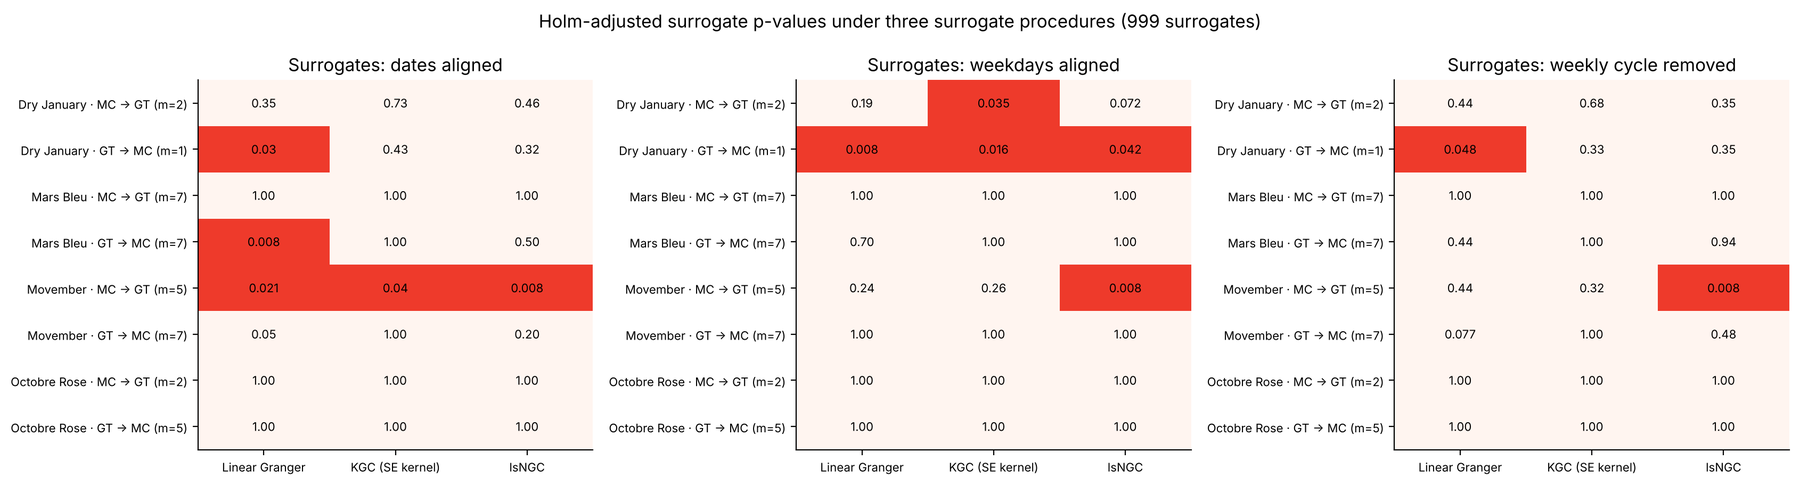
\includegraphics[width=\linewidth]{kg08_weekly_cycle}
  \caption{Holm-adjusted surrogate $p$-values (999 surrogates) of linear Granger causality, KGC and lsNGC when the surrogate cause is another season aligned by calendar date (left; adjustment A), another season shifted by at most three days so that weekdays coincide (centre), or when the weekly cycle is first removed from both series (right; adjustment B). Shaded: $p<0.05$. In simulation with a shared weekly cycle and no link, the three procedures reject in 0--2\%, 0--7\% and 3--6\% of 100 datasets respectively. The weekday-aligned scheme gives small $p$-values for Dry January in both directions that neither other procedure reproduces; we do not rely on it.}
  \label{fig:weekly}
\end{figure}

\begin{table}[htbp]
\centering
\caption{Linear Granger causality and KGC (squared-exponential kernel): Holm-adjusted surrogate $p$-values (999 surrogates) under adjustments A--E of Section~\ref{sec:calendar} (as in Table~\ref{tab:adjust}). Bold: $p<0.05$.}
\label{tab:adjust-all}
\footnotesize
\setlength{\tabcolsep}{3.5pt}
\resizebox{\linewidth}{!}{%
\begin{tabular}{llcccccccccc}
\toprule
 & & \multicolumn{5}{c}{Linear} & \multicolumn{5}{c}{KGC} \\
\cmidrule(lr){3-7}\cmidrule(lr){8-12}
Campaign & Direction & A & B & C & D & E & A & B & C & D & E \\
\midrule
Dry January & GT $\to$ MC & \textbf{0.030} & \textbf{0.048} & 0.22 & 0.056 & 0.60 & 0.43 & 0.33 & 0.45 & 0.88 & 1.00 \\
 & MC $\to$ GT & 0.35 & 0.44 & 1.00 & 0.13 & 0.86 & 0.73 & 0.68 & 0.64 & 0.10 & 0.19 \\
Mars Bleu & GT $\to$ MC & \textbf{0.008} & 0.44 & \textbf{0.016} & 0.41 & 0.62 & 1.00 & 1.00 & \textbf{0.016} & 1.00 & \textbf{0.040} \\
 & MC $\to$ GT & 1.00 & 1.00 & 1.00 & 1.00 & 1.00 & 1.00 & 1.00 & 1.00 & 0.83 & 0.97 \\
Movember & GT $\to$ MC & 0.050 & 0.077 & 0.22 & 0.91 & 1.00 & 1.00 & 1.00 & 1.00 & 1.00 & 1.00 \\
 & MC $\to$ GT & \textbf{0.021} & 0.44 & \textbf{0.016} & 1.00 & 1.00 & \textbf{0.040} & 0.32 & 0.12 & 0.10 & 0.97 \\
Octobre Rose & GT $\to$ MC & 1.00 & 1.00 & 1.00 & 1.00 & 1.00 & 1.00 & 1.00 & 1.00 & 0.48 & 1.00 \\
 & MC $\to$ GT & 1.00 & 1.00 & 1.00 & 1.00 & 1.00 & 1.00 & 1.00 & 1.00 & 1.00 & 1.00 \\
\bottomrule
\end{tabular}}
\end{table}

\begin{table}[htbp]
\centering
\caption{lsNGC with 10 k-means initialisations (199 surrogates each; Holm correction across the eight tests for each initialisation) when the weekly cycle is handled by weekday-aligned surrogates or by removing it from the series.}
\label{tab:seeds-weekly}
\footnotesize
\setlength{\tabcolsep}{3pt}
\resizebox{\linewidth}{!}{%
\begin{tabular}{lllccc}
\toprule
Procedure & Campaign & Direction & $\delta$ (min--max) & Surrogate $p$ (min--max) & Significant after Holm \\
\midrule
Weekdays aligned & Dry January & MC $\to$ GT & 0.038--0.053 & 0.005--0.050 & 1/10 \\
 & Dry January & GT $\to$ MC & 0.119--0.119 & 0.005--0.020 & 5/10 \\
 & Mars Bleu & MC $\to$ GT & 0.003--0.007 & 0.570--0.840 & 0/10 \\
 & Mars Bleu & GT $\to$ MC & 0.012--0.024 & 0.045--0.300 & 0/10 \\
 & Movember & MC $\to$ GT & 0.024--0.028 & 0.005--0.005 & 10/10 \\
 & Movember & GT $\to$ MC & 0.031--0.034 & 0.200--0.320 & 0/10 \\
 & Octobre Rose & MC $\to$ GT & 0.001--0.003 & 0.940--0.990 & 0/10 \\
 & Octobre Rose & GT $\to$ MC & 0.033--0.039 & 0.850--0.960 & 0/10 \\ \midrule
Weekly cycle removed & Dry January & MC $\to$ GT & 0.058--0.075 & 0.035--0.075 & 0/10 \\
 & Dry January & GT $\to$ MC & 0.108--0.108 & 0.045--0.095 & 0/10 \\
 & Mars Bleu & MC $\to$ GT & 0.010--0.013 & 0.410--0.550 & 0/10 \\
 & Mars Bleu & GT $\to$ MC & 0.005--0.008 & 0.140--0.355 & 0/10 \\
 & Movember & MC $\to$ GT & 0.015--0.018 & 0.005--0.010 & 8/10 \\
 & Movember & GT $\to$ MC & 0.029--0.032 & 0.025--0.095 & 0/10 \\
 & Octobre Rose & MC $\to$ GT & 0.003--0.005 & 0.770--0.950 & 0/10 \\
 & Octobre Rose & GT $\to$ MC & 0.038--0.046 & 0.810--0.905 & 0/10 \\
\bottomrule
\end{tabular}}
\end{table}

\section{Nonlinear tests: simulations, lag order and surrogate distributions}\label{app:nonlinear}
\begin{figure}[htbp]
  \centering
  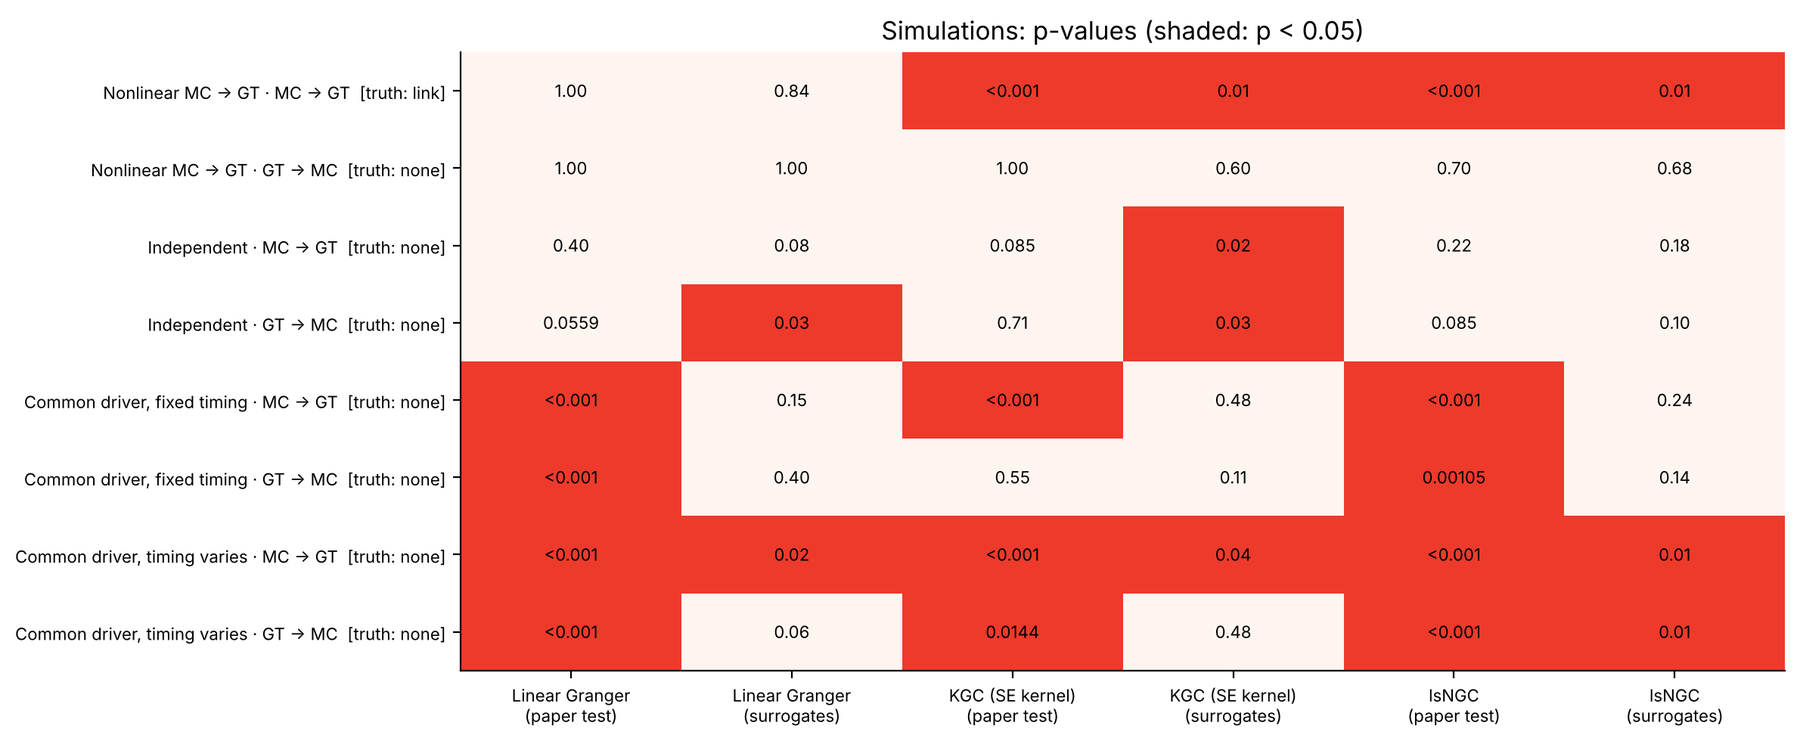
\includegraphics[width=\linewidth]{kg01_simulation_single}
  \caption{p-values of every test for one simulated dataset per scenario (shaded: $p<0.05$). ``Truth'' gives whether a direct link exists.}
  \label{fig:simsingle}
\end{figure}

\begin{figure}[htbp]
  \centering
  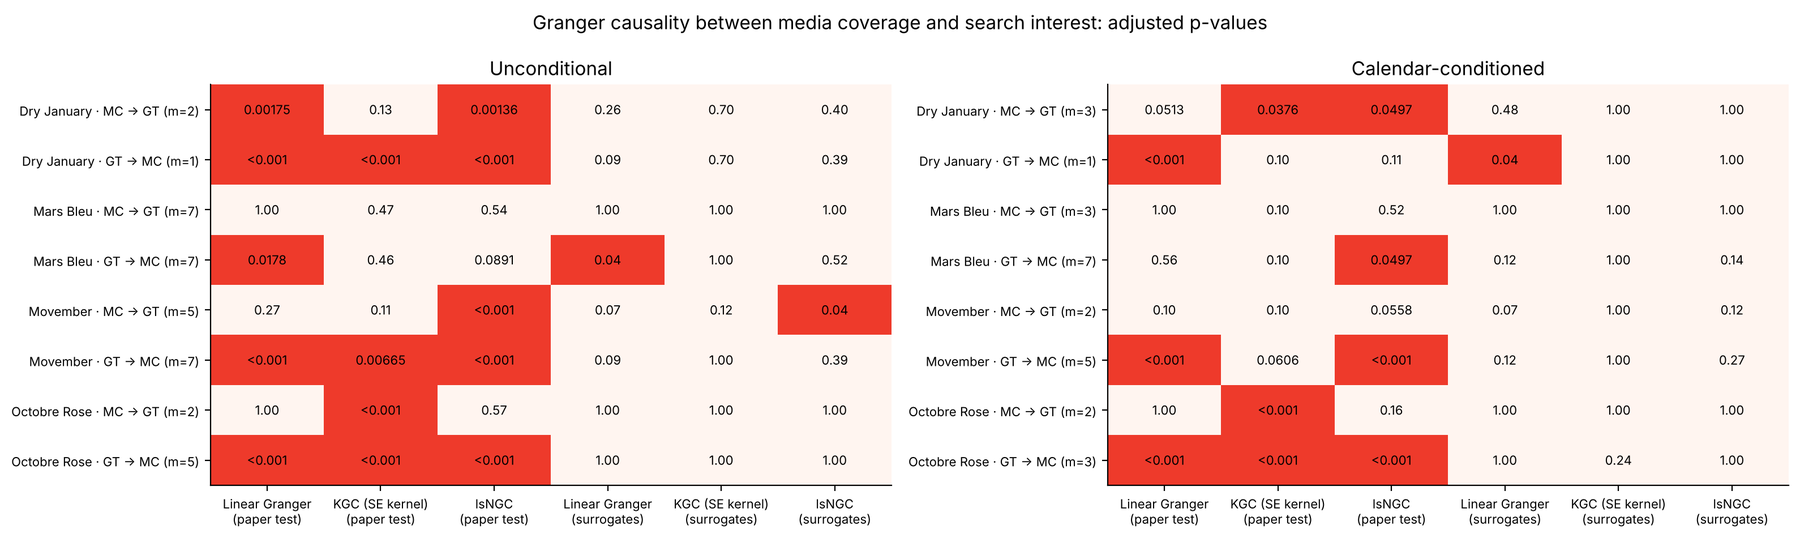
\includegraphics[width=\linewidth]{kg04_main_results}
  \caption{Adjusted p-values of linear Granger causality, KGC (squared-exponential kernel) and lsNGC, with the parametric tests of the original papers and with season-swap surrogates, without (left) and with (right) calendar conditioning. Shaded cells: $p<0.05$. $m$: lag order.}
  \label{fig:main}
\end{figure}

\begin{figure}[htbp]
  \centering
  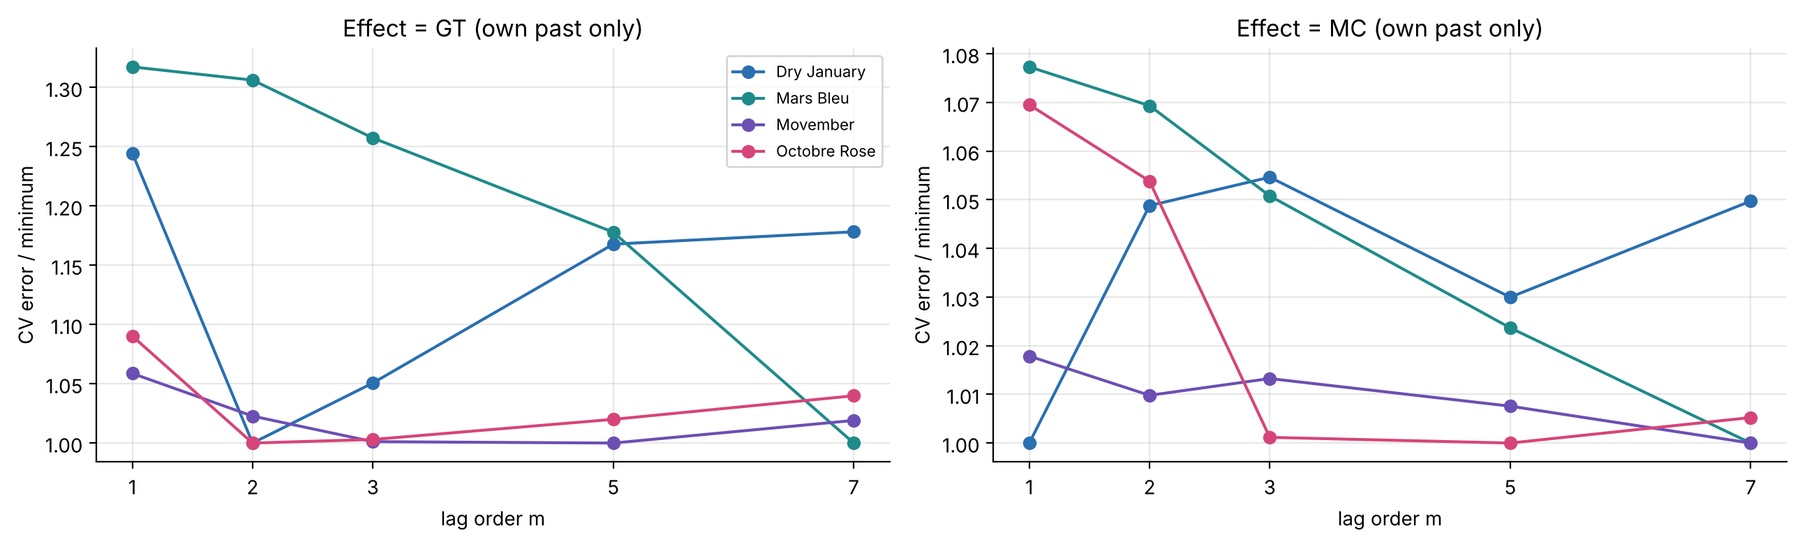
\includegraphics[width=\linewidth]{kg03_lag_selection}
  \caption{Lag-order selection for the nonlinear tests: leave-one-season-out cross-validation error of a kernel ridge model of each effect series on its own past only, relative to its minimum, by lag order $m$.}
  \label{fig:lagsel}
\end{figure}

\begin{figure}[htbp]
  \centering
  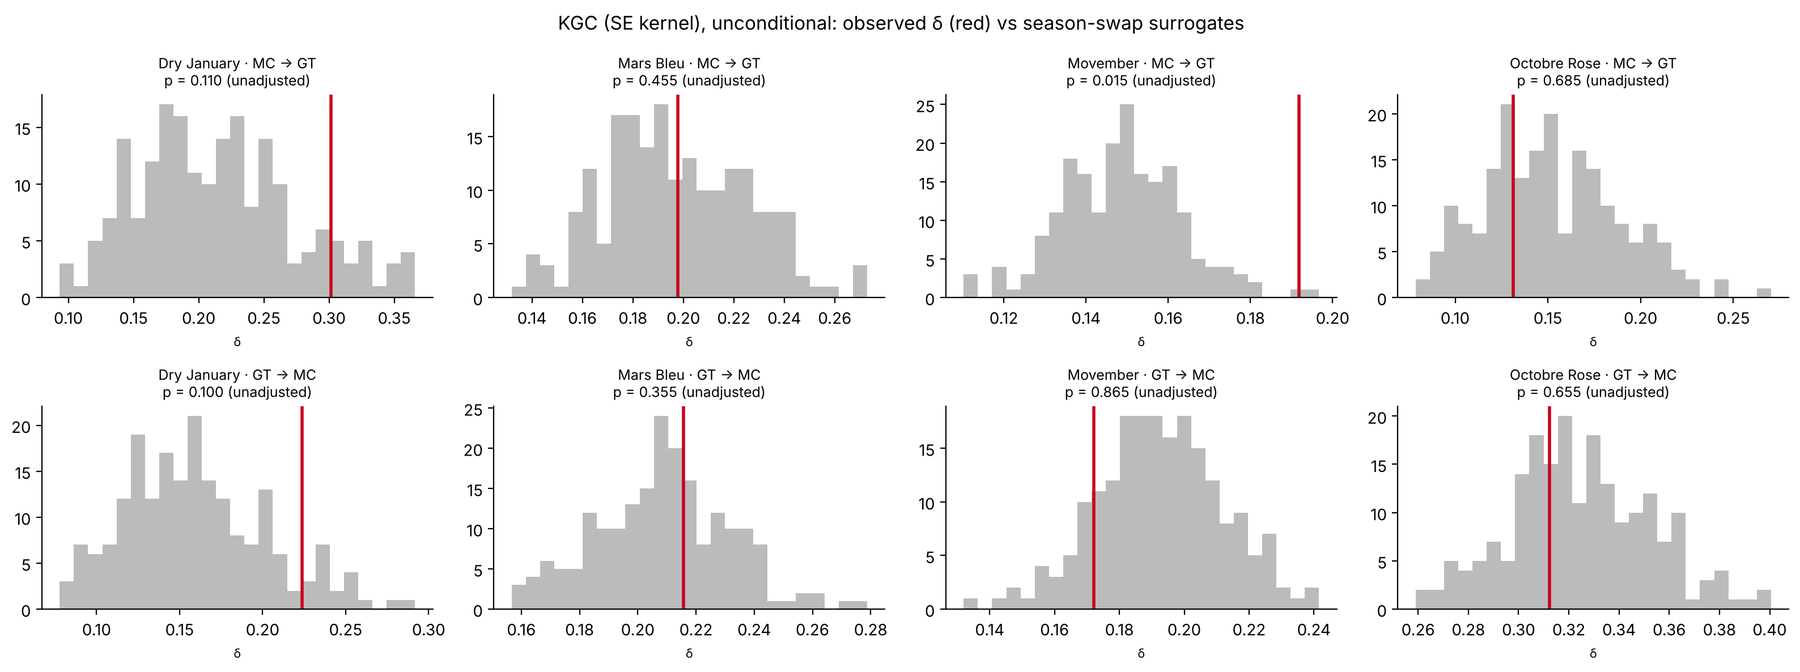
\includegraphics[width=\linewidth]{kg05_null_kgc_se}
  \caption{KGC (squared-exponential kernel), unconditional variant: observed statistic $\delta$ (red line) against its distribution over 199 season-swap surrogates, with unadjusted surrogate p-values.}
  \label{fig:null-kgc}
\end{figure}

\begin{figure}[htbp]
  \centering
  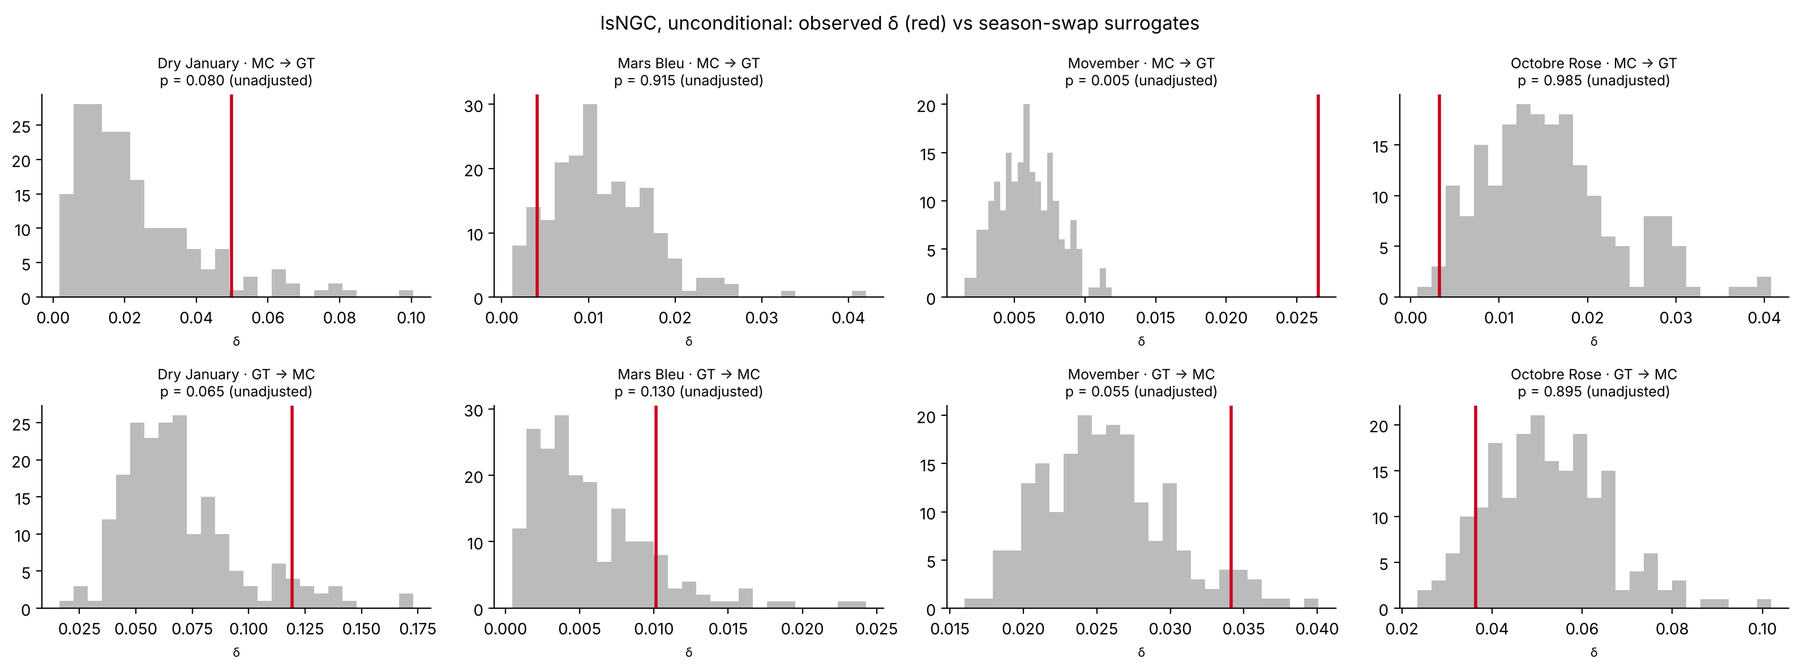
\includegraphics[width=\linewidth]{kg05_null_lsngc}
  \caption{lsNGC, unconditional variant: observed statistic $\delta$ (red line) against its distribution over 199 season-swap surrogates, with unadjusted surrogate p-values.}
  \label{fig:null}
\end{figure}

\begin{figure}[htbp]
  \centering
  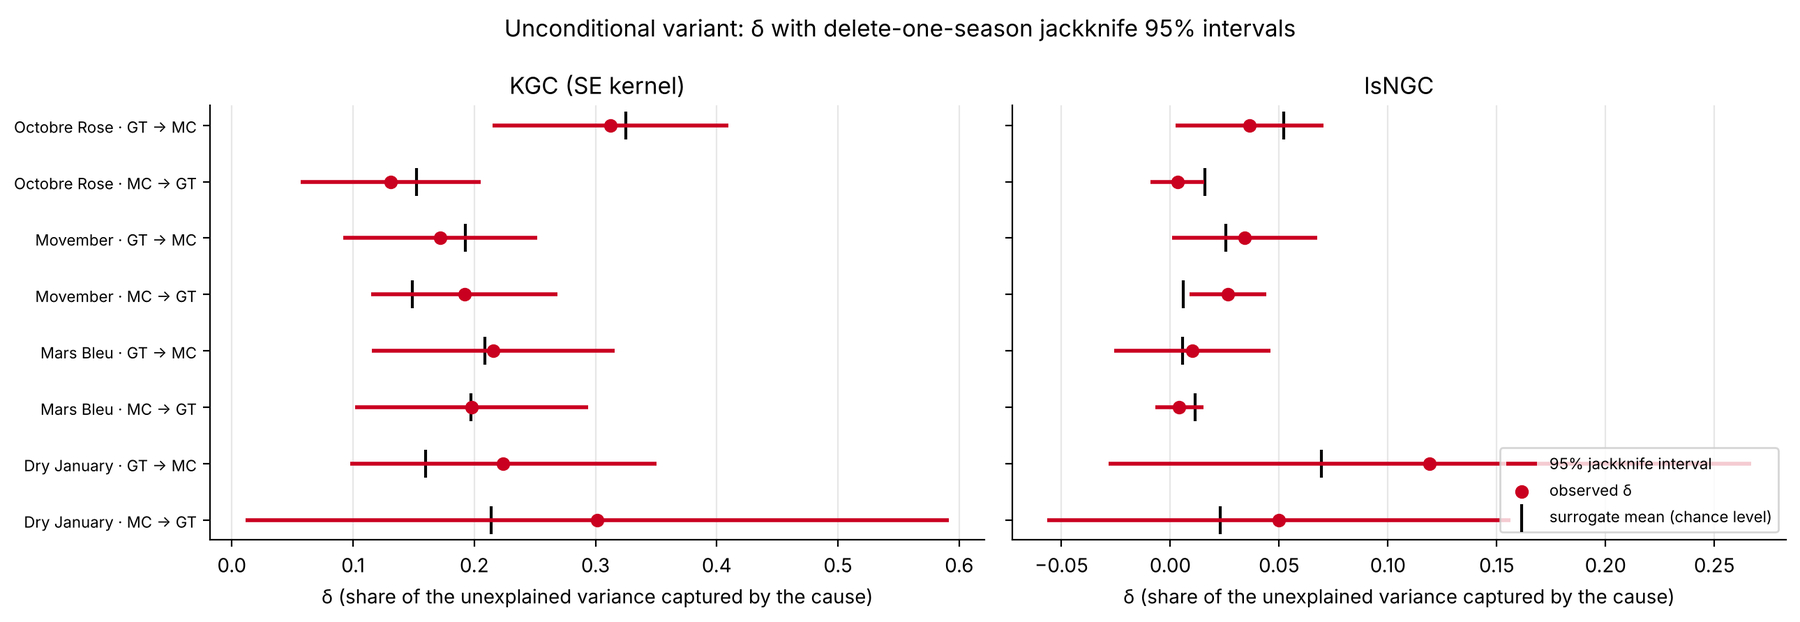
\includegraphics[width=\linewidth]{kg07_jackknife_delta}
  \caption{Unconditional variant: observed statistic $\delta$ (dot) with its 95\% delete-one-season jackknife interval (line) and its chance level (mean over 199 surrogates, vertical tick), for KGC (squared-exponential kernel, left) and lsNGC (right).}
  \label{fig:jkdelta}
\end{figure}

\begin{table}[htbp]
\centering
\caption{lsNGC, unconditional variant, repeated with 10 k-means initialisations (199 surrogates each; Holm correction across the eight tests for each initialisation).}
\label{tab:seeds}
\small
\begin{tabular}{llccc}
\toprule
Campaign & Direction & $\delta$ (min--max) & Surrogate $p$ (min--max) & Significant after Holm \\
\midrule
Dry January  & MC $\to$ GT & 0.038--0.053 & 0.055--0.175 & 0/10 \\
             & GT $\to$ MC & 0.119--0.119 & 0.035--0.090 & 0/10 \\
Mars Bleu    & MC $\to$ GT & 0.003--0.007 & 0.855--0.985 & 0/10 \\
             & GT $\to$ MC & 0.012--0.024 & 0.005--0.060 & 5/10 \\
Movember     & MC $\to$ GT & 0.024--0.028 & 0.005--0.005 & 10/10 \\
             & GT $\to$ MC & 0.031--0.034 & 0.010--0.035 & 0/10 \\
Octobre Rose & MC $\to$ GT & 0.001--0.003 & 0.960--1.000 & 0/10 \\
             & GT $\to$ MC & 0.033--0.039 & 0.865--0.945 & 0/10 \\
\bottomrule
\end{tabular}
\end{table}

\begin{figure}[htbp]
  \centering
  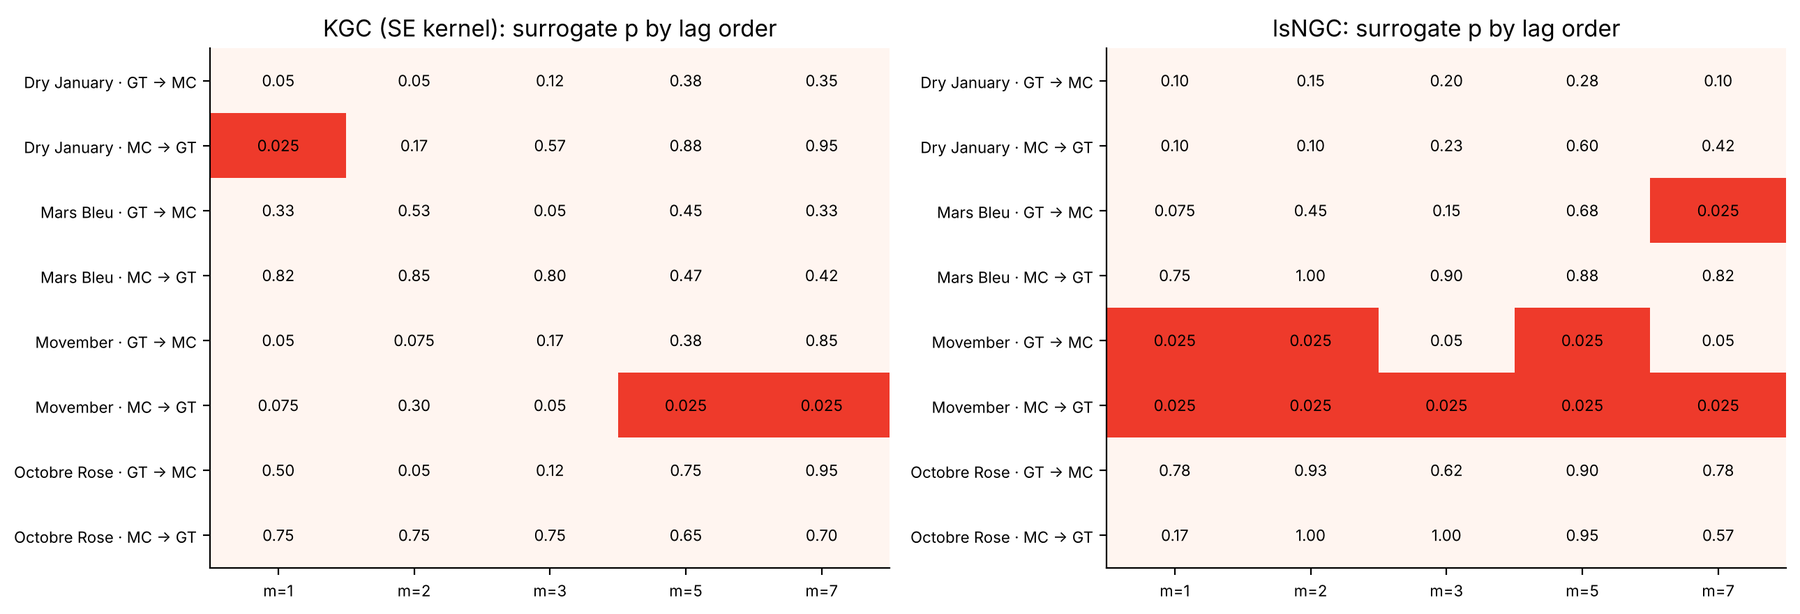
\includegraphics[width=\linewidth]{kg06_lag_sensitivity}
  \caption{Unadjusted surrogate p-values of KGC (squared-exponential kernel, left) and lsNGC (right) by lag order $m$, unconditional variant, with 39 surrogates (smallest attainable value 0.025). Shaded cells: $p<0.05$.}
  \label{fig:lagsens}
\end{figure}

\end{document}
